
%--------------------------------------------------------------
% ĐẠI HỌC BÁCH KHOA HÀ NỘI
% Trường Điện - Điện tử
% Khoa Tự động hóa
%
% MẪU SOẠN THẢO ĐỒ ÁN 1
%--------------------------------------------------------------
\documentclass{thesis}
\usepackage[utf8]{inputenc} % Hỗ trợ mã hóa tiếng Việt
\usepackage[T5]{fontenc} % Mã hóa phông chữ cho tiếng Việt
\usepackage{graphicx} % Để chèn hình ảnh
\usepackage{float} % Kiểm soát vị trí hình và bảng
\usepackage{mathptmx} % Phông Times New Roman
\usepackage{geometry} % Điều chỉnh bố cục trang
\usepackage{xcolor} % Hỗ trợ màu sắc
\usepackage[fontsize=13pt]{scrextend} % Đặt cỡ chữ 13pt
\usepackage{indentfirst} % Thụt đầu dòng đoạn đầu tiên
\usepackage{amsmath} % Hỗ trợ toán học
\usepackage{subcaption} % Hình phụ
\usepackage{booktabs} % Định dạng bảng nâng cao
\usepackage{siunitx} % Hỗ trợ đơn vị SI
\usepackage{multirow} % Bảng nhiều hàng
\usepackage{amsfonts} % Phông chữ toán học
\usepackage{amsmath} % Công thức toán học
\usepackage{textcomp}


% BẮT ĐẦU TÀI LIỆU
\begin{document}

% TẠO TRANG BÌA
\begin{center}
    \vspace{12pt}
    \textbf{\fontsize{15pt}{0pt}\selectfont ĐẠI HỌC BÁCH KHOA HÀ NỘI \\ \vspace{3pt} TRƯỜNG ĐIỆN - ĐIỆN TỬ}
    \vspace{0.5cm}
    
    % CHÈN LOGO (Giả sử logoBK.png tồn tại)
    \begin{figure}[H]
        \centering
        
\includegraphics[width=2cm,height=3cm]{logoBK.png}
    \end{figure}

    % LOẠI ĐỒ ÁN
    \vspace{48pt}
    \fontsize{25pt}{0pt}\selectfont \textbf{ĐỒ ÁN I}
    \vspace{24pt}

    % TIÊU ĐỀ ĐỒ ÁN
    \textbf{\fontsize{17pt}{0pt}\selectfont SO SÁNH ĐỘ CHÍNH XÁC GIỮA MỘT SỐ MÔ HÌNH MẠCH ĐIỆN TƯƠNG ĐƯƠNG CHO PIN LITHIUM-ION }
    \vspace{18pt}

    % TÊN
    \fontsize{14pt}{0pt}\selectfont \textbf{CAO LÂM TÙNG}
    \vspace{3pt}

    % EMAIL
    \fontsize{14pt}{0pt}\selectfont Tung.cl222709@sis.hust.edu.vn
    \vspace{12pt}

    % NGÀNH HỌC
    \fontsize{14pt}{0pt}\selectfont \textbf{Ngành Kỹ thuật Điều khiển và Tự động hóa}
\end{center}
    \vspace{48pt}

    % THÔNG TIN: GIẢNG VIÊN HƯỚNG DẪN, KHOA, TRƯỜNG
    \begin{table}[H]
        \centering
        \begin{tabular}{l l c}
            \textbf{Giảng viên hướng dẫn:} & TS. Nguyễn Duy Đỉnh \vspace{6pt} & \\
            & \vspace{3pt} & \fontsize{10pt}{0pt}\selectfont Chữ ký của GVHD \\
            \textbf{Khoa:} & Tự động hóa \vspace{3pt} \\
            \textbf{Trường:} & Điện - Điện tử
        \end{tabular}
    \end{table}

    % THỜI GIAN
    \begin{center}
        \vspace{48pt}
        \fontsize{14pt}{0pt}\selectfont Hà Nội, 07/2025
    \end{center}

    \thispagestyle{empty}
    \newpage
    \clearpage
    \thispagestyle{empty}
    \cleardoublepage
% THANKS
\section*{LỜI CẢM ƠN}
    \thispagestyle{empty}
Lời đầu tiên, em xin cảm ơn thầy TS. Nguyễn Duy Đỉnh đã tận tình hướng dẫn, hỗ trợ và tạo điều kiện thuận lợi để em có thể hoàn thành đề tài đồ án này.Em cũng xin chân thành cảm ơn anh Ngô Quốc Khánh cùng mọi người trong EVSELab đã luôn sẵn lòng giúp đỡ em trong suốt quá trình thực hiện.Mặc dù đã cố gắng hoàn thiện đồ án một cách tốt nhất, nhưng với thời gian có hạn và vốn kinh nghiệm còn hạn chế, nên nội dung vẫn còn nhiều thiếu sót. Em rất mong nhận được những góp ý quý báu từ thầy cô để hoàn thiện hơn trong những đề tài tiếp theo.


\vspace{6pt}
    \hspace{7cm}Hà Nội, ngày 3 tháng 7 năm 2025
        
        \hspace{8.6cm} Sinh viên thực hiện      % command '\hspace' used to line indents

\vspace{2cm}
    \hspace{9.25cm}\textbf{Cao Lâm Tùng} % change name

\newpage % create a new page
    \thispagestyle{empty} 
        \clearpage
            \thispagestyle{empty}
                \cleardoublepage
    % PHẦN TÓM TẮT
    \section*{TÓM TẮT ĐỒ ÁN}
    \thispagestyle{empty}
    Đồ án tập trung nghiên cứu và so sánh các mô hình mạch điện tương đương (ECM) của pin Lithium-ion (LIB) với tiêu chí về độ phức tạp và chính xác. Đồ án trình bày các cơ sở hình thành của các mô hình ECM. Bên cạnh đó, đồ án cung cấp các phương pháp xác định thông số của từng loại mô hình ECM dựa trên kết quả thí nghiệm HPPC (Hybrid Pulse Power Characterization). Tiếp theo, quá trình sạc CC-CV (Constant Current- Constant Voltage) sẽ được mô phỏng bằng phần mềm PSIM để kiểm tra đáp ứng điện áp của từng mô hình ECM, từ đó so sánh với thực nghiệm và đánh giá dựa vào các loại sai số khác nhau.
    \thispagestyle{empty}
    \cleardoublepage

    % MỤC LỤC
    \tableofcontents
    \thispagestyle{empty}
    \newpage
    \thispagestyle{empty}
    \cleardoublepage
    
% LIST OF SYMBOLS AND ABBREVIATIONS
\pagenumbering{roman}   % Roman numbering: i, ii, iii, iv,...
\section*{DANH MỤC KÝ HIỆU VÀ CHỮ VIẾT TẮT}
\phantomsection \addcontentsline{toc}{section}{\numberline{} DANH MỤC KÝ HIỆU VÀ CHỮ VIẾT TẮT}

% Create table
\begin{tabular}{ l l }
    \hspace{1cm} BEV & \hspace{4cm} Battery Electric Vehicle \\
    \hspace{1cm} BMS & \hspace{4cm} Battery Management System \\
    \hspace{1cm} BTMS & \hspace{4cm} Battery Thermal Management System \\
    \hspace{1cm} CC & \hspace{4cm} Constant Current \\
    \hspace{1cm} CCCV & \hspace{4cm} Constant Current - Constant Voltage \\
    \hspace{1cm} CV & \hspace{4cm} Constant Voltage \\
    \hspace{1cm} ECM & \hspace{4cm} Equivalent Circuit Model \\
    \hspace{1cm} EIS & \hspace{4cm} Electrochemical Impedance Spectroscopy \\
    \hspace{1cm} ESP & \hspace{4cm} Extended Single Particle \\
    \hspace{1cm} EV & \hspace{4cm} Electric Vehicle \\
    \hspace{1cm} FCEV & \hspace{4cm} Fuel Cell Electric Vehicle \\
    \hspace{1cm} HEV & \hspace{4cm} Hybrid Electric Vehicle \\
    \hspace{1cm} HPPC & \hspace{4cm} Hybrid Pulse Power Characterization \\
    \hspace{1cm} LCO & \hspace{4cm} Lithium Cobalt Oxide \\
    \hspace{1cm} LFP & \hspace{4cm} Lithium Iron Phosphate \\
    \hspace{1cm} LIB & \hspace{4cm} Lithium-Ion Battery \\
    \hspace{1cm} LMO & \hspace{4cm} Lithium Manganese Oxide \\
    \hspace{1cm} MSCC & \hspace{4cm} Multistage Constant Current \\
    \hspace{1cm} NCA & \hspace{4cm} Lithium Nickel Cobalt Aluminum Oxide \\
    \hspace{1cm} NCM & \hspace{4cm} Lithium Nickel Cobalt Manganese Oxide \\
    \hspace{1cm} P2D & \hspace{4cm} Pseudo Two-Dimensional \\
    \hspace{1cm} PCM & \hspace{4cm} Phase Change Material \\
    \hspace{1cm} PHEV & \hspace{4cm} Plug-in Hybrid Electric Vehicle \\
    \hspace{1cm} SIB & \hspace{4cm} Sodium-Ion Battery \\
    \hspace{1cm} SOC & \hspace{4cm} State of Charge \\
    \hspace{1cm} SOH & \hspace{4cm} State of Health \\
    \hspace{1cm} SP & \hspace{4cm} Single Particle \\
    \hspace{1cm} SP2D & \hspace{4cm} Simplified Pseudo Two-Dimensional \\
    \hspace{1cm} SSB & \hspace{4cm} Solid-State Battery \\
    \hspace{1cm} VCU & \hspace{4cm} Vehicle Control Unit \\
    \hspace{1cm} VRLA & \hspace{4cm} Valve-Regulated Lead-Acid \\
    \hspace{1cm} ZIB & \hspace{4cm} Zinc-Ion Battery \\
\end{tabular}
\newpage
    \newpage
    % DANH MỤC HÌNH VẼ
    {\let\oldnumberline\numberline
    \renewcommand{\numberline}{Hình~\oldnumberline}
    \listoffigures}
    \phantomsection\addcontentsline{toc}{section}{\numberline{} DANH MỤC HÌNH VẼ}
    \newpage

    % DANH MỤC BẢNG BIỂU
    {\let\oldnumberline\numberline
    \renewcommand{\numberline}{Bảng~\oldnumberline}
    \listoftables}
    \phantomsection\addcontentsline{toc}{section}{\numberline{} DANH MỤC BẢNG BIỂU}
    \newpage

    % CHƯƠNG 1: GIỚI THIỆU CHUNG
    \pagenumbering{arabic}
    \section*{CHƯƠNG 1. GIỚI THIỆU CHUNG}
    \addcontentsline{toc}{section}{\numberline{} CHƯƠNG 1. GIỚI THIỆU CHUNG}
    \setcounter{section}{1}
    \setcounter{subsection}{0}
    \setcounter{figure}{0}
    \setcounter{table}{0}

    \subsection{Tình trạng sử dụng xe điện hiện nay}
    Ngành giao thông vận tải là nguồn phát thải khí nhà kính lớn nhất tại Mỹ, chiếm phần lớn lượng tiêu thụ dầu mỏ và khoảng 30\% tổng nhu cầu năng lượng. Tại Ấn Độ, hơn một nửa số thành phố ô nhiễm nhất thế giới nằm ở đây, với ô nhiễm không khí từ giao thông gây ra các vấn đề sức khỏe nghiêm trọng như bệnh hô hấp và tim mạch. Trong khu vực Trung Đông và Bắc Phi, chất lượng không khí cải thiện đáng kể trong các đợt cách ly COVID-19 tại các thành phố như Cairo, Riyadh và Beirut, cho thấy tiềm năng giảm ô nhiễm từ việc hạn chế xe chạy xăng và diesel. \cite{worldbank}

    Nhận thức được tình trạng cấp bách đó, các cơ quan quản lý ở Châu Âu và Hoa Kỳ đã đặt ra các mục tiêu nhằm giảm lượng khí thải từ ô tô và các phương tiện giao thông hạng nhẹ. Các công nghệ mới cho phương tiện thay thế rất được quan tâm và phát triển, trong đó có xe điện (Electric Vehicle - EV). Hình \ref{fig:doanhso} cho thấy doanh số xe điện toàn cầu tăng trưởng mạnh mẽ từ khoảng 3 triệu (2020) lên gần 18 triệu xe vào năm 2024.Tính đến thời điểm hiện tại, vào giữa năm 2025, xu hướng sử dụng xe điện tiếp tục gia tăng mạnh mẽ, với hơn 20\% tổng doanh số xe mới trên toàn cầu là xe điện, đặc biệt tại các thị trường lớn như Trung Quốc, châu Âu và Hoa Kỳ. Sự gia tăng này được hỗ trợ bởi các chính sách khuyến khích từ chính phủ, sự phát triển của hạ tầng sạc điện và giá thành xe điện ngày càng cạnh tranh, đặc biệt nhờ sự đóng góp lớn từ các nhà sản xuất Trung Quốc. Theo dự báo, số lượng xe điện trên toàn cầu có thể vượt 235 triệu chiếc vào năm 2030, phản ánh cam kết mạnh mẽ trong việc chuyển đổi sang giao thông bền vững \cite{iea2025}.

    \begin{figure}[H]
        \centering
        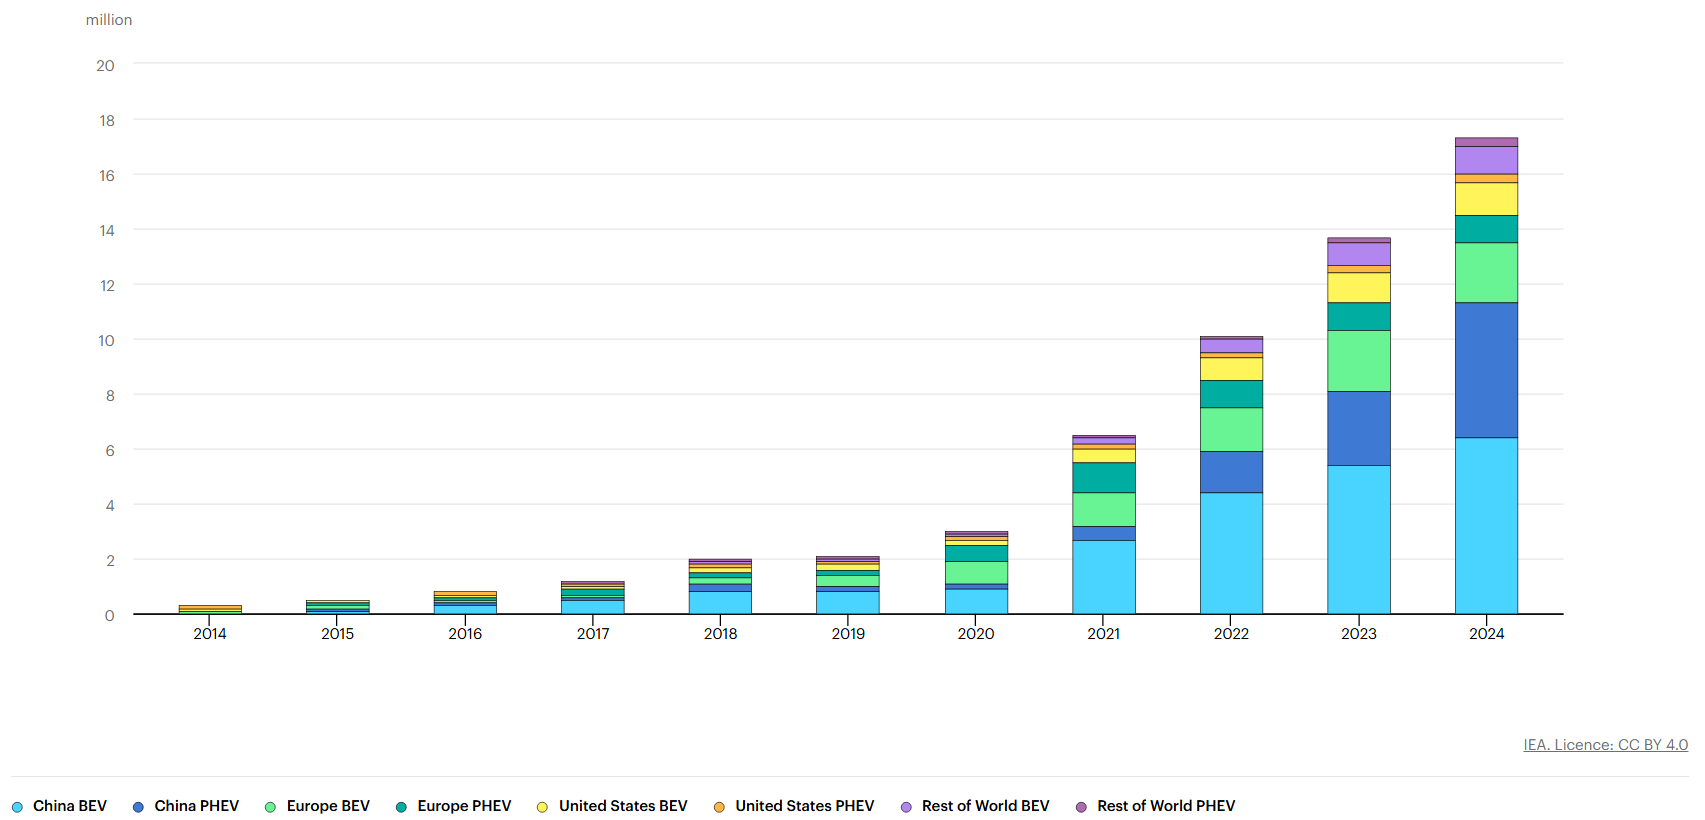
\includegraphics[width=0.8\textwidth]{media/image1.png}
        \caption{Doanh số xe ô tô điện toàn cầu từ năm 2014 đến năm 2024}
        \label{fig:doanhso}
    \end{figure}

    Xe điện được chia thành 4 loại chính dựa trên nguồn năng lượng, bao gồm xe điện lai xăng có thể cắm sạc (Plug-in Hybrid Electric Vehicle - PHEV), xe điện lai xăng không cắm sạc (Hybrid Electric Vehicle - HEV), xe điện dùng pin (Battery Electric Vehicle - BEV) và xe điện dùng pin nhiên liệu (Fuel Cell Electric Vehicle - FCEV). Trong số đó, BEV được coi là lựa chọn tiên tiến và thân thiện với môi trường nhất, do chỉ thuần túy sử dụng năng lượng lấy từ pin mà không kết hợp với động cơ đốt trong như PHEV \cite{yilmaz2012}. Việc quan tâm đến các loại xe điện khác nhau trở nên cần thiết do sự khác biệt trong công nghệ và ứng dụng thực tiễn của chúng, từ việc đáp ứng nhu cầu đa dạng của người dùng đến việc giải quyết các thách thức về cơ sở hạ tầng và nguồn năng lượng. Điều này giúp tối ưu hóa việc áp dụng xe điện trong các bối cảnh khác nhau, từ đô thị đông đúc đến vận tải đường dài.

    \subsection{Tổng quan về pin Lithium-Ion}
    Sự gia tăng mạnh mẽ của xe điện đòi hỏi sự quan tâm đặc biệt đến pin xe điện bởi chúng là yếu tố cốt lõi quyết định hiệu suất, tuổi thọ và chi phí vận hành. Pin không chỉ ảnh hưởng trực tiếp đến quãng đường di chuyển, thời gian sạc và độ an toàn của xe, mà còn là thách thức lớn trong việc quản lý nhiệt độ và tái chế để giảm tác động môi trường. Với nhu cầu nguyên liệu thô như lithium và cobalt ngày càng tăng, cùng áp lực lên lưới điện và cơ sở hạ tầng sạc, việc nghiên cứu và tối ưu hóa pin trở nên cấp thiết để đảm bảo sự phát triển bền vững của ngành giao thông. 
    
    Trong số các loại công nghệ pin được sử dụng cho xe, pin Lithium-Ion (LIB) là ứng cử viên sáng giá bậc nhất, trở thành công nghệ cốt lõi của xe điện. So với các loại pin khác như Valve-Regulated Lead-Acid (VRLA), Sodium-Ion (SIB), Zinc-Ion (ZIB), hoặc các công nghệ pin thay thế, LIB có những ưu điểm nổi bật như mật độ năng lượng cao, hiệu suất sạc/xả cao, tuổi thọ chu kỳ dài, khả năng sạc nhanh, trọng lượng nhẹ, thân thiện với môi trường \cite{chen2012}.

    Pin Lithium-Ion bao gồm các thành phần chính sau (Hình \ref{fig:cautao}):
    \begin{itemize}
        \item \textbf{Điện cực dương (Cathode):} Thường sử dụng các vật liệu như Lithium Cobalt Oxide (LCO), Lithium Iron Phosphate (LFP), Lithium Manganese Oxide (LMO), Lithium Nickel Cobalt Manganese Oxide (NCM), hoặc Lithium Nickel Cobalt Aluminum Oxide (NCA). Cathode quyết định phần lớn mật độ năng lượng và độ ổn định của pin.
        \item \textbf{Điện cực âm (Anode):} Thông thường là graphite hoặc Lithium Titanium Oxide (LTO). Anode ảnh hưởng đến khả năng sạc nhanh và tuổi thọ pin.
        \item \textbf{Chất điện giải (Electrolyte):} Là dung dịch hoặc chất rắn dẫn ion Lithium giữa cathode và anode, thường là muối Lithium (như LiPF$_6$) trong dung môi hữu cơ. Trong các pin trạng thái rắn (Solid-State Battery - SSB), chất điện giải rắn được sử dụng để tăng độ an toàn.
        \item \textbf{Màng ngăn (Separator):} Một lớp polymer mỏng ngăn cách cathode và anode, cho phép ion Lithium đi qua nhưng ngăn chặn sự tiếp xúc trực tiếp để tránh ngắn mạch.
        \item \textbf{Vỏ pin (Casing):} Thường làm bằng kim loại hoặc vật liệu composite để bảo vệ các thành phần bên trong và đảm bảo an toàn nhiệt/điện.
    \end{itemize}

    \begin{figure}[H]
        \centering
        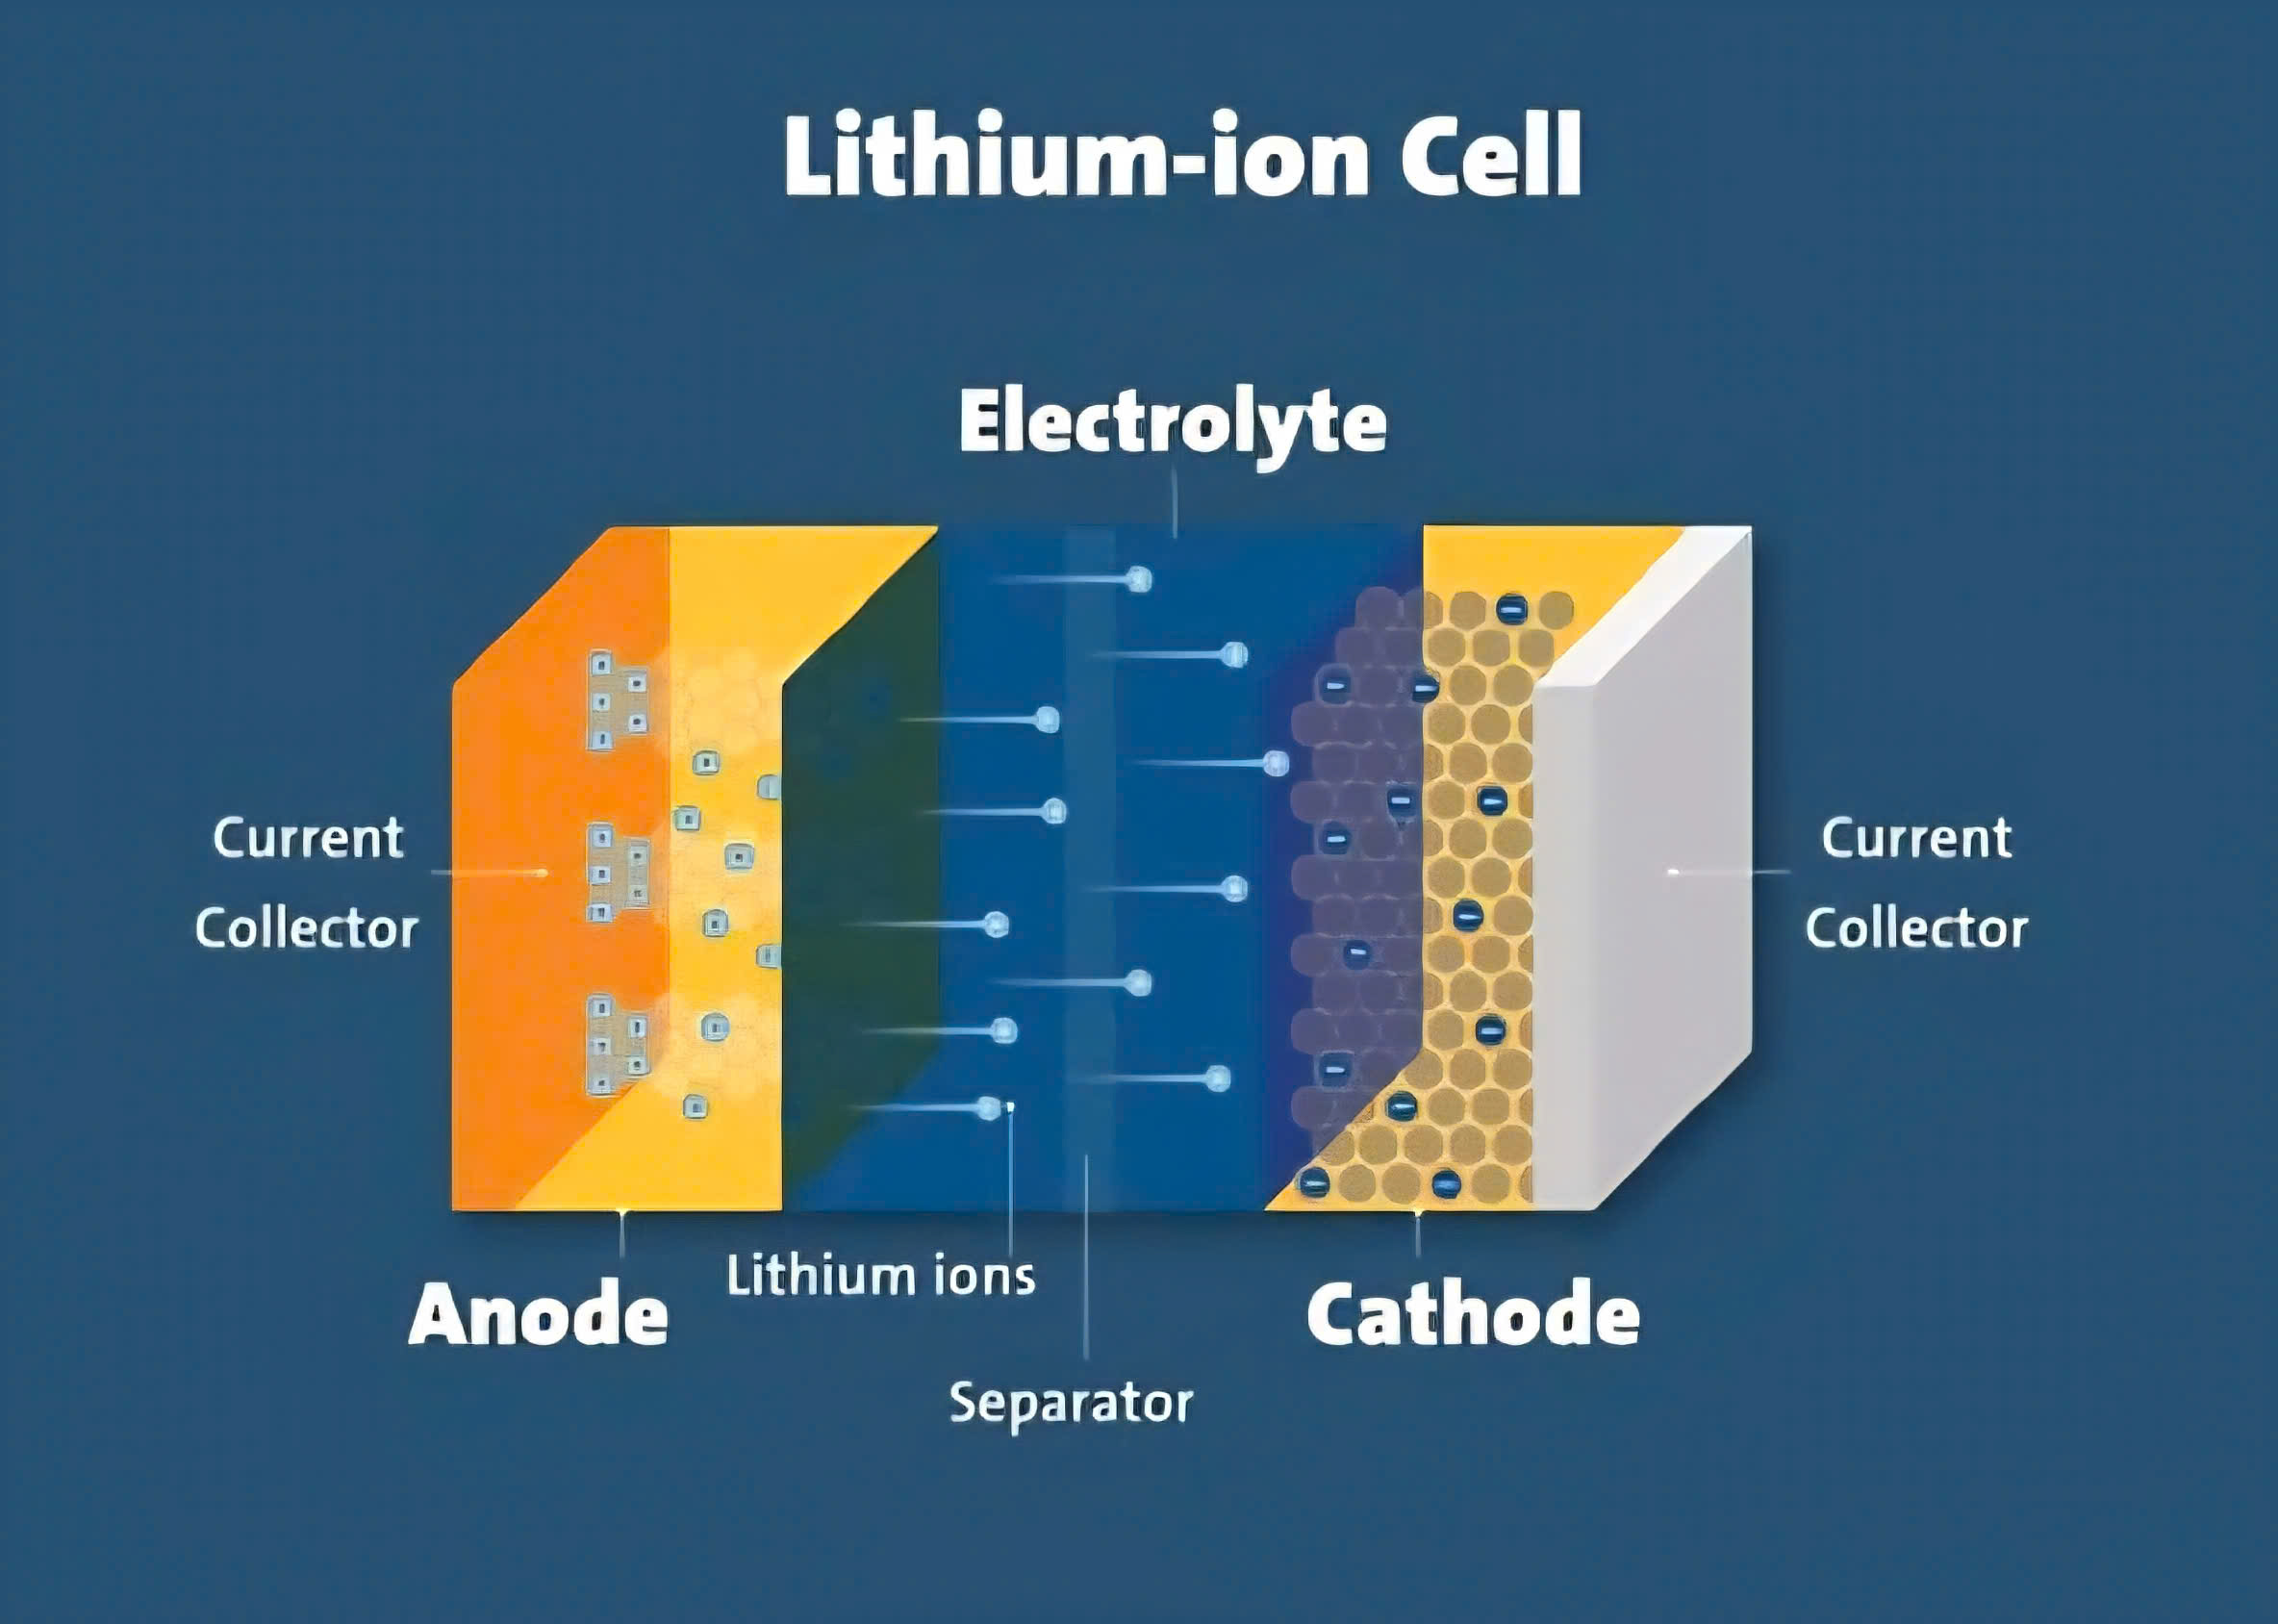
\includegraphics[width=0.8\textwidth]{media/image2.jpg}
        \caption{Cấu tạo pin Lithium-Ion}
        \label{fig:cautao}
    \end{figure}

    Pin Lithium-Ion được phân loại dựa trên vật liệu cathode hoặc cấu trúc hóa học, bao gồm \cite{weiliu2022}:

    \begin{itemize}
        \item \textbf{Lithium Cobalt Oxide (LCO):} Loại pin này sở hữu mật độ năng lượng cao, thường được ứng dụng trong các thiết bị điện tử tiêu dùng như điện thoại thông minh và máy tính xách tay nhờ khả năng lưu trữ năng lượng vượt trội. Tuy nhiên, trong lĩnh vực xe điện (EV), LCO ít phổ biến do chi phí sản xuất cao và độ ổn định hóa học thấp, làm tăng nguy cơ quá nhiệt và giảm hiệu quả khi sử dụng trong điều kiện khắc nghiệt.
        \item \textbf{Lithium Iron Phosphate (LFP):} Pin LFP nổi bật với tính an toàn cao nhờ khả năng chịu nhiệt tốt và tuổi thọ chu kỳ dài, cùng với chi phí sản xuất thấp. Tuy nhiên, mật độ năng lượng của nó thấp hơn so với các loại pin khác, dẫn đến phạm vi hoạt động hạn chế. Do đó, LFP thường được sử dụng trong các dòng xe điện giá rẻ hoặc xe buýt điện, nơi ưu tiên sự an toàn và chi phí hơn là hiệu suất năng lượng cao.
        \item \textbf{Lithium Manganese Oxide (LMO):} Loại pin này có ưu điểm về độ ổn định nhiệt tốt và chi phí sản xuất thấp, phù hợp với các ứng dụng cần an toàn trong môi trường vận hành đa dạng. Tuy nhiên, LMO lại có mật độ năng lượng và tuổi thọ chu kỳ thấp hơn so với các loại pin như Lithium Nickel Cobalt Manganese Oxide (NCM) hoặc Lithium Nickel Cobalt Aluminum Oxide (NCA), khiến nó ít được ưu tiên trong các mẫu xe điện hiện đại.
        \item \textbf{Lithium Nickel Cobalt Manganese Oxide (NCM):} NCM được xem là một lựa chọn cân bằng giữa mật độ năng lượng, tuổi thọ chu kỳ và mức độ an toàn. Với sự tối ưu hóa này, NCM hiện là loại pin phổ biến nhất được sử dụng trong các mẫu xe điện trên thị trường, nhờ khả năng cung cấp hiệu suất cao và độ bền ổn định, đáp ứng tốt nhu cầu đa dạng của người dùng.
        \item \textbf{Lithium Nickel Cobalt Aluminum Oxide (NCA):} Pin NCA nổi bật với mật độ năng lượng rất cao, lý tưởng cho các dòng xe điện hiệu suất cao, chẳng hạn như các mẫu xe của Tesla. Tuy nhiên, loại pin này đòi hỏi quản lý nhiệt nghiêm ngặt do nguy cơ quá nhiệt cao, đòi hỏi hệ thống quản lý pin (BMS) tiên tiến để đảm bảo an toàn và hiệu quả trong vận hành.
    \end{itemize}
    \begin{figure}[H]
        \centering
        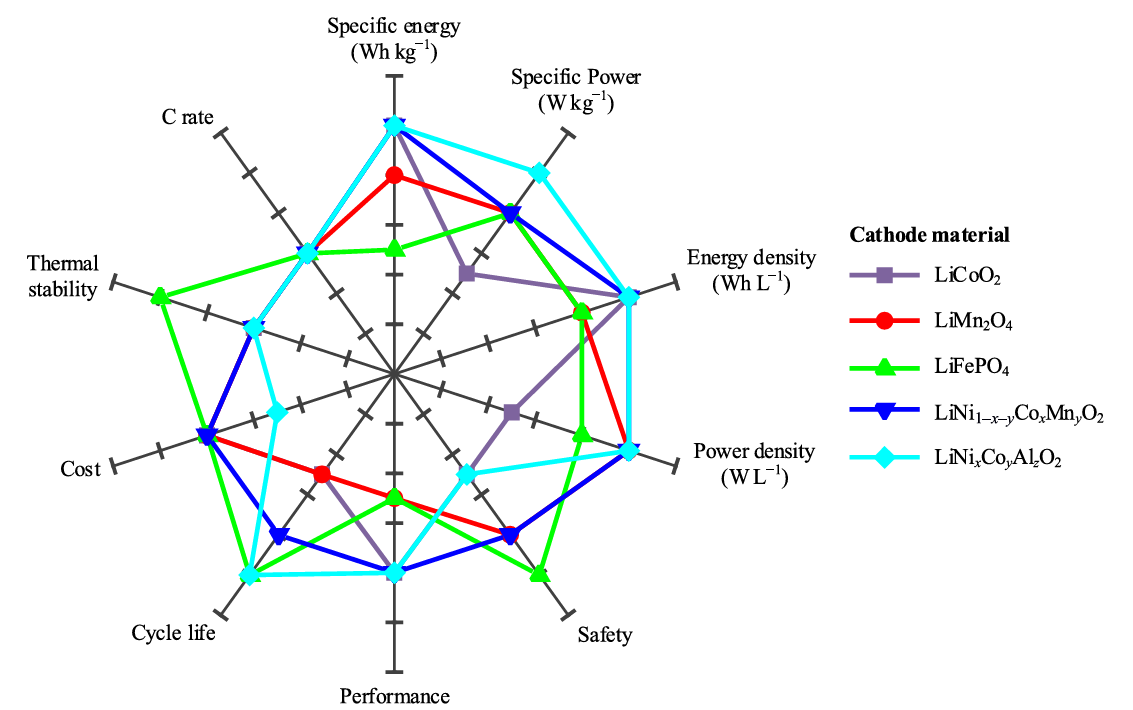
\includegraphics[width=0.8\textwidth]{media/image3.png}
        \caption{Biểu đồ so sánh các loại pin Lithium-Ion}
        \label{fig:so_sanh_pin}
    \end{figure}

Sự so sánh các loại pin Lithium-ion như LCO, LFP, LMO, NCM, và NCA (Hình 1.3.) cho thấy mỗi loại có ưu nhược điểm riêng về mật độ năng lượng, tuổi thọ, an toàn và chi phí. NCM và NCA phù hợp cho xe điện hiệu suất cao nhờ mật độ năng lượng cao, trong khi LFP ưu tiên an toàn và chi phí thấp cho xe giá rẻ. LCO và LMO ít phổ biến trong xe điện do hạn chế về độ ổn định và hiệu suất. Những khác biệt này định hướng lựa chọn công nghệ pin theo nhu cầu cụ thể, thúc đẩy phát triển hệ thống quản lý pin để tối ưu hóa hiệu quả và an toàn.

    Pin Lithium-Ion hoạt động dựa trên quá trình di chuyển của các ion Lithium giữa hai điện cực thông qua chất điện giải (Hình \ref{fig:nguyenly}) \cite{weiliu2022}:

    \begin{itemize}
        \item \textbf{Khi sạc:} Các ion Lithium di chuyển từ cathode (điện cực dương) qua chất điện giải đến anode (điện cực âm). Đồng thời, electron di chuyển qua mạch ngoài từ cathode đến anode, tạo ra dòng điện. Tại anode, ion Lithium được lưu trữ trong cấu trúc vật liệu, thường là graphite, nhờ khả năng hấp thụ và giữ ion hiệu quả.
        \item \textbf{Khi xả (phóng điện):} Các ion Lithium di chuyển ngược từ anode về cathode qua chất điện giải. Electron di chuyển qua mạch ngoài từ anode đến cathode, cung cấp năng lượng cho xe điện, bao gồm động cơ và các hệ thống phụ trợ.
    \end{itemize}

    \begin{figure}[H]
        \centering
        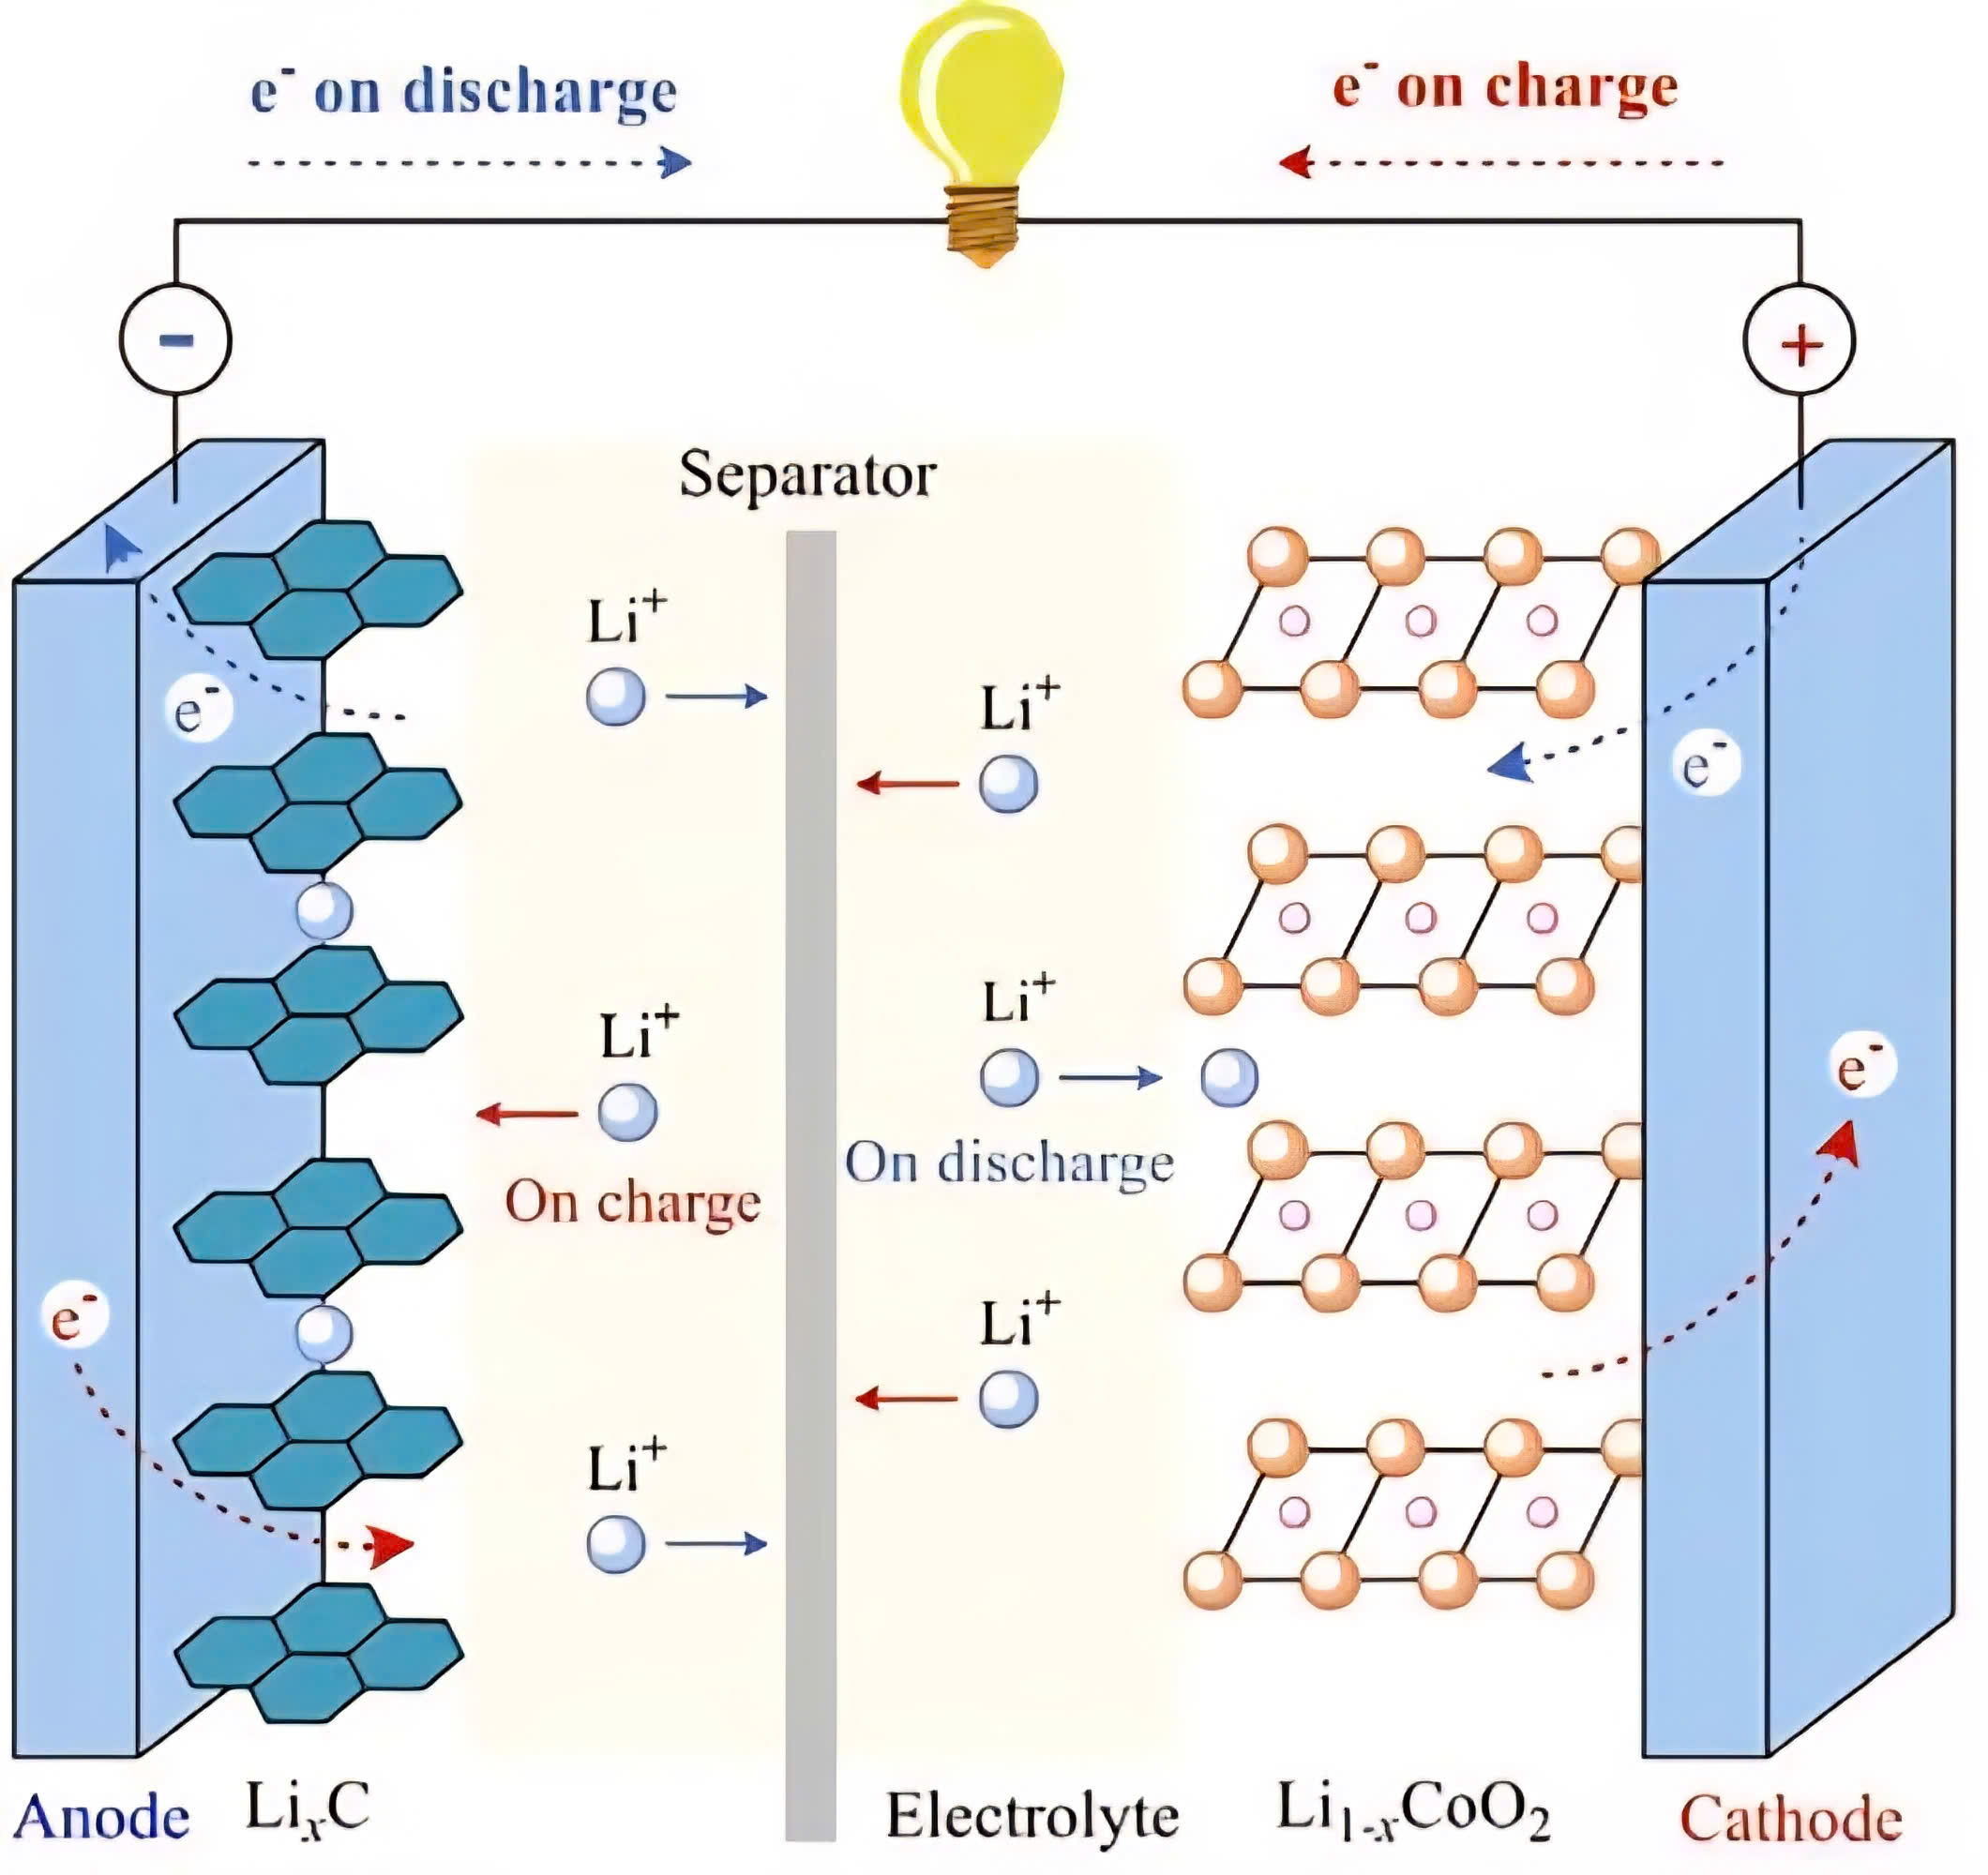
\includegraphics[width=0.8\textwidth]{media/image4.jpg}
        \caption{Nguyên lý hoạt động của pin Lithium-Ion}
        \label{fig:nguyenly}
    \end{figure}

    \subsection{Hệ thống quản lý pin (BMS)}
    Hệ thống quản lý pin (BMS) là một thành phần cốt lõi trong xe điện (EV) và xe lai (HEV), đảm bảo an toàn, hiệu suất và tuổi thọ của pin. BMS hoạt động như “bộ não” của gói pin, giúp khai thác tối đa ưu thế của pin LIB trong khi giảm thiểu các rủi ro như cháy nổ hoặc suy giảm nhanh chóng. Pin trong EV thường bao gồm hàng trăm tế bào pin nối tiếp hoặc song song để đáp ứng yêu cầu công suất và điện áp cao, do đó cần một BMS được thiết kế cẩn thận để quản lý hệ thống phức tạp này .

    BMS thực hiện nhiều chức năng quan trọng để quản lý pin Lithium-Ion trong xe điện \cite{weiliu2022} (Hình \ref{fig:bms}), bao gồm:

    \begin{itemize}
        \item \textbf{Giám sát trạng thái pin:}
        \begin{itemize}
            \item \textbf{Trạng thái sạc (SOC - State of Charge):} Xác định mức năng lượng còn lại trong pin (tính bằng phần trăm), giúp người dùng biết phạm vi hoạt động còn lại.
            \item \textbf{Trạng thái sức khỏe (SOH - State of Health):} Đánh giá mức độ suy giảm của pin qua thời gian, dự đoán tuổi thọ còn lại.
            \item \textbf{Đo lường các thông số:} Theo dõi điện áp, dòng điện, và nhiệt độ của từng tế bào pin trong gói pin.
        \end{itemize}
        \item \textbf{Cân bằng pin (Cell Balancing):} Trong gói pin, các cell pin có thể có mức sạc không đồng đều do sự khác biệt nhỏ trong sản xuất hoặc sử dụng. BMS điều chỉnh để đảm bảo tất cả các tế bào được sạc/xả đồng đều, tránh tình trạng một số tế bào bị quá tải hoặc quá xả. Phương pháp cân bằng bao gồm thụ động (xả năng lượng dư thừa qua điện trở) và chủ động (chuyển năng lượng giữa các tế bào).
        \item \textbf{Quản lý nhiệt (Thermal Management):} BMS phối hợp với hệ thống quản lý nhiệt (BTMS) để giữ nhiệt độ pin trong khoảng an toàn (thường từ 20°C đến 40°C). Các biện pháp làm mát bao gồm làm mát bằng không khí, chất lỏng, hoặc vật liệu chuyển pha (PCM).
        \item \textbf{Bảo vệ an toàn:} Ngăn chặn quá tải (overcharge) và quá xả (over-discharge) bằng cách ngắt mạch khi cần. Phát hiện ngắn mạch hoặc rò rỉ điện, bảo vệ cả pin và người dùng. Giám sát các lỗi tiềm ẩn (như hỏng tế bào, kết nối lỏng lẻo) và đưa ra cảnh báo.
        \item \textbf{Giao tiếp và điều khiển:} BMS giao tiếp với hệ thống điều khiển xe (Vehicle Control Unit - VCU) để cung cấp dữ liệu về trạng thái pin, từ đó điều chỉnh công suất động cơ hoặc chế độ lái. Cung cấp thông tin cho người dùng qua bảng điều khiển, chẳng hạn như phạm vi hoạt động còn lại hoặc thời gian sạc.
    \end{itemize}

    \begin{figure}[H]
        \centering
        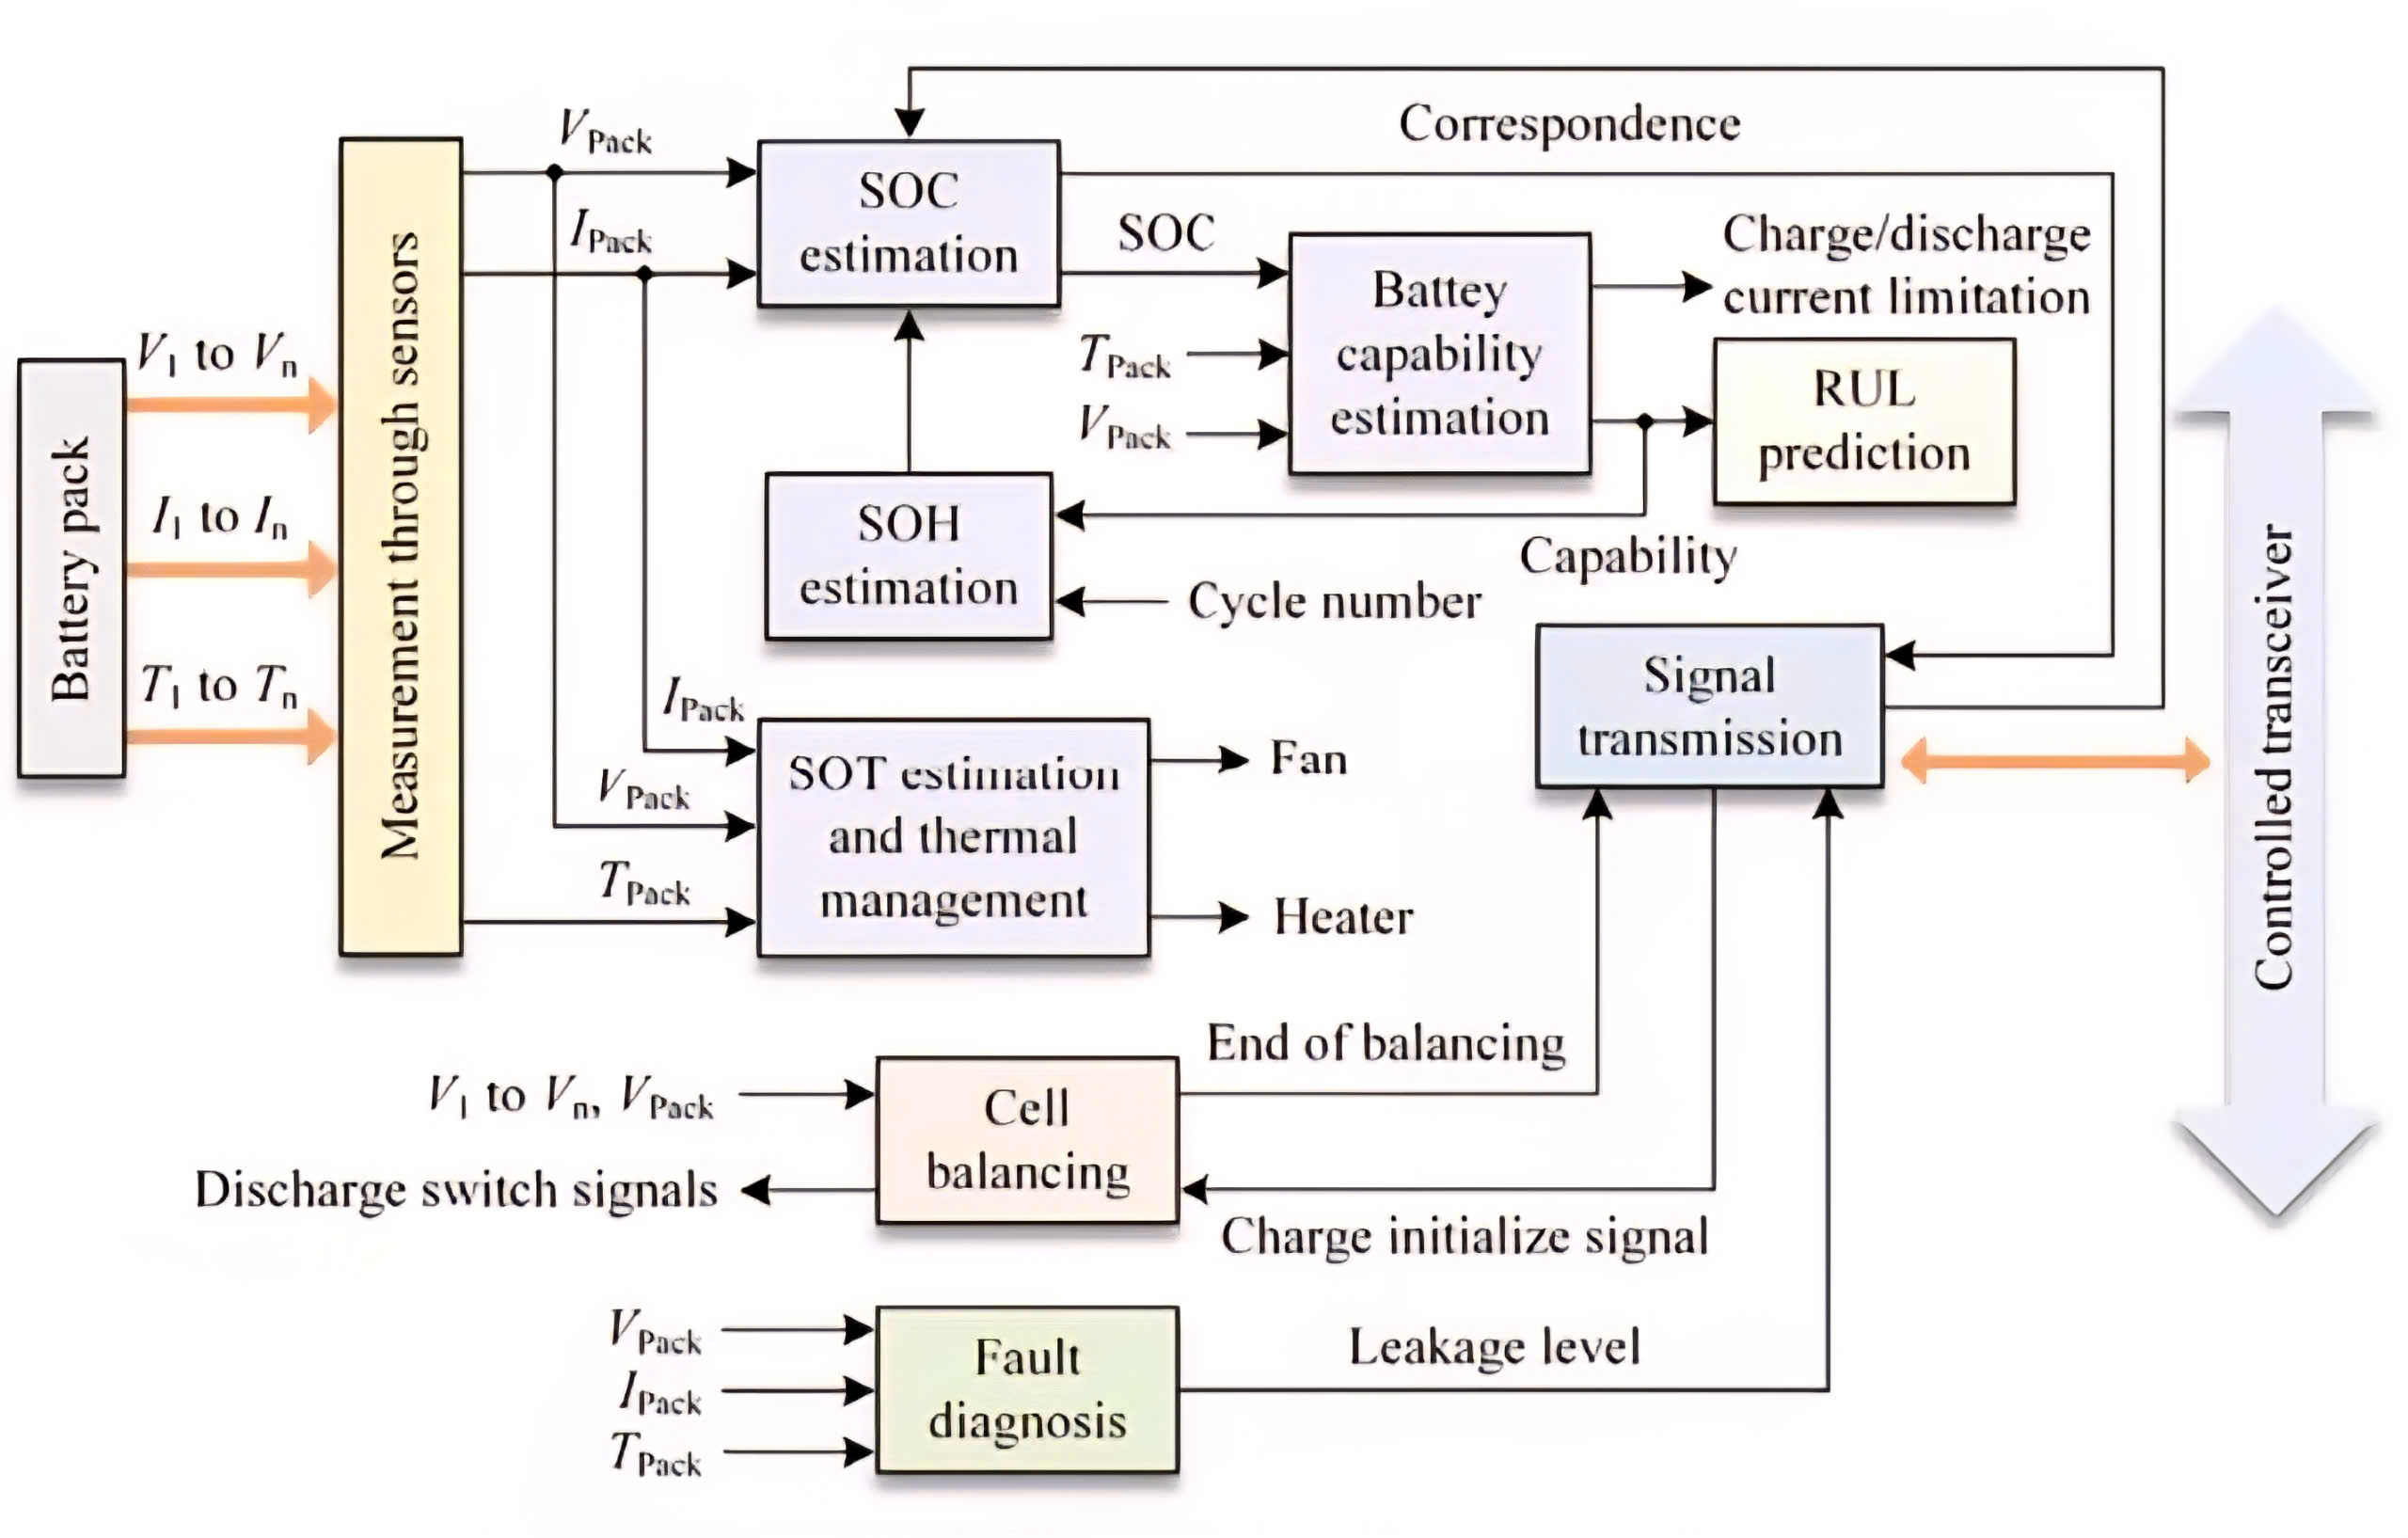
\includegraphics[width=0.8\textwidth]{media/image5.jpg}
        \caption{Sơ đồ khối của BMS cho xe điện}
        \label{fig:bms}
    \end{figure}

    Trong đó, mô hình hóa pin là bước khởi đầu quan trọng trong thiết kế BMS, giúp phân tích hành vi pin, giám sát trạng thái, điều khiển thời gian thực, quản lý nhiệt và chẩn đoán \cite{shen2022}. Tuy nhiên, quá trình phức tạp bên trong pin đòi hỏi mô hình phải mô phỏng chính xác các yếu tố như phân cực, lão hóa và suy giảm hiệu suất. Sự đa dạng về loại pin và cấu trúc càng làm tăng thách thức này. Do đó, các nhà nghiên cứu đã phát triển đa dạng mô hình pin, bao gồm mô hình nhiệt, mô hình điện hóa, mô hình mạch tương đương,… nhằm mô phỏng toàn diện hoạt động của pin.
    
    Một cách tiếp cận phổ biến là sử dụng mô hình điện tương đương , trong đó pin được biểu diễn bằng các thành phần điện như điện trở, tụ điện và nguồn điện áp. Phương pháp này đơn giản và dễ tích hợp vào hệ thống quản lý pin , cho phép dự đoán trạng thái sạc (SOC) và trạng thái sức khỏe (SOH) một cách nhanh chóng.Mỗi mô hình có ưu điểm và hạn chế riêng, tùy thuộc vào mục đích sử dụng. Chẳng hạn, mô hình đơn giản có thể dễ triển khai nhưng thiếu chính xác khi mô phỏng các trạng thái động của pin, trong khi mô hình phức tạp hơn có thể cung cấp kết quả chi tiết hơn nhưng đòi hỏi tính toán phức tạp. Việc so sánh độ chính xác giữa các mô hình giúp xác định mô hình nào phù hợp nhất với ứng dụng cụ thể. So sánh độ chính xác giữa các mô hình mạch điện tương đương là cần thiết để đảm bảo rằng mô hình được chọn có thể phản ánh chính xác hành vi thực tế của pin trong các điều kiện hoạt động khác nhau, từ đó cung cấp dữ liệu đáng tin cậy cho việc thiết kế và tối ưu hóa hệ thống sử dụng pin.
    
    \subsection{Phạm vi đồ án}
    Cấu trúc Đồ án được trình bày theo các phần như sau: Chương 2 là cơ sở và phân loại các mô hình pin. Tại Chương 3, phương pháp được sử dụng để xác định thông số của từng loại mô hình được làm rõ. Sau đó, Chương 4 trình bày kết quả xác định các thông số mô hình pin từ thực nghiệm. Cuối cùng, chương 5 thực hiện việc đánh giá, so sánh sai số giữa các mô hình pin và thực nghiệm, cuối cùng là đưa ra kết luận. Do không có tiêu chuẩn cụ thể nào về sai số được phép cho các mô hình, nên đồ án này sử dụng tài liệu \cite{he2011} để lựa chọn mô hình với RMSE < 0.5V, MPE < 3\% và phương sai < 0.08\(V^2\)
    \newpage
% CHƯƠNG 2
    \section*{CHƯƠNG 2. CƠ SỞ MÔ HÌNH HÓA PIN LITHIUM-ION}
    \addcontentsline{toc}{section}{\numberline{} CHƯƠNG 2. CƠ SỞ MÔ HÌNH HÓA PIN LITHIUM-ION}
    \setcounter{section}{2}
    \setcounter{subsection}{0}
    \setcounter{figure}{0}
    \setcounter{table}{0}
    \subsection{Mô hình nhiệt}
    Mô hình nhiệt trong hệ thống quản lý pin (BMS) được sử dụng để mô phỏng sự tạo nhiệt và truyền nhiệt trong pin, đảm bảo quản lý nhiệt độ hiệu quả nhằm bảo vệ an toàn và tối ưu hóa hiệu suất. Nhiệt độ bên trong pin có thể chênh lệch đáng kể so với bề mặt, lên đến 12°C trong các ứng dụng công suất cao, do đó mô hình hóa nhiệt đóng vai trò quan trọng trong việc ngăn ngừa quá nhiệt và kéo dài tuổi thọ pin. Các mô hình nhiệt bao gồm mô hình tạo nhiệt, mô hình truyền nhiệt, mô hình nhiệt hai giai đoạn, và mô hình nhiệt giảm bậc, mỗi loại được thiết kế để giải quyết các khía cạnh khác nhau của quá trình nhiệt trong pin \cite{kailong2019}.

    Mô hình tạo nhiệt tập trung vào việc tính toán các nguồn nhiệt sinh ra trong pin, bao gồm tổn thất ohmic do điện trở nội, tổn thất do chênh lệch điện thế giữa điện áp vận hành và điện áp mạch hở, cũng như nhiệt do thay đổi entropy và hiệu ứng Joule. Những yếu tố này được kết hợp để cung cấp một bức tranh toàn diện về lượng nhiệt được tạo ra, giúp BMS xác định các điều kiện nguy hiểm. Trong khi đó, mô hình truyền nhiệt mô phỏng cách nhiệt được phân bố trong không gian ba chiều hoặc một chiều, cho phép phát hiện các điểm nóng và điều chỉnh chiến lược làm mát hoặc làm nóng phù hợp \cite{kailong2019}.

    Mô hình nhiệt hai giai đoạn giả định nhiệt độ được phân bố đều trong pin, chia thành nhiệt độ bên trong và nhiệt độ bề mặt, cung cấp một phương pháp đơn giản nhưng hiệu quả để ước lượng nhiệt độ thời gian thực. Đặc biệt, mô hình này được ứng dụng trong các tình huống sạc nhanh, nơi kiểm soát nhiệt độ là yếu tố then chốt. Ngoài ra, mô hình nhiệt giảm bậc được phát triển để giảm chi phí tính toán của các mô hình phức tạp hơn, sử dụng các kỹ thuật như phân rã giá trị đơn, giúp phù hợp hơn với các hệ thống BMS trong thực tế \cite{kailong2019}.

    \subsection{Mô hình điện hóa}
    Mô hình điện hóa là dạng mô hình xuất phát trực tiếp từ bản chất điện hóa của pin, sử dụng các nguyên lý và phương trình điện hóa để giải thích chi tiết hoạt động bên trong của pin. Mô hình này đã được nhiều nhà nghiên cứu áp dụng nhằm cải thiện hiệu suất pin và giảm thiểu các vấn đề như phân cực và kết tủa lithium trong quá trình sạc/xả \cite{li2022}. Trong số các mô hình điện hóa phổ biến được sử dụng trong nghiên cứu pin, có thể kể đến mô hình "Giả 2 chiều" (P2D) \cite{doyle1993}, mô hình "Hạt đơn" (SP) \cite{zhang2000}, và các biến thể đơn giản hóa của mô hình P2D (SP2D). Mô hình P2D được phát triển bởi M. Doyle, T. F. Fuller và J. Newman, dựa trên lý thuyết về điện cực xốp và dung dịch đậm đặc, là một trong những mô hình điện hóa phổ biến nhất trong nghiên cứu pin. Các phương trình động học của mô hình này đã đặt nền tảng cho sự phát triển của nhiều mô hình điện hóa khác. Mặc dù có độ chính xác cao, mô hình P2D yêu cầu giải các phương trình vi phân bằng phương pháp sai phân hữu hạn, dẫn đến thời gian tính toán lâu và khối lượng tính toán lớn, không phù hợp cho các ứng dụng thời gian thực. Do đó, mô hình này dần được thay thế bởi các mô hình đơn giản hơn.
    Mô hình SP nổi bật trong số các mô hình đơn giản hóa, được ứng dụng để phân tích hoạt động của điện cực và tác động của quá trình khuếch tán pha rắn. Mô hình này đơn giản hóa điện cực thành một hạt vật chất duy nhất, bỏ qua ảnh hưởng của nồng độ và thế pha lỏng lên điện áp pin, từ đó giảm số lượng phương trình xuống còn hai, giảm số lượng tham số và rút ngắn thời gian tính toán, mô phỏng \cite{zhou2021}. Tuy nhiên, việc đơn giản hóa này cũng làm giảm độ chính xác của mô hình, chỉ phù hợp trong điều kiện dòng điện không đổi và biên độ nhỏ. Khi biên độ dòng điện tăng, sự thay đổi đáng kể của nồng độ dung dịch điện phân sẽ dẫn đến sai số lớn cho mô hình \cite{ren2021}.
    \begin{figure}[H]
        \centering
        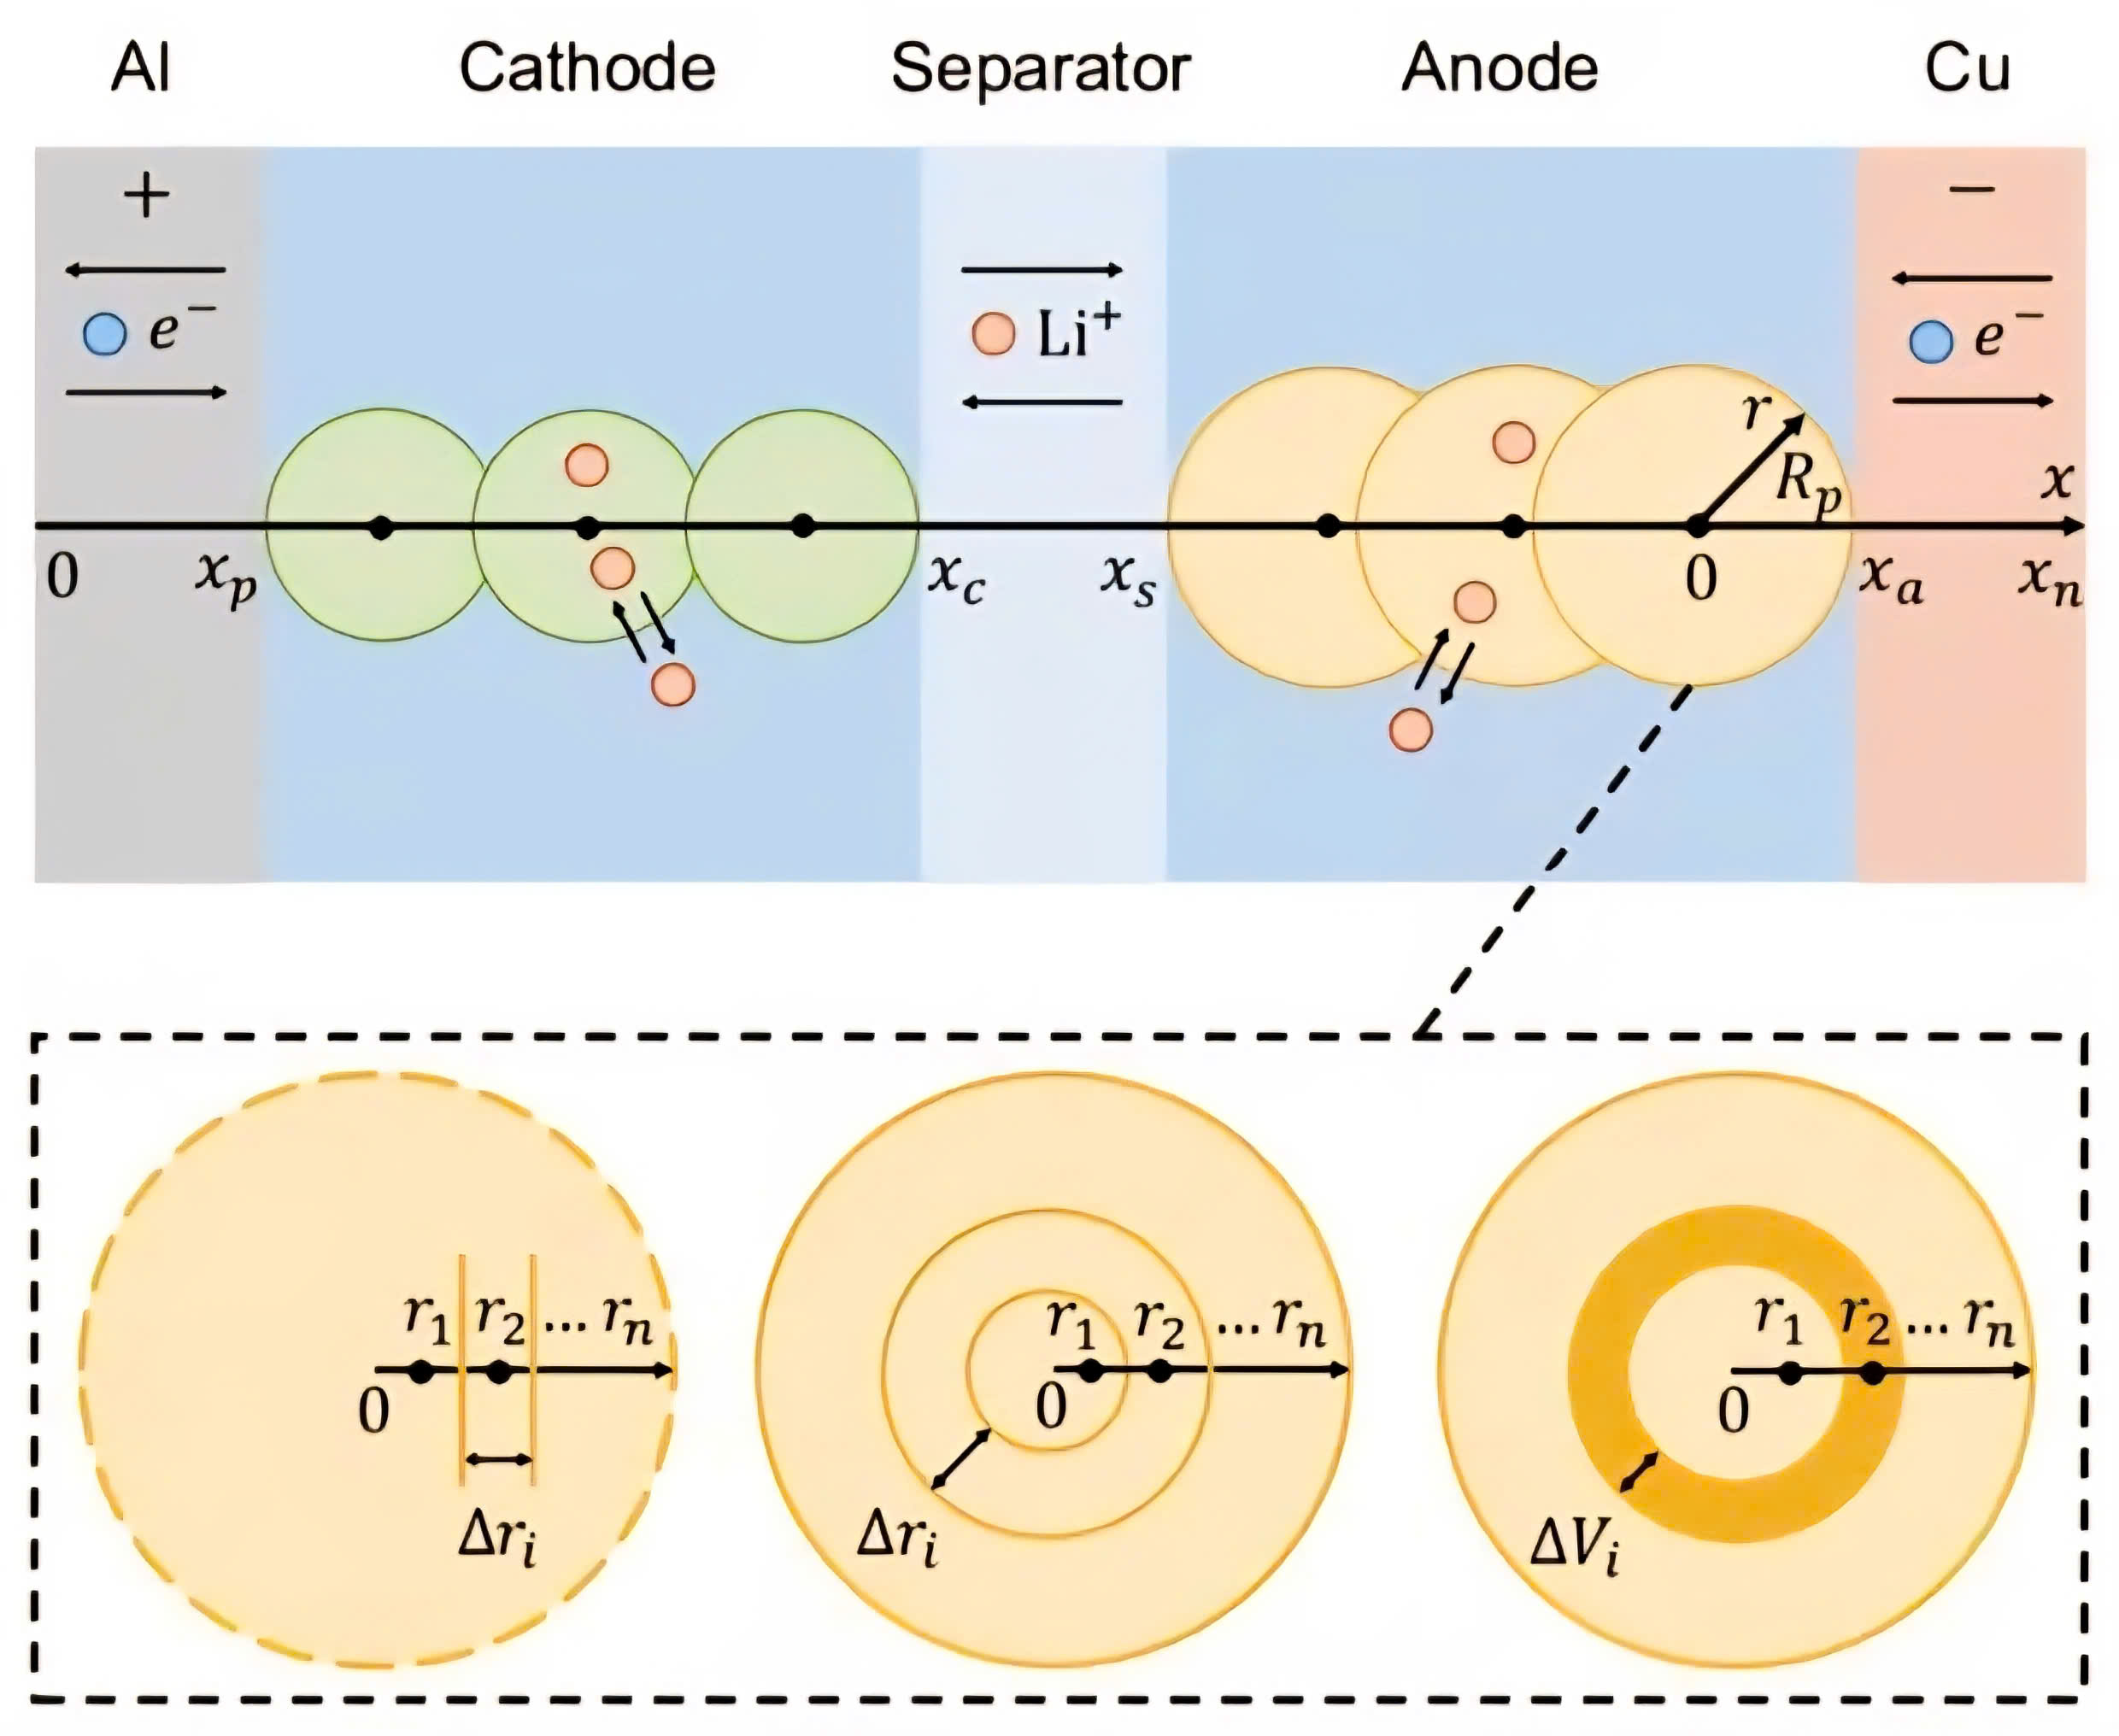
\includegraphics[width=0.8\textwidth]{media/image6.jpg}
        \caption{Mô hình P2D của pin}
        \label{fig:p2d}
    \end{figure}

  

    Nhằm cải thiện hiệu quả của mô hình SP khi dòng điện có biên độ lớn, mô hình SP mở rộng (ESP) đã được phát triển, đơn giản hóa các phương trình khuếch tán ion Li+ trong cả pha lỏng và pha rắn bằng phương pháp Parabol 3 tham số kết hợp với xấp xỉ Padé \cite{xin2020}. Mô hình ESP được đánh giá cao trong việc duy trì độ chính xác vốn có của mô hình SP đồng thời tăng khả năng thích ứng với dòng điện cao. Tuy nhiên, do vẫn phụ thuộc vào điều kiện dòng điện không đổi, mô hình ESP không phải là lựa chọn tối ưu cho việc nghiên cứu phương pháp sạc ổn dòng nhiều mức. Với mục tiêu khám phá đặc tính động của pin trong nhiều điều kiện dòng điện khác nhau và ứng dụng thời gian thực, các nhà nghiên cứu đã phát triển nhiều biến thể của mô hình SP2D bằng cách đơn giản hóa mô hình P2D theo những cách khác nhau. Trong số đó, nghiên cứu \cite{nejad2016} đề xuất một mô hình đa hạt đơn giản sử dụng thuật toán dự báo-thích nghi để cân bằng giữa độ chính xác và tính phức tạp của mô hình. Bằng cách xấp xỉ nồng độ dung dịch điện phân, thuật toán này giảm thiểu 22\% độ phức tạp của bài toán, đồng thời dự báo và thích ứng với các hiệu ứng không đồng đều trong phản ứng hóa học, từ đó cải thiện hiệu suất tính toán và độ chính xác ước lượng.

    \subsection{Mô hình mạch điện tương đương (ECM)}
    Mô hình điện hóa, tuy chính xác, nhưng lại khá phức tạp do sử dụng nhiều phương trình vi phân, đòi hỏi khả năng tính toán lớn và chứa nhiều tham số. Vì vậy, mô hình mạch tương đương được phát triển để đơn giản hóa việc nghiên cứu pin. Mô hình này mô phỏng hoạt động và đặc tính của pin bằng các thành phần điện cơ bản như điện trở, tụ điện và nguồn điện áp \cite{weiliu2022}. Nhờ cấu trúc đơn giản, dễ hiểu và ít tham số hơn mô hình điện hóa, mô hình mạch tương đương đã trở nên phổ biến trong cả nghiên cứu lý thuyết lẫn ứng dụng thực tế. Mô hình này được đánh giá cao về khả năng cân bằng giữa độ chính xác, độ phức tạp và tính ứng dụng, đồng thời có thể được điều chỉnh linh hoạt để phù hợp với các bài toán cụ thể.

    Mô hình đơn giản nhất là mô hình Rint (Hình \ref{fig:rint}) được cấu tạo bởi một nguồn áp lý tưởng và một nội trở mắc nối tiếp, các thành phần này đều thay đổi theo SoC và nhiệt độ của pin.

    \begin{figure}[H]
        \centering
        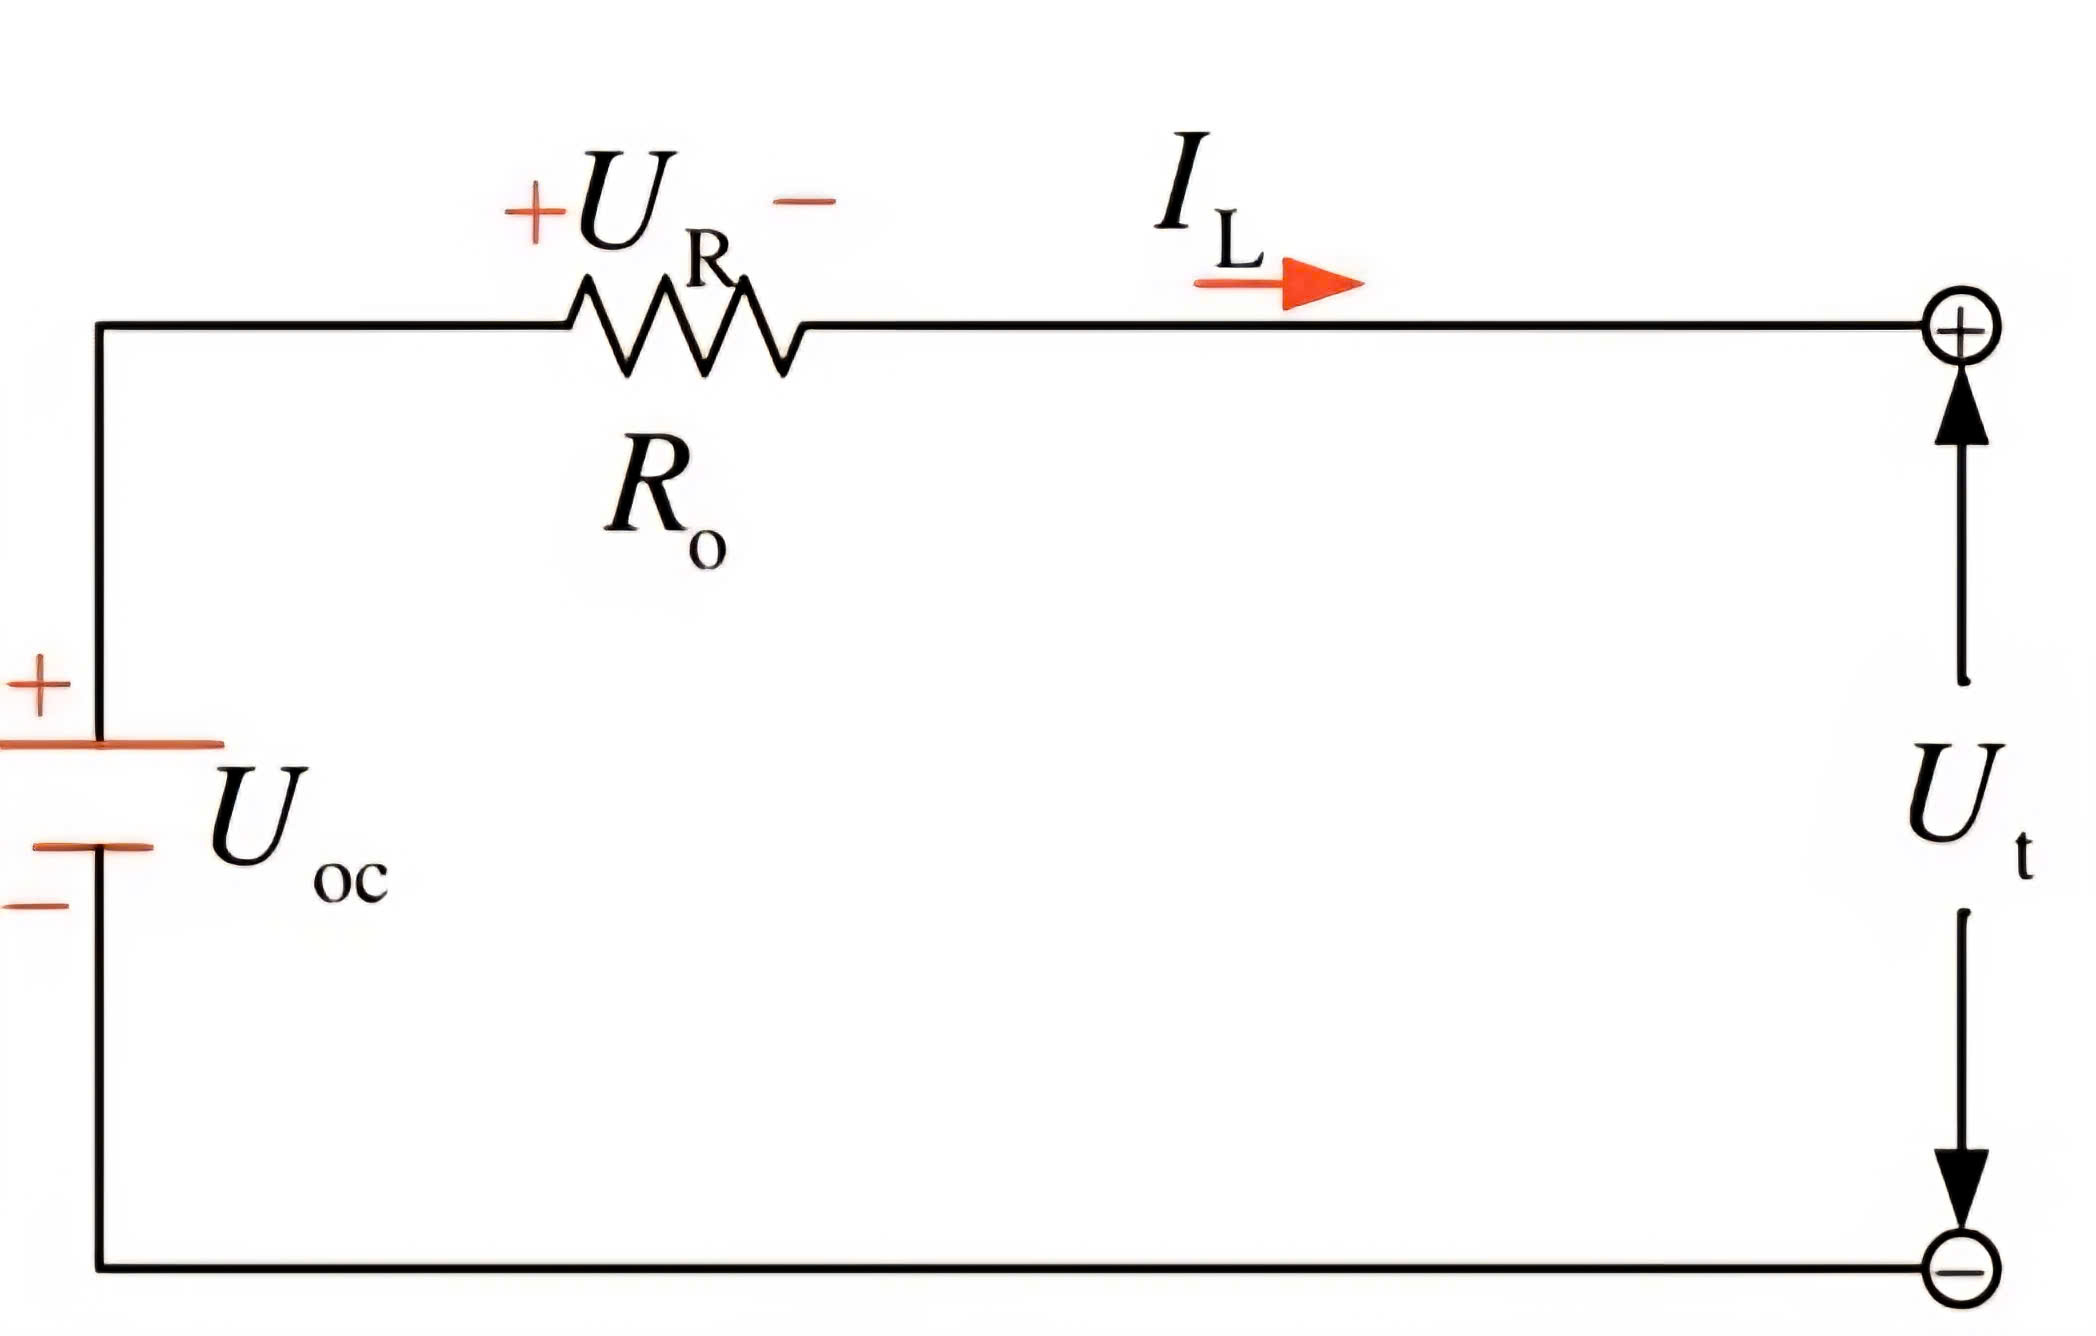
\includegraphics[width=0.5\textwidth]{media/image7.jpg}
        \caption{Mô hình Rint}
        \label{fig:rint}
    \end{figure}

    Tuy nhiên, mô hình này chưa phản ánh được đặc tính động (hiện tượng phân cực) trong quá trình hoạt động của pin nên chỉ phù hợp với các ứng dụng đơn giản, không đòi hỏi độ chính xác cao \cite{weiliu2022}. Hiện tượng phân cực thường xuất hiện khi dòng điện chạy qua pin, gây ra các cản trở trong việc di chuyển ion và electron, cũng như các phản ứng hóa học tại bề mặt điện cực. Hiện tượng phân cực thể hiện rõ nhất khi có sự chênh lệch giữa điện áp thực tế tại đầu cực của pin (điện áp đầu cuối) và điện áp lý tưởng của pin (điện áp mạch hở - $U_{oc}$) mặc dù pin không trong quá trình sạc hoặc xả. Lúc này, pin vừa được sạc hoặc xả, điện áp trên pin không lập tức trở về $U_{oc}$ mà từ từ tăng (giảm) về $U_{oc}$ (Hình \ref{fig:phancuc}). \cite{plett2015}

    \begin{figure}[H]
        \centering
        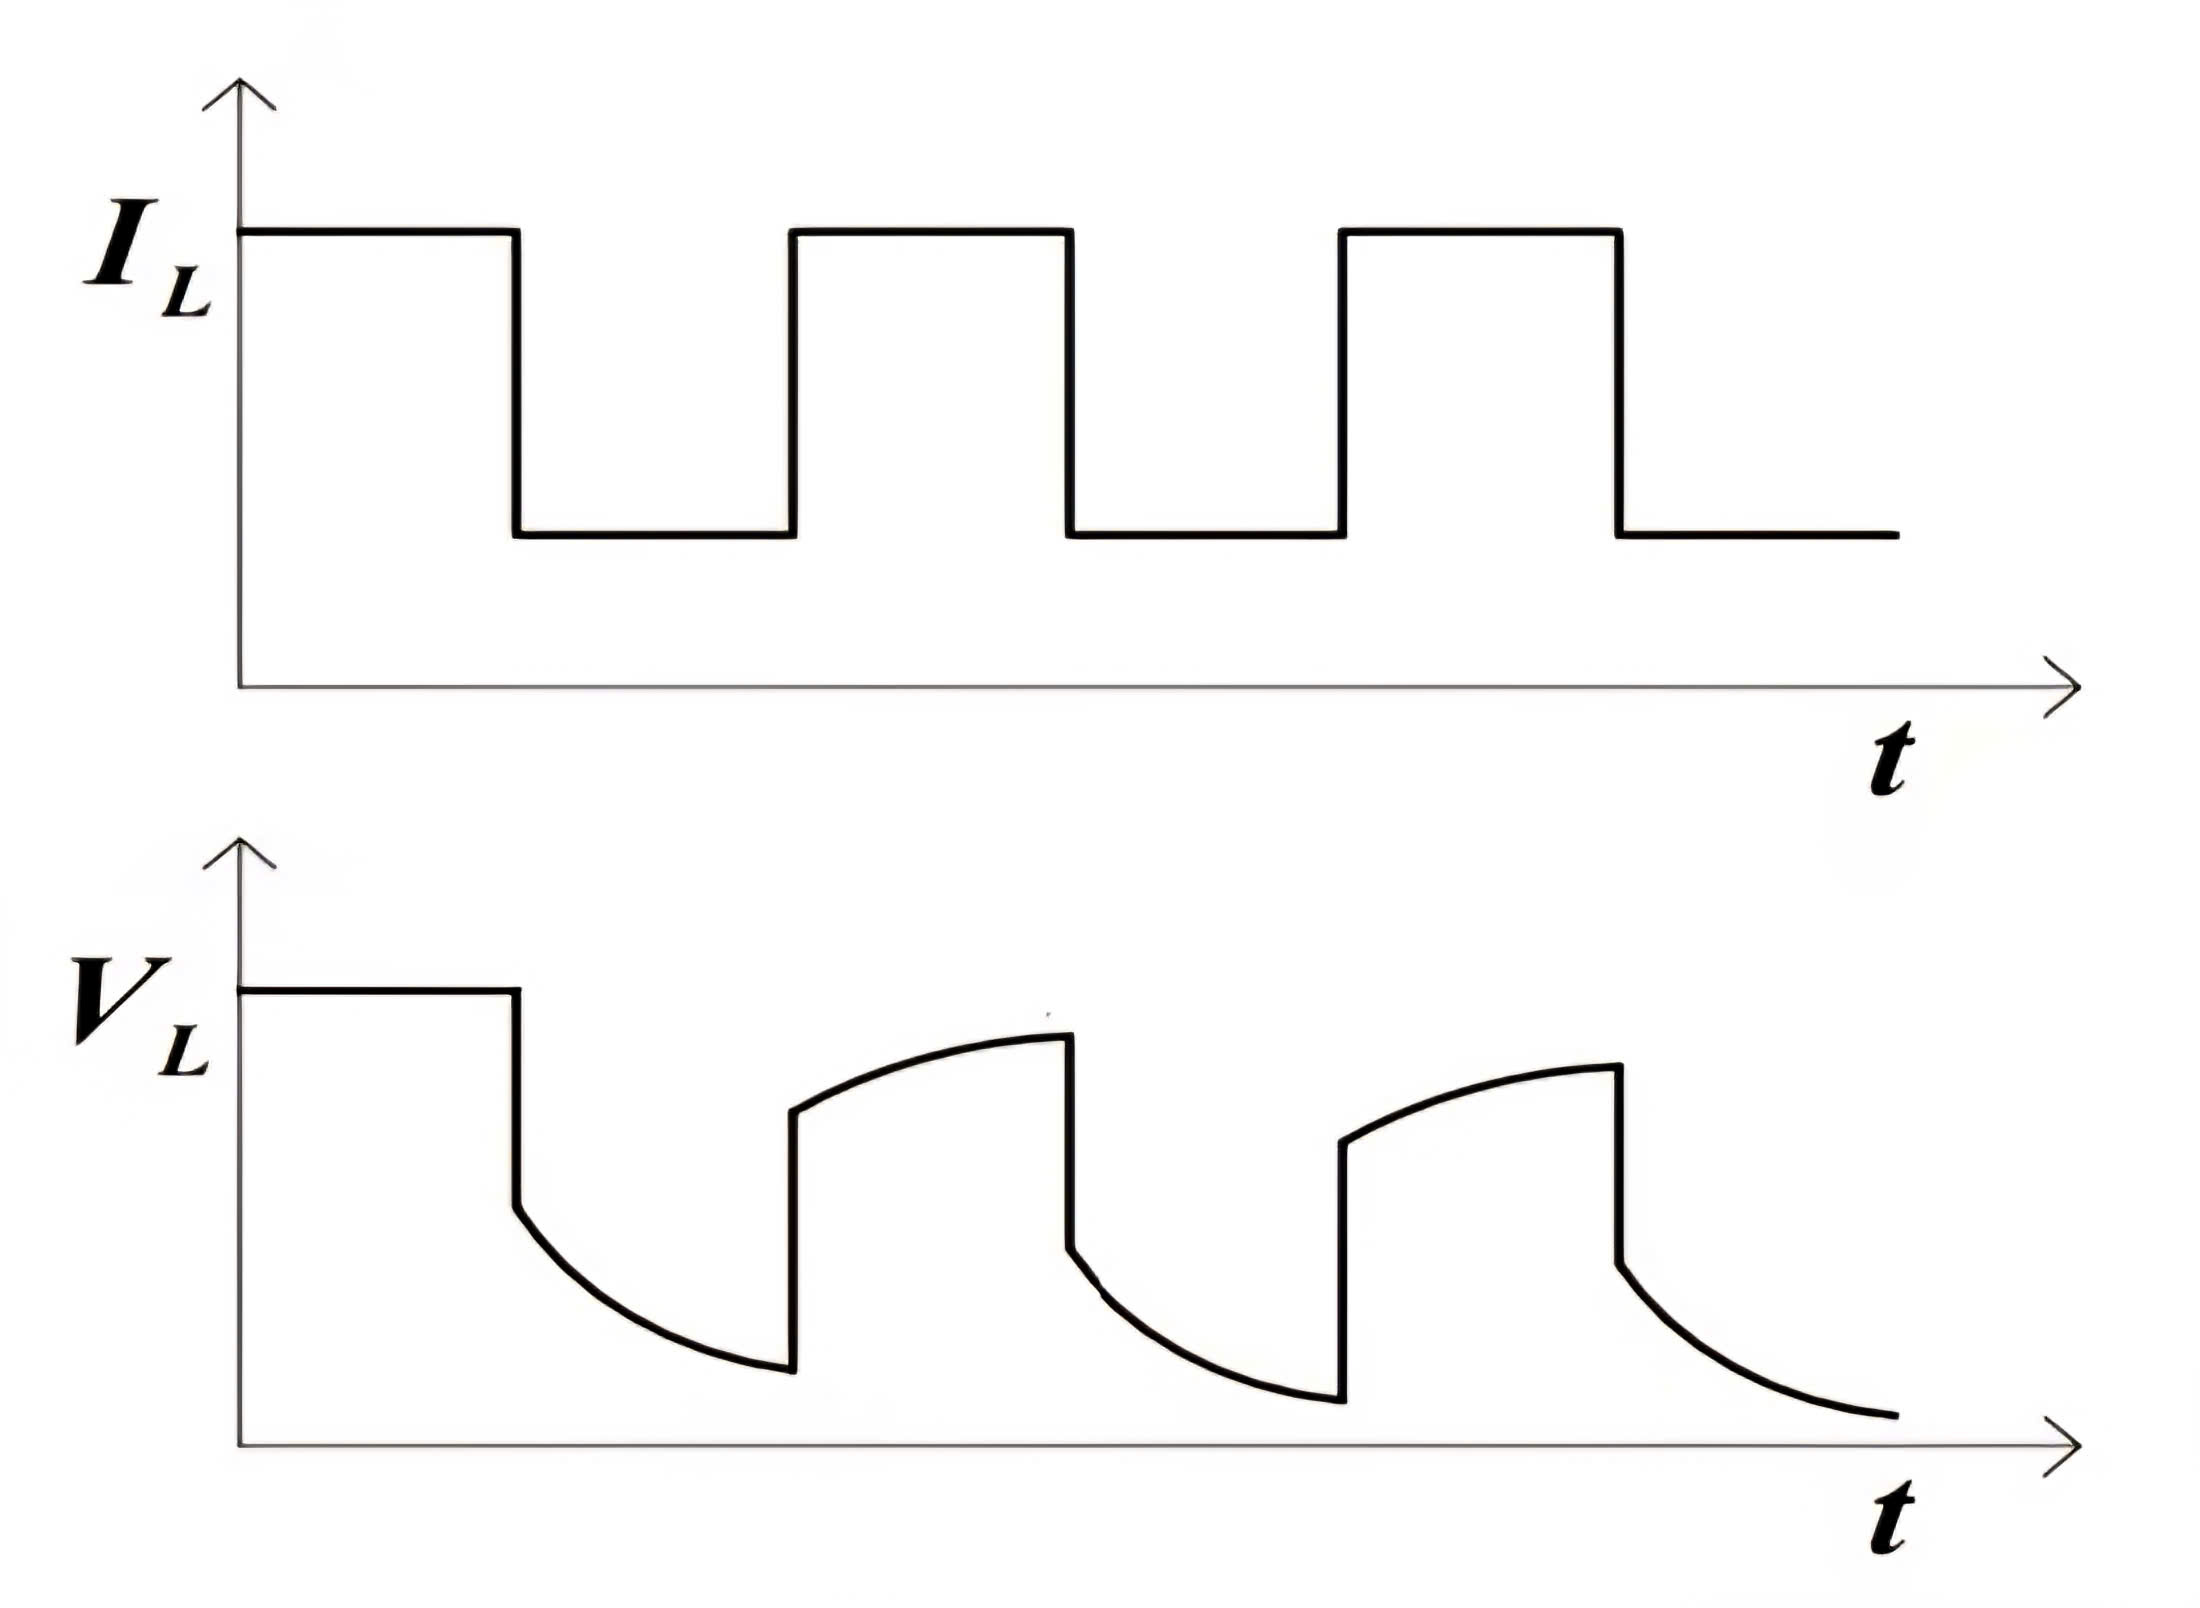
\includegraphics[width=0.8\textwidth]{media/image8.jpg}
        \caption{Điện áp trên pin khi có các xung xả}
        \label{fig:phancuc}
    \end{figure}

    Do đó, mô hình Thevenin ra đời bằng cách thêm mạng RC song song vào mô hình Rint (Hình \ref{fig:thevenin}) mang lại độ chính xác cao hơn và khả năng mô tả hiện tượng phân cực bên trong pin. Mô hình này sử dụng nội trở $R_0$ để biểu diễn sự thay đổi điện áp đột ngột và $R_p$, $C_p$ để thể hiện sự thay đổi điện áp từ từ khi pin sạc/xả \cite{campagna2020}.

    \begin{figure}[H]
        \centering
        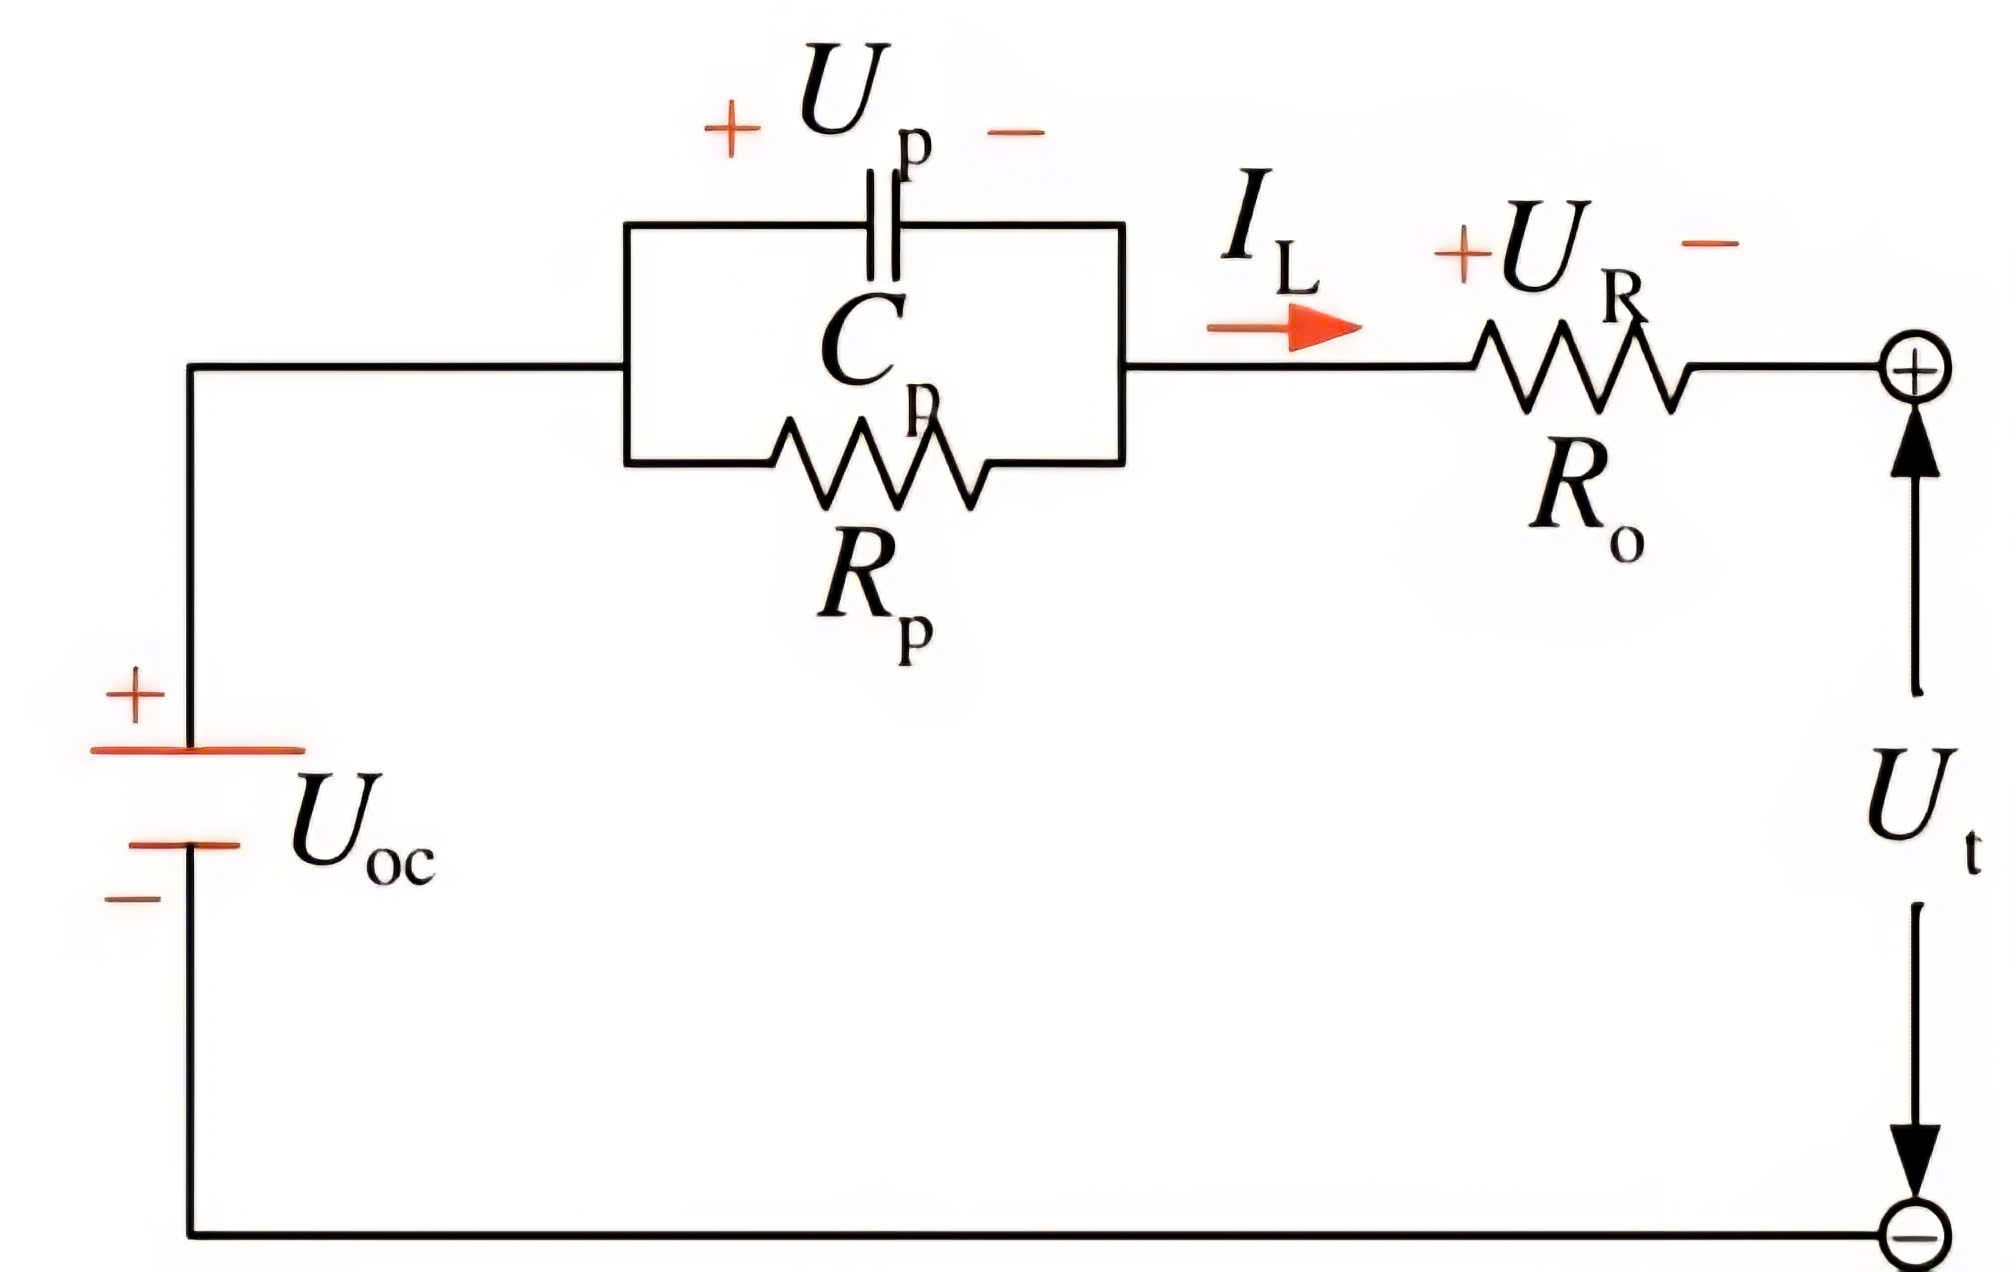
\includegraphics[width=0.5\textwidth]{media/image9.jpg}
        \caption{Mô hình Thevenin}
        \label{fig:thevenin}
    \end{figure}

    Ngoài ra, các nghiên cứu còn chỉ ra rằng khi càng có thêm nhiều nhánh RC thì độ chính xác của mô hình càng tăng lên, điều này là do hiện tượng phân cực lại được chia thành nhiều loại như phân cực nồng độ, phân cực điện hóa,… thời gian xảy ra của mỗi loại phân cực là khác nhau nên do đó mỗi nhánh RC sẽ phản ánh cho mỗi loại phân cực này. Hình \ref{fig:dp} mô tả mô hình bậc 2 (gồm 2 nhánh RC), hay còn gọi là mô hình DP (Dual Polarization), mô hình này đã có thể phản ánh hai hiện tượng phân cực điển hình là phân cực điện hóa và nồng độ \cite{zhang2010}.

    \begin{figure}[H]
        \centering
        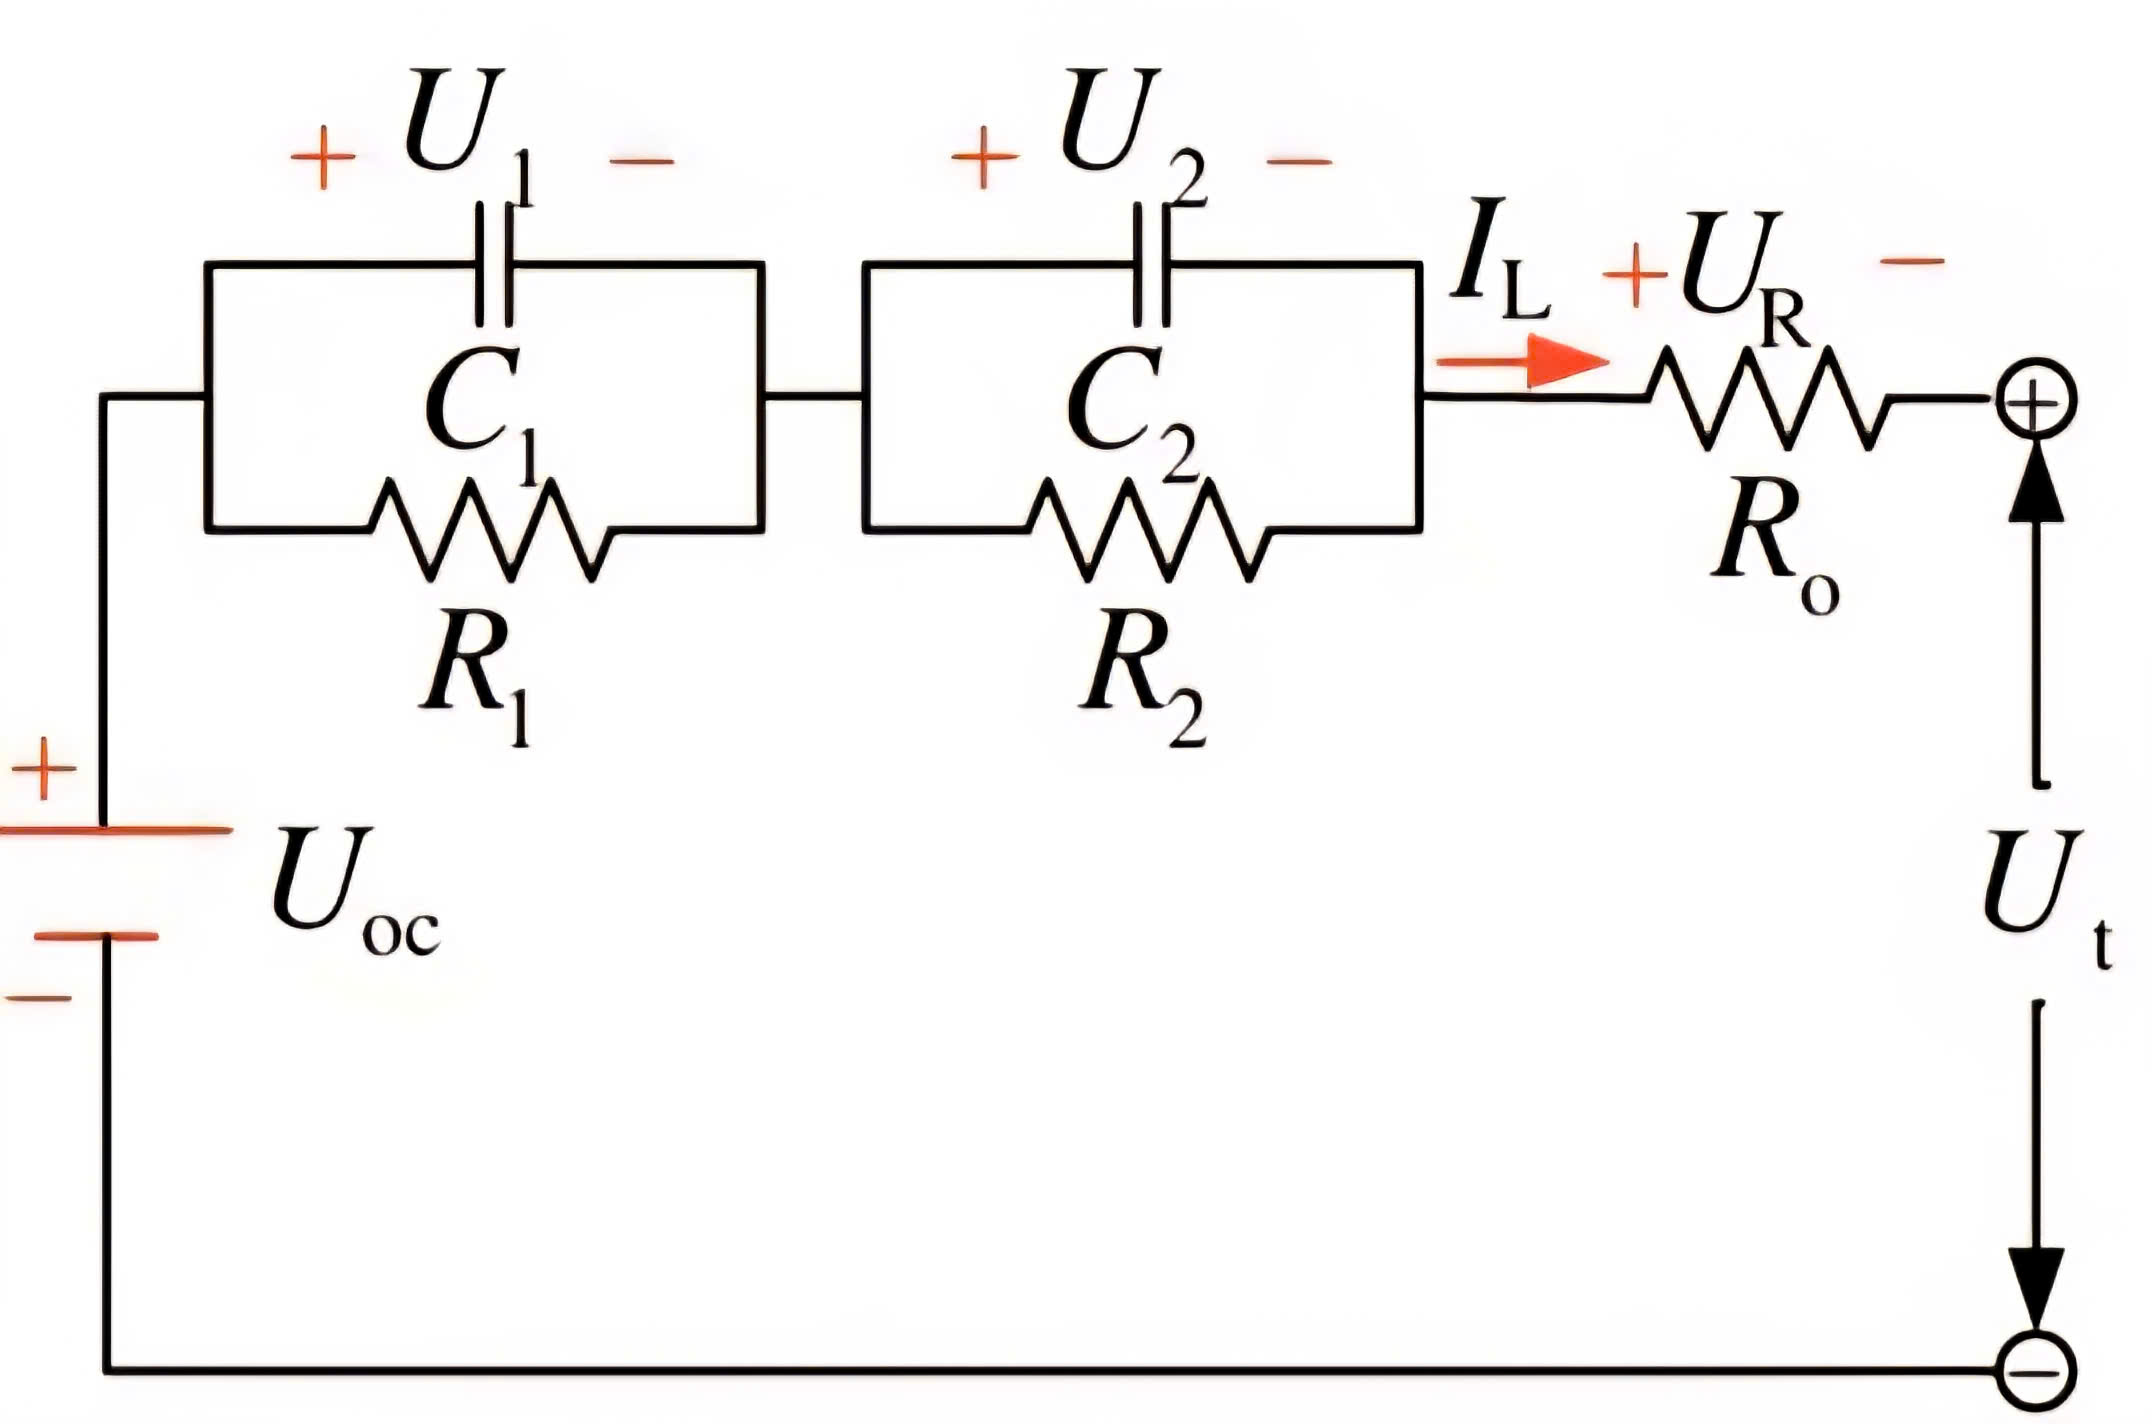
\includegraphics[width=0.5\textwidth]{media/image10.jpg}
        \caption{Mô hình DP}
        \label{fig:dp}
    \end{figure}

    Đồ án này sẽ tiến hành so sánh ba loại mô hình mạch điện tương đương phổ biến Rint, Thevenin và DP được đề cập bên trên về tiêu chí là độ chính xác.
\newpage
    \section*{CHƯƠNG 3. PHƯƠNG PHÁP XÁC ĐỊNH THÔNG SỐ MÔ HÌNH}
    \addcontentsline{toc}{section}{\numberline{} CHƯƠNG 3. PHƯƠNG PHÁP XÁC ĐỊNH THÔNG SỐ MÔ HÌNH}
    \setcounter{section}{3}
    \setcounter{subsection}{0}
    \setcounter{figure}{0}
    \setcounter{table}{0}

    Việc xác định chính xác thông số mô hình mạch điện tương đương (nguồn áp, điện trở, tụ điện) là vô cùng quan trọng, ảnh hưởng đáng kể đến tính chính xác của mô hình.

    \subsection{Bài thí nghiệm HPPC xây dựng mô hình pin}
    \subsubsection{Cơ sở lý thuyết bài thí nghiệm HPPC xây dựng mô hình pin}
    Trong nhiều bài nghiên cứu về pin, mô hình pin và các ứng dụng thời gian thực, các phương pháp thường dùng bao gồm: sử dụng phổ trở kháng điện hóa (Electrochemical Impedance Spectroscopy - EIS) và bài thí nghiệm đặc tính theo xung lai (Hybrid Pulse Power Characterization - HPPC). EIS là một phương pháp ưu tiên việc sử dụng công cụ, máy móc; các công cụ vẫn có giá thành đáng kể \cite{macdonald2006}. Một phương án hợp lý, phù hợp hơn với quy mô phòng thí nghiệm và phạm vi, nội dung của đồ án là phương pháp sử dụng bài thí nghiệm HPPC. Đây là phương pháp áp dụng các xung sạc/xả với thời gian ngắn (được gọi là chu trình HPPC) để quan sát đặc tính động của pin.
    
    Xét tại 1 chu trình HPPC, tức tại 1 giá trị SoC khởi điểm, dạng đồ thị dòng điện, điện áp cho các xung sạc/xả/nghỉ thời gian ngắn được cho trong Hình \ref{fig:hppc_graph}.

    \begin{figure}[H]
        \centering
        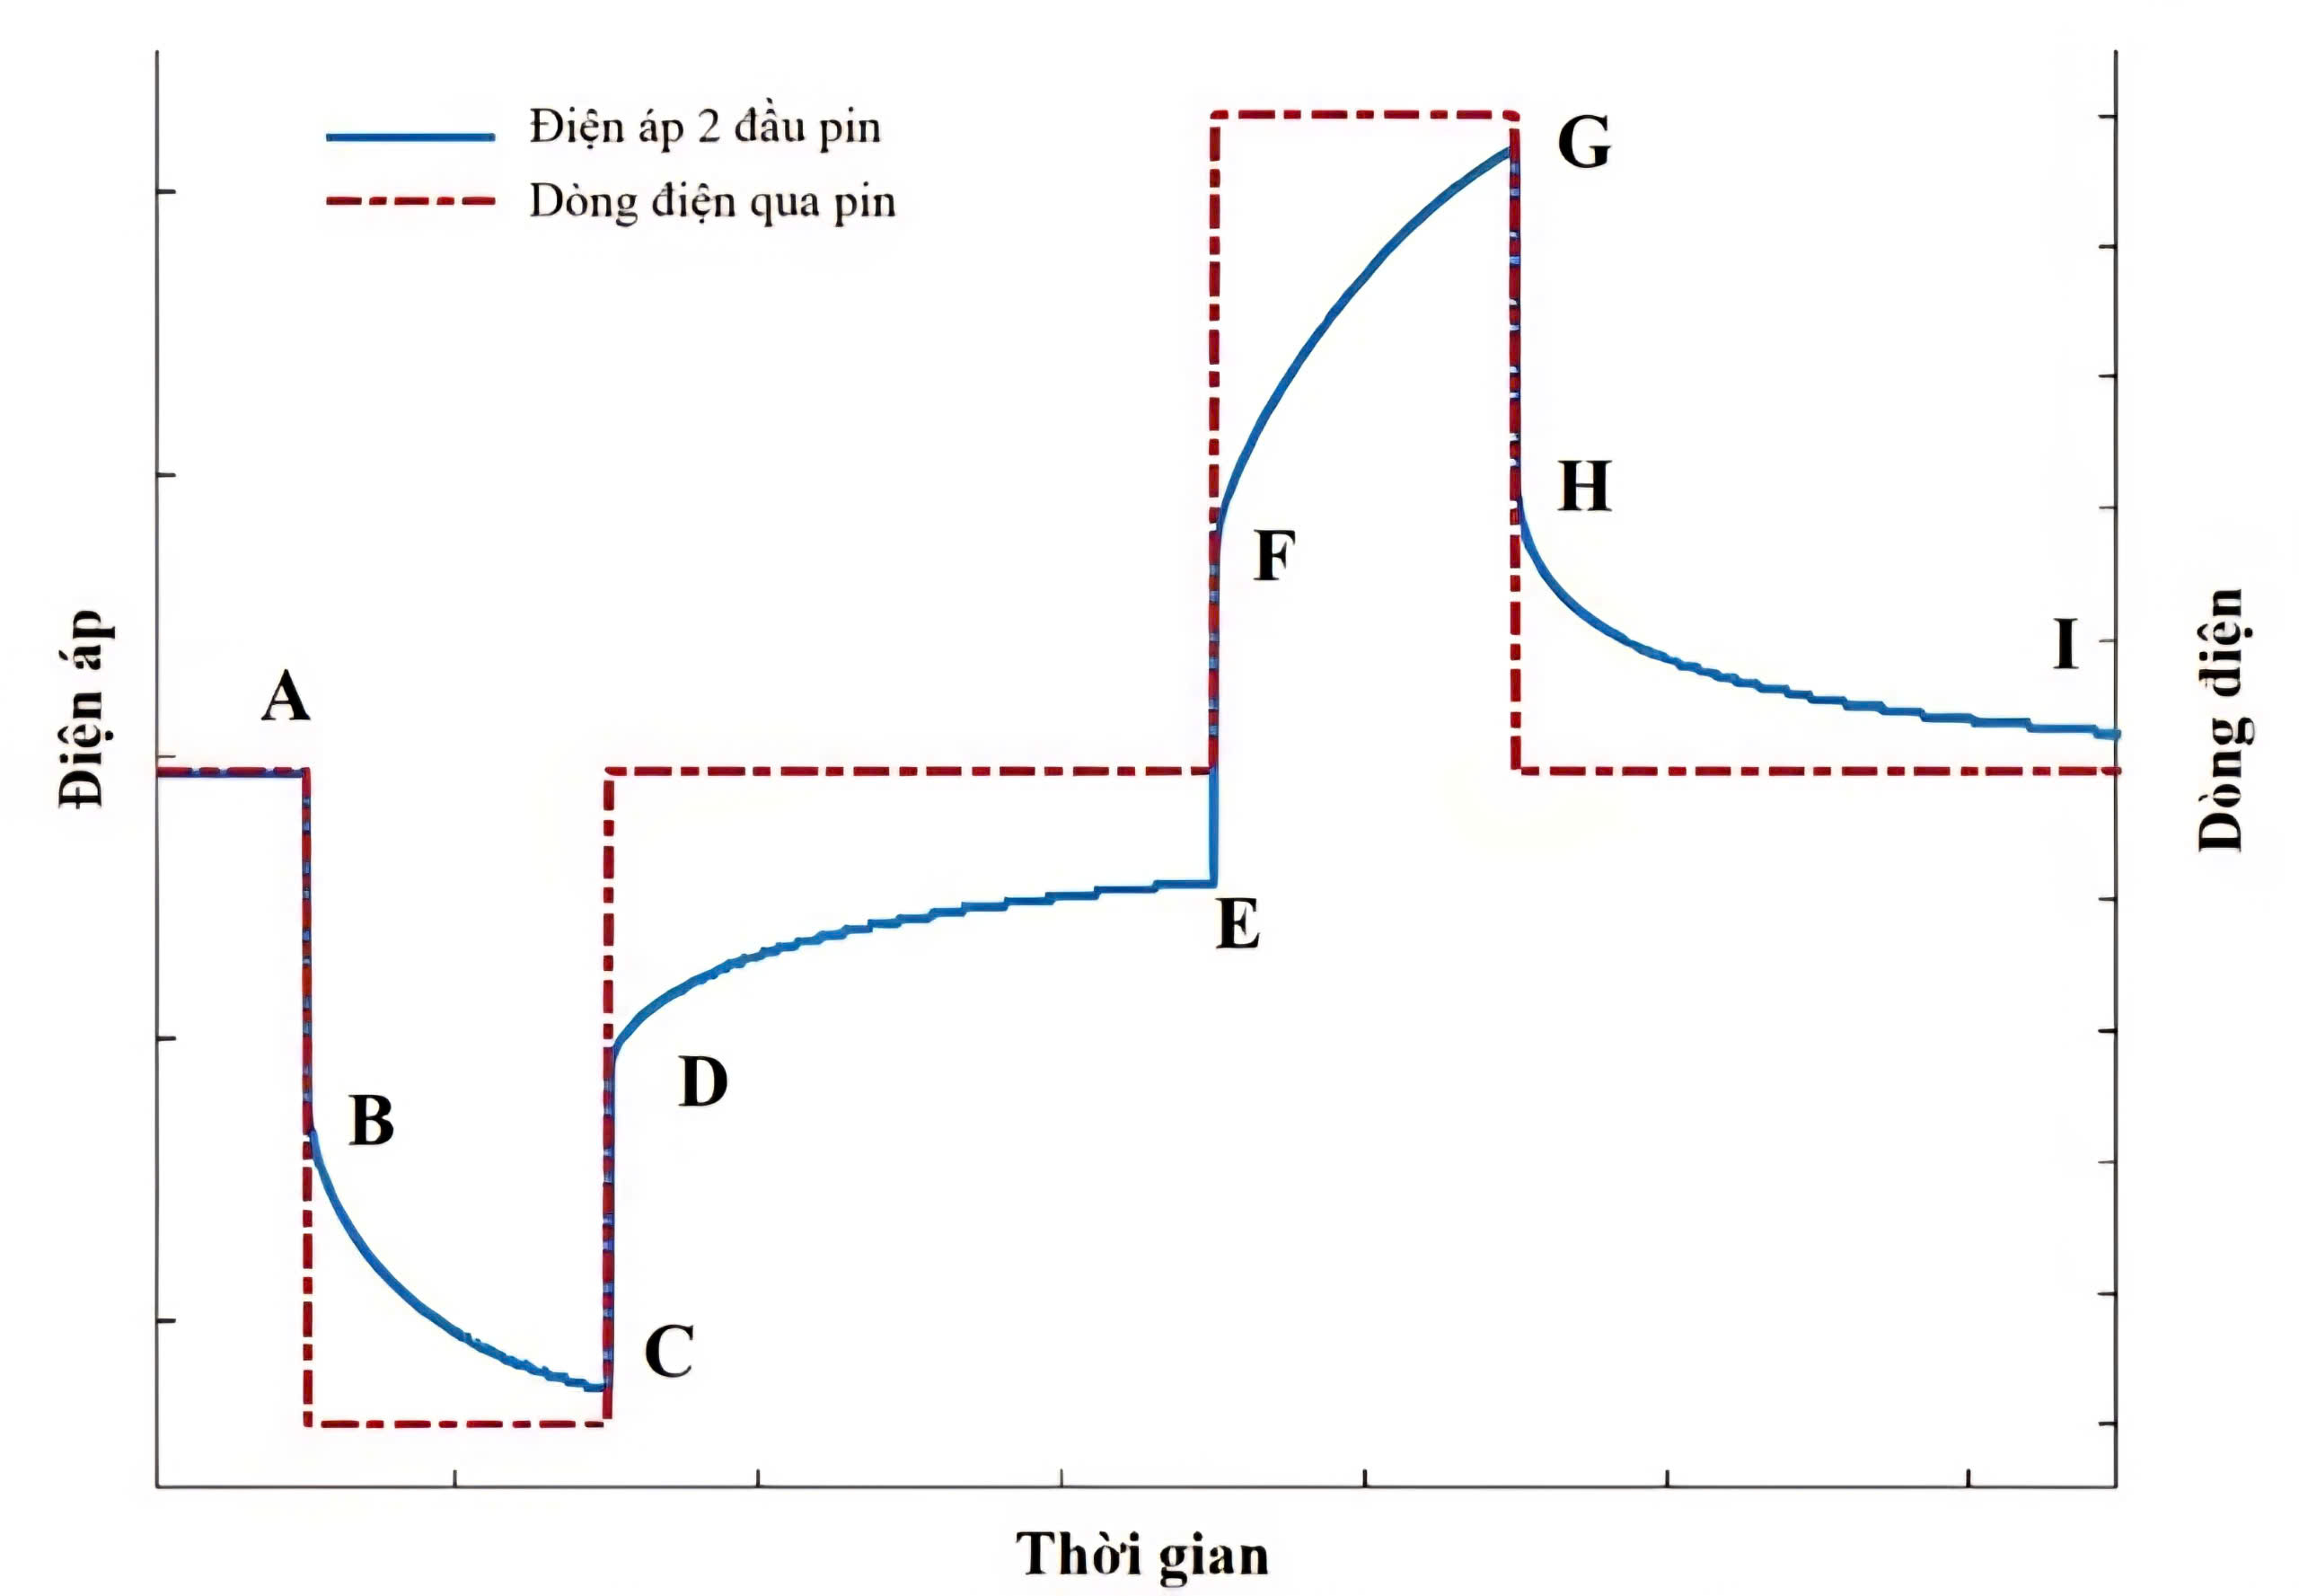
\includegraphics[width=0.8\textwidth]{media/image12.jpg}
        \caption{Đồ thị dòng điện, điện áp trong 1 chu trình HPPC}
        \label{fig:hppc_graph}
    \end{figure}

        Dựa vào đồ thị này, các phương pháp xác định thông số của từng mô hình mạch điện tương đương sẽ được trình bày ở mục 3.2. Do phạm vi đồ án, các mô hình được phục vụ cho quá trình sạc CC-CV nên mô hình sạc của pin sẽ được xác định dựa vào đoạn đồ thị từ thời điểm $t_E$ đến $t_I$, trong phạm vi rộng hơn. Mô hình xả của pin cũng được xác định bằng phương pháp tương tự. Để đơn giản hóa các tính toán, biểu diễn, thời điểm ban đầu $t_E = t_F$ sẽ được tạm dịch về 0.
    \subsubsection{Quy trình bài thí nghiệm HPPC}
    Hình \ref{fig:hppc} mô tả sơ lược quy trình thực hiện bài thí nghiệm HPPC, các bước lần lượt như sau:

    \begin{itemize}
        \item Sạc CC-CV đầy pin, tùy thuộc mức dòng sạc, giá trị SoC khởi điểm và khuyến nghị của NSX.
        \item Sau khi sạc đầy pin thì ngắt sạc, cho pin nghỉ với thời gian đủ lâu. Mục tiêu của việc cho nghỉ sau sạc là để điện áp trên 2 đầu pin trở về xấp xỉ điện áp hở mạch của pin (điện áp hở mạch có liên hệ với SoC). Thời gian nghỉ này có thể kéo dài đến 1 giờ (tùy thuộc khuyến nghị của NSX).
        \item Tiến hành đo giá trị điện áp 2 đầu pin sau thời điểm nghỉ, giá trị này tương đương với điện áp hở mạch của pin khi SoC đạt 100\%.
        \item Bắt đầu thực hiện 1 chu trình HPPC, bước đầu tiên là xả pin với 1 mức dòng trong thời gian ngắn. Mức dòng và khoảng thời gian ngắn này được lựa chọn để đảm bảo SoC của pin không bị suy giảm đáng kể (tức $U_{oc}$ coi như không đổi). Trong các nghiên cứu và hướng dẫn về HPPC \cite{idaho2020}, mức dòng xả được chọn là 1C và thời gian xả là 30 giây.
        \item Sau khi thực hiện xả, tiến hành cho pin nghỉ trong khoảng thời gian ngắn (khoảng vài chục giây). Trong các nghiên cứu và hướng dẫn về HPPC \cite{idaho2020}, thời gian nghỉ thường được chọn trong khoảng 40 giây.
        \item Tiến hành sạc pin với mức dòng tương đương khi xả ở bước 1, trong khoảng thời gian tương đương. Sau đó, pin cũng được cho nghỉ trong khoảng thời gian tương tự bước 2.
    \end{itemize}

    \begin{figure}[H]
        \centering
        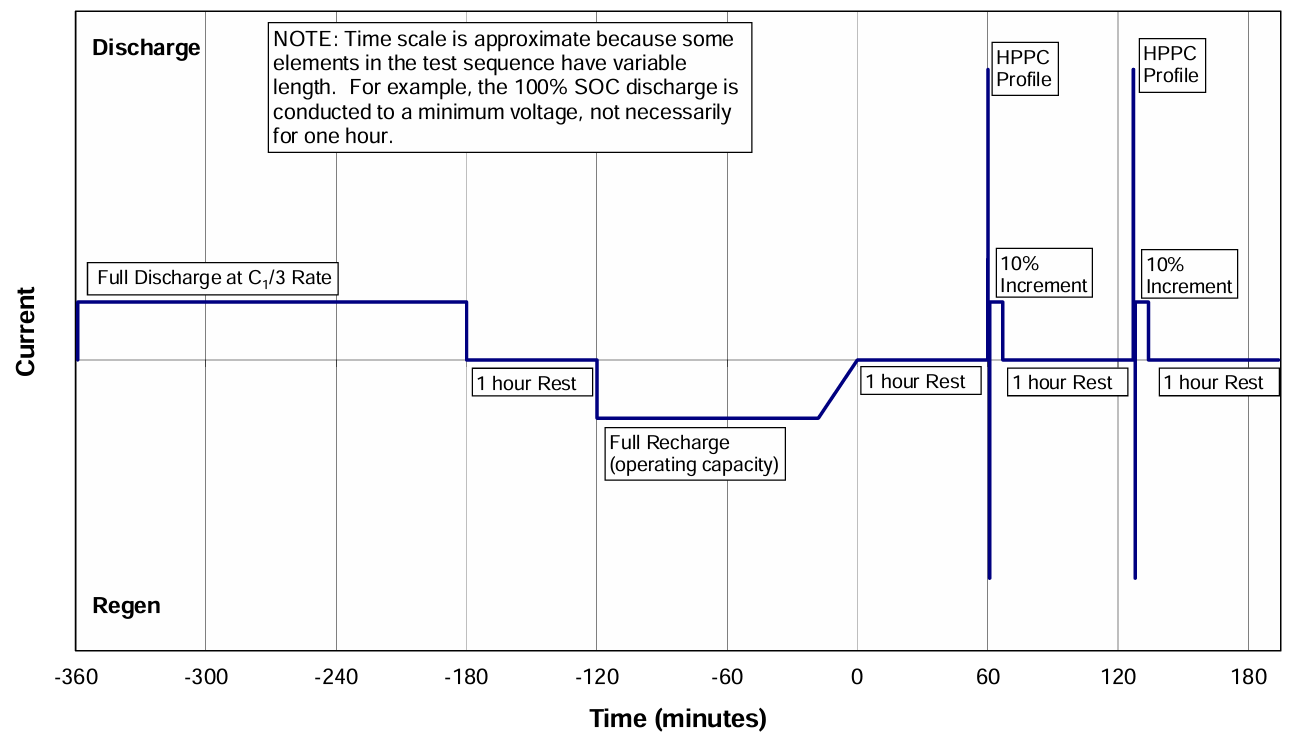
\includegraphics[width=0.8\textwidth]{media/image11.png}
        \caption{Quy trình bài thí nghiệm HPPC}
        \label{fig:hppc}
    \end{figure}

    
\subsection{Các phương pháp xác định mô hình điện tương đương cho Pin}
    \subsubsection{Phương pháp xác định mô hình Rint}
    Tại thời điểm ban đầu $t_E$, pin đã được nghỉ đủ lâu để hiện tượng phân cực kết thúc. Nguồn áp $U_{oc}$ được xác định bằng cách đo điện áp tại $E$. Khi đó:
\begin{equation}
U_{oc} = V_E 
\end{equation}
    Khi pin bắt đầu giai đoạn sạc, điện áp 2 đầu tại $E$ và $F$ thay đổi lập tức 1 lượng do nội trở $R_0$. Tương tự, khi pin kết thúc giai đoạn xả, điện áp 2 đầu tại $G$ và $H$ thay đổi lập tức 1 lượng do nội trở $R_0$. Ta có:

    \begin{equation}
V_F - V_E = V_G - V_H = I \cdot R_0 
\end{equation}

    Như vậy, nội trở $R_0$ có thể được tính theo công thức sau:

    \begin{equation}
R_0 = \frac{(V_F - V_E) + (V_G - V_H)}{2I} 
\end{equation}

    Phép lấy trung bình 2 biểu thức là để tăng tính chính xác và bù các sai lệch do quá trình sạc pin gây ra với điện áp 2 đầu cực.

    \subsubsection{Phương pháp xác định mô hình Thevenin}
    Nguồn áp $U_{oc}$ và nội trở $R_0$ được xác định tương tự như phương pháp trên. Đối với 2 giá trị điện trở và tụ điện phân cực, cần kết hợp giải quyết dựa trên 2 giai đoạn khi sạc pin từ $F$ đến $G$ và khi cho pin nghỉ từ $H$ đến $I$. Theo định luật Kirchhoff và các định luật cơ bản trong mạch điện, có:

    \begin{itemize}
        \item Khi pin sạc trong khoảng thời gian từ $F$ đến $G$:
    \end{itemize}

    \begin{equation}
\begin{cases}
i = i_{Rp} + i_{Cp} \\
u_p = i_{Rp} \cdot R_p\\
i_{Cp} = C_p \cdot \frac{du_p}{dt}\\
u_t = u_{oc} + i \cdot R_0 + u_p  \\ 
\end{cases}
\end{equation}

    Trong đó: $u_{oc}$, $u_p$, $u_t$, $i$, $i_{Rp}$, $i_{Cp}$ lần lượt là giá trị tức thời của điện áp hở mạch, điện áp phân cực, điện áp 2 đầu pin, dòng điện qua pin, dòng điện qua $R_p$ và dòng điện qua $C_p$.

    Từ 3 phương trình đầu trong hệ, có:

    \begin{equation}
\frac{du_p(t)}{dt} + \frac{u_p(t)}{C_p R_p} = \frac{i}{C_p} 
\end{equation}


    Đây là phương trình vi phân thuần nhất, giải phương trình vi phân này ta được:

    \begin{equation}
u_p = i \cdot R_p + (u_p(0) - i \cdot R_p) \cdot e^{-\frac{t}{R_p \cdot C_p}} 
\end{equation}

    Xét điều kiện đầu, tức tại $t=0$, điện áp phân cực trên pin có giá trị bằng 0, hay $u_p(0) = 0$. Ta có tại thời điểm $G$, phương trình trên trở thành:

   \begin{equation}
u_p(t_G) = i \cdot R_p + (-i \cdot R_p) \cdot e^{-\frac{t_G}{R_p \cdot C_p}} 
\end{equation}

    Suy ra, điện trở phân cực:

    \begin{equation}
R_p = \frac{u_p(t_G)}{i \cdot (1 - e^{-\frac{t_G}{R_p \cdot C_p}})} 
\end{equation}

    Do \( u_p(t_G) = V_G - V_F \), suy ra:

    \begin{equation}
R_p = \frac{V_G - V_F}{i \cdot (1 - e^{-\frac{t_G}{R_p \cdot C_p}})} 
\end{equation}

\begin{itemize}
    \item Khi pin nghỉ trong khoảng thời gian từ \( H \) đến \( I \):
\end{itemize}

Lúc này, tụ \( C_p \) sẽ xả qua trở \( R_p \). Ta có:

\begin{equation}
u_p = i \cdot R_p = \frac{q_p}{C_p} 
\end{equation}

Đạo hàm hai vế, ta được:

\begin{equation}
\frac{d(i \cdot R_p)}{dt} = \frac{dq_p}{C_p \, dt} = -\frac{i}{C_p} 
\end{equation}

Chuyển vế:

\begin{equation}
\frac{di}{i} = -\frac{dt}{R_p C_p} 
\end{equation}

Nhân vế trái với \( R_p \):

\begin{equation}
\frac{du_p}{u_p} = -\frac{dt}{R_p C_p} 
\end{equation}

Tích phân hai vế từ thời điểm \( t_H \) đến thời điểm \( t_K \) (là thời điểm thỏa mãn \( t_H < t_K < t_I \)), ta được:

\begin{equation}
\ln\left(\frac{u_p(t_K)}{u_p(t_H)}\right) = -\frac{t_K - t_H}{R_p C_p} 
\end{equation}

Suy ra:

\begin{equation}
u_p(t_K) = u_p(t_H) \cdot e^{-\frac{t_K - t_H}{R_p C_p}} 
\end{equation}

Ta có: \( u_p(t_H) = V_G - V_F \), suy ra:

\begin{equation}
u_p(t_K) = (V_G - V_F) \cdot e^{-\frac{t_K - t_H}{R_p C_p}} 
\end{equation}

Xét phương trình Kirchhoff: \( u_t = u_{oc} + i R_0 + u_p \). Tại thời điểm \( t_K \), thay \( i = 0 \), \( u_p(t_K) = (V_G - V_F) \cdot e^{-\frac{t_K - t_H}{R_p C_p}} \), vì sạc trong thời gian ngắn nên coi \( u_{oc} \) không đổi trong suốt chu trình HPPC và bằng \( V_E \), do đó:

\begin{equation}
u_t(t_K) = V_E + (V_G - V_F) \cdot e^{-\frac{t_K - t_H}{R_p C_p}} 
\end{equation}

Suy ra:

\begin{equation}
R_p C_p = -\frac{t_K - t_H}{\ln\left(\frac{V_K - V_E}{V_G - V_F}\right)} 
\end{equation}

Kết hợp với phương trình (2.9), giải hệ phương trình hai ẩn, ta xác định được \( R_p \) và \( C_p \) của mô hình Thevenin.

\subsubsection{Phương pháp xác định mô hình DP}
Nguồn áp \( u_{oc} \) và nội trở \( R_0 \) của mô hình DP vẫn được xác định tương tự như trên. Tuy nhiên, mô hình DP có thêm một nhánh \( R \), \( C \) mắc song song so với mô hình Thevenin, vì vậy đòi hỏi một phương pháp khác để xác định điện trở và tụ điện phân cực \( R_1 \), \( R_2 \), \( C_1 \), \( C_2 \) của mô hình này.

Vẫn xét đồ thị một chu trình HPPC và kết hợp định luật Kirchhoff và các định luật cơ bản trong mạch điện, ta có:

\begin{itemize}
    \item Khi pin sạc trong khoảng thời gian từ \( F \) đến \( G \), tương tự như phương pháp xác định mô hình Thevenin:
\end{itemize}

\begin{equation}
R_1 = \frac{u_1(t_G)}{i \cdot (1 - e^{-\frac{t_G}{R_1 \cdot C_1}})} 
\end{equation}

\begin{equation}
R_2 = \frac{u_2(t_G)}{i \cdot (1 - e^{-\frac{t_G}{R_2 \cdot C_2}})} 
\end{equation}

\begin{itemize}
    \item Khi pin nghỉ trong khoảng thời gian từ \( H \) đến \( I \), tương tự như phương pháp xác định mô hình Thevenin, ta có phương trình tại thời điểm \( K \):
\end{itemize}

\begin{equation}
u_t(t_K) = V_E + u_1(t_G) \cdot e^{-\frac{t_K - t_H}{R_1 C_1}} + u_2(t_G) \cdot e^{-\frac{t_K - t_H}{R_2 C_2}} 
\end{equation}

Do \( u_1(t_G) + u_2(t_G) = V_G - V_F \), suy ra:

\begin{equation}
u_t(t_K) = V_E + u_1(t_G) \cdot e^{-\frac{t_K - t_H}{R_1 C_1}} + (V_G - V_F - u_1(t_G)) \cdot e^{-\frac{t_K - t_H}{R_2 C_2}} 
\end{equation}

So sánh phương trình (2.22) với phương trình (2.15) của phương pháp xác định mô hình Thevenin, ta thấy phương trình này có thêm \( u_1(t_G) \) là đại lượng không xác định được bằng cách đo lường. Do đó, không thể rút các điện trở và tụ điện phân cực ra để tính như phương pháp trước. Đồ án này trình bày phương pháp sử dụng Curve fitting của phần mềm Matlab để khớp đường cong của phương trình trên, từ đó xác định các tham số chưa biết là \( u_1(t_G) \), \( R_1 C_1 \) và \( R_2 C_2 \). Đầu tiên, đặt \( u_1(t_G) = k \), \( \frac{1}{R_1 C_1} = a \) và \( \frac{1}{R_2 C_2} = b \), thay vào phương trình (2.22) ta được:

\begin{equation}
u_t(t_K) = V_E + k \cdot e^{-\frac{t_K - t_H}{a}} + (V_G - V_F - k) \cdot e^{-\frac{t_K - t_H}{b}} 
\end{equation}

Tiếp theo, ta sử dụng hàm \texttt{lsqcurvefit} của phần mềm Matlab để khớp đường cong đồ thị chu trình HPPC trong giai đoạn nghỉ từ \( H \) đến \( K \) với đồ thị do phương trình (2.23) vẽ ra. Từ đó, phần mềm ước lượng các thông số \( k \), \( a \) và \( b \) sao cho đường cong được vẽ ra gần nhất với thực nghiệm.

Sau khi đã có \( a \) và \( b \), ta xác định được \( R_1 C_1 = \frac{1}{a} \) và \( R_2 C_2 = \frac{1}{b} \). Thay vào hai phương trình (2.19) và (2.20), ta xác định được các điện trở và tụ điện phân cực của mô hình DP.
\newpage
    \section*{CHƯƠNG 4. KẾT QUẢ XÁC ĐỊNH THÔNG SỐ MÔ HÌNH TỪ THỰC NGHIỆM HPPC}
    \addcontentsline{toc}{section}{\numberline{} CHƯƠNG 4. KẾT QUẢ XÁC ĐỊNH THÔNG SỐ MÔ HÌNH TỪ THỰC NGHIỆM HPPC}
    \setcounter{section}{4}
    \setcounter{subsection}{0}
    \setcounter{figure}{0}
    \setcounter{table}{0}

    \subsection{Kết quả thực nghiệm}
    Sau khi thực hiện quy trình HPPC trong thực nghiệm cùng với các phương pháp xác định mô hình được nêu trên, thông số các mô hình Rint, Thevenin và DP mỗi 10\% SoC được biểu diễn trong các bảng sau:

    \begin{table}[H]
        \centering
        \begin{tabular}{|c|c|c|}
            \hline
            \textbf{SoC} & \textbf{$U_{oc}$ (V)} & \textbf{$R_0$ ($\Omega$)} \\
            \hline
            0 & 2.69459 & 0.05 \\
            0.1 & 3.77517 & 0.05 \\
            0.2 & 3.8734 & 0.05 \\
            0.3 & 3.91024 & 0.05 \\
            0.4 & 3.92956 & 0.05 \\
            0.5 & 3.94153 & 0.05 \\
            0.6 & 3.95005 & 0.05 \\
            0.7 & 3.95808 & 0.05 \\
            0.8 & 3.97302 & 0.05 \\
            0.9 & 4.02641 & 0.05 \\
            1 & 4.26586 & 0.05 \\
            \hline
        \end{tabular}
        \caption{Thông số mô hình Rint}
        \label{tab:rint}
    \end{table}

    \begin{table}[H]
        \centering
        \begin{tabular}{|c|c|c|c|c|}
            \hline
            \textbf{SoC} & \textbf{$U_{oc}$ (V)} & \textbf{$R_0$ ($\Omega$)} & \textbf{$R_p$ ($\Omega$)} & \textbf{$C_p$ (F)} \\
            \hline
            0 & 2.69459 & 0.05 & 0.004330288 & 3.935360802 \\
            0.1 & 3.77517 & 0.05 & 0.004538091 & 3.518353187 \\
            0.2 & 3.8734 & 0.05 & 0.005041526 & 3.17372061 \\
            0.3 & 3.91024 & 0.05 & 0.005668581 & 2.820837894 \\
            0.4 & 3.92956 & 0.05 & 0.006476671 & 2.448362667 \\
            0.5 & 3.94153 & 0.05 & 0.007549749 & 2.115255953 \\
            0.6 & 3.95005 & 0.05 & 0.009026119 & 1.757598757 \\
            0.7 & 3.95808 & 0.05 & 0.011312091 & 1.409920694 \\
            0.8 & 3.97302 & 0.05 & 0.015033227 & 1.060544082 \\
            0.9 & 4.02641 & 0.05 & 0.022491672 & 0.707552099 \\
            1 & 4.26586 & 0.05 & 0.044521144 & 0.357316708 \\
            \hline
        \end{tabular}
        \caption{Thông số mô hình Thevenin}
        \label{tab:thevenin}
    \end{table}

    \begin{table}[H]
        \centering
        \begin{tabular}{|c|c|c|c|c|c|c|}
            \hline
            \textbf{SoC} & \textbf{$U_{oc}$ (V)} & \textbf{$R_0$ ($\Omega$)} & \textbf{$R_1$ ($\Omega$)} & \textbf{$C_1$ (F)} & \textbf{$R_2$ ($\Omega$)} & \textbf{$C_2$ (F)} \\
            \hline
            0 & 2.69459 & 0.05 & 0.003238782 & 4.506112171 & 0.001197 & 25.35418 \\
            0.1 & 3.77517 & 0.05 & 0.003913156 & 3.93014563 & 0.000627 & 31.24819 \\
            0.2 & 3.8734 & 0.05 & 0.004210284 & 3.588797572 & 0.000845 & 25.27821 \\
            0.3 & 3.91024 & 0.05 & 0.004741668 & 3.197876073 & 0.000943 & 22.5253 \\
            0.4 & 3.92956 & 0.05 & 0.005572497 & 2.751391333 & 0.000917 & 21.84621 \\
            0.5 & 3.94153 & 0.05 & 0.006312112 & 2.399723253 & 0.00126 & 16.84078 \\
            0.6 & 3.95005 & 0.05 & 0.007580049 & 2.005488763 & 0.001472 & 13.9821 \\
            0.7 & 3.95808 & 0.05 & 0.009814244 & 1.579041665 & 0.001506 & 12.70652 \\
            0.8 & 3.97302 & 0.05 & 0.012887446 & 1.214808275 & 0.00215 & 8.253793 \\
            0.9 & 4.02641 & 0.05 & 0.019200942 & 0.813234722 & 0.003303 & 5.425776 \\
            1 & 4.26586 & 0.05 & 0.038729312 & 0.40521459 & 0.005805 & 3.015698 \\
            \hline
        \end{tabular}
        \caption{Thông số mô hình DP}
        \label{tab:dp}
    \end{table}

    \subsection{Biểu diễn thông số mô hình theo trạng thái sạc (SoC)}
    Hiện tại, thông số của các mô hình pin mới chỉ là những giá trị rời rạc tương ứng với mỗi 10\% SoC. Ta cần biểu diễn những thông số đó thành một hàm liên tục theo SoC để có thể mô phỏng.

    \subsubsection{Biểu diễn $U_{oc}$ theo SoC}
    Từ nghiên cứu \cite{bialon2023}, hàm Tremblay2 là hàm tối ưu nhất để biểu diễn \( U_{oc}(SoC) \):

\begin{equation}
U_{oc}(SoC) = a + b \cdot e^{-c \cdot (1 - SoC)} - \frac{d}{SoC + e} 
\end{equation}

Ta tiếp tục sử dụng công cụ Curve fitting của Matlab để khớp đường cong các giá trị \( U_{oc} \) từ thực nghiệm với đường cong do hàm Tremblay2 vẽ ra (Hình 3.1.).Từ đó, ước lượng được các tham số \( a \), \( b \), \( c \), \( d \) và \( e \). Ta được hàm \( U_{oc}(SoC) \) như sau:

\begin{equation}
U_{oc}(SoC) = 3.9892 + 0.2400 \cdot e^{-12.5814 \cdot (1 - SoC)} - \frac{0.0256}{SoC + 0.0198} 
\end{equation}

\begin{figure}[H]
    \centering
    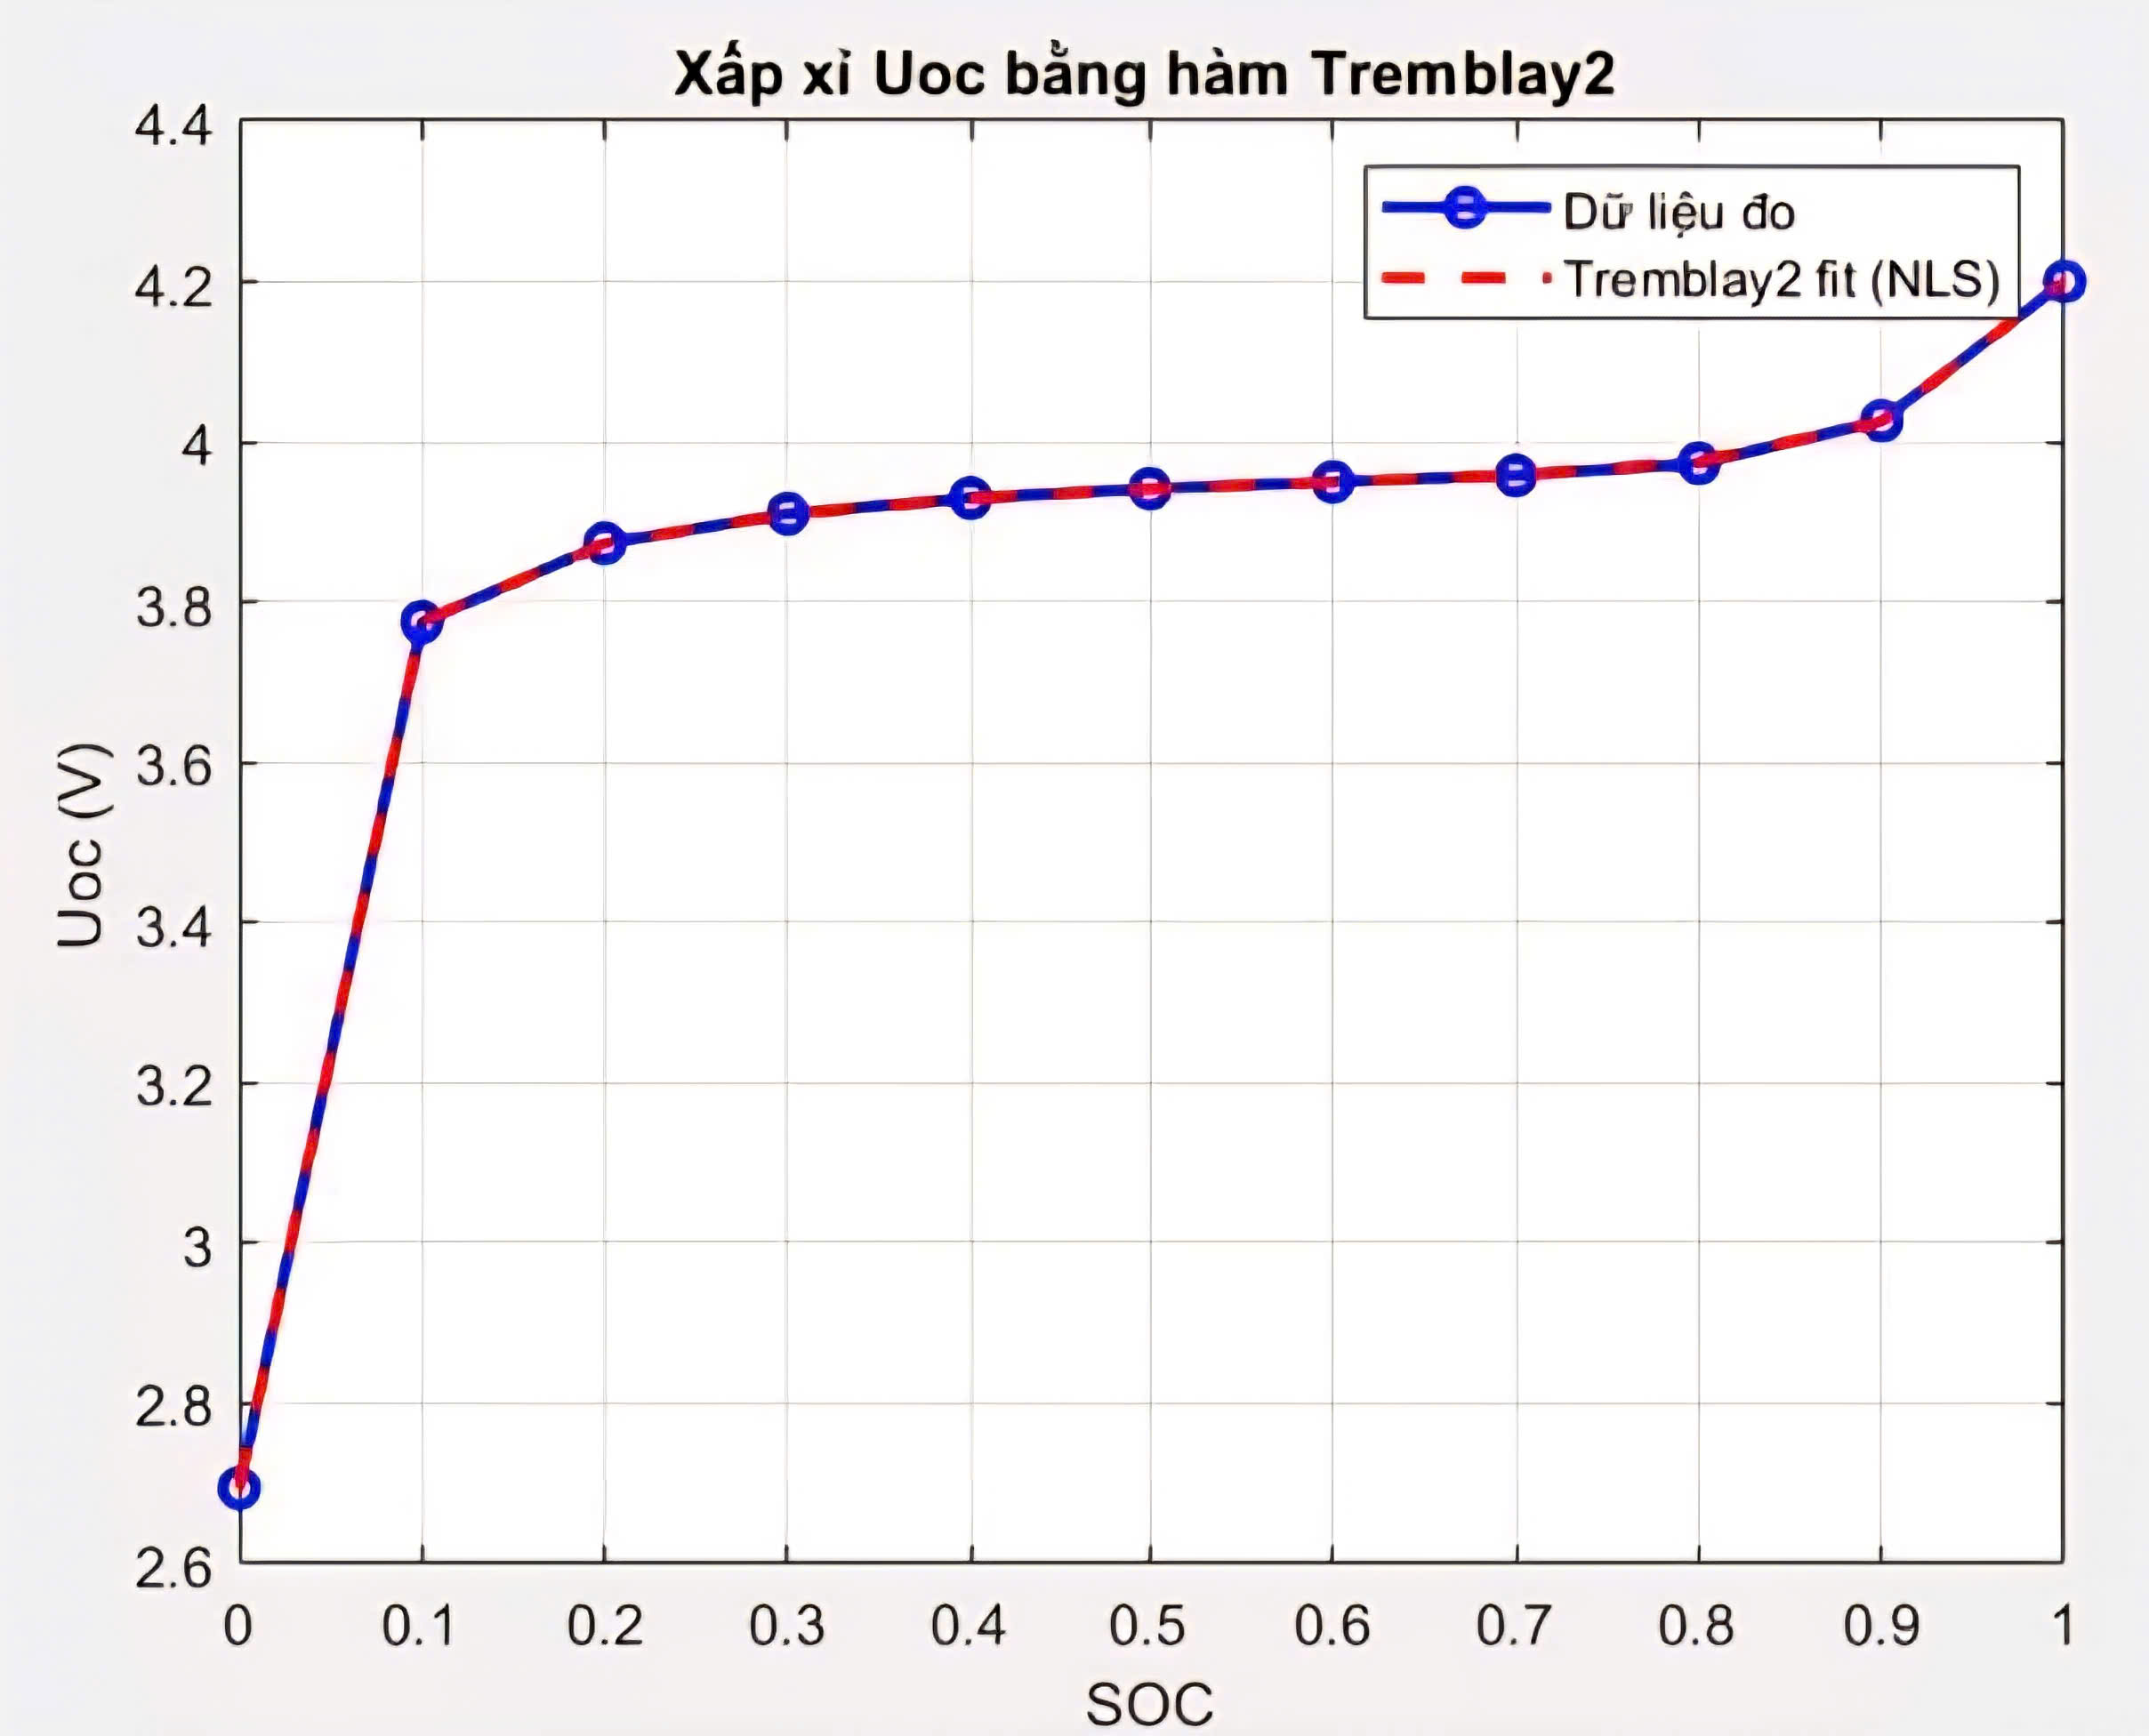
\includegraphics[width=0.8\textwidth]{media/image13.jpg}
    \caption{Đường cong \( U_{oc} \) theo SoC}
    \label{fig:uoc_soc}
\end{figure}



\subsubsection{Biểu diễn \( R \), \( C \) theo SoC}

Hàm đa thức bậc 7 là hàm tối ưu để biểu diễn giá trị nội trở, điện trở và tụ điện phân cực theo SoC:

\begin{equation}
f(SoC) = a_0 + a_1 x + a_2 x^2 + a_3 x^3 + a_4 x^4 + a_5 x^5 + a_6 x^6 + a_7 x^7 
\end{equation}

Ta có các kết quả biểu diễn các giá trị \( R \), \( C \) của mô hình Thevenin và mô hình DP được cho trên bảng dưới đây. Giá trị nội trở \( R_0 \) có kết quả là hằng số và bằng \( 0.05\,\Omega \).   
  
.

\begin{table}[h]
    \centering
    \begin{tabular}{|c|c|c|c|c|c|c|c|c|}
        \hline
        Tham số & \( a_0 \) & \( a_1 \) & \( a_2 \) & \( a_3 \) & \( a_4 \) & \( a_5 \) & \( a_6 \) & \( a_7 \) \\
        \hline
        \( R_p \) & 0.0043 & 0.0117 & -0.2011 & 1.5449 & -5.2581 & 9.0585 & -7.6792 & 2.5635 \\
        \( C_p \) & 3.9333 & -5.1095 & 15.5529 & -73.1474 & 180.9128 & -240.9101 & 163.3745 & -44.2506 \\
        \hline
    \end{tabular}
    \caption{Tham số của đa thức bậc 7 biểu diễn tụ điện và điện trở mô hình Thevenin theo SoC}
    \label{tab:thevenin_poly}
\end{table}

\begin{table}[H]
    \centering
    \resizebox{\textwidth}{!}{%
    \begin{tabular}{|c|c|c|c|c|c|c|c|c|}
        \hline
        Tham số & \( a_0 \) & \( a_1 \) & \( a_2 \) & \( a_3 \) & \( a_4 \) & \( a_5 \) & \( a_6 \) & \( a_7 \) \\
        \hline
        \( R_1 \) & 0.0032 & 0.0275 & -0.3812 & 2.4196 & -7.4570 & 12.0042 & -9.6662 & 3.0886 \\
        \( C_1 \) & 4.5004 & -9.2253 & 58.0669 & -277.4098 & 677.9682 & -887.5461 & 592.4562 & -158.4105 \\
        \( R_2 \) & 0.0012 & -0.0191 & 0.2184 & -1.0772 & 2.7561 & -3.7670 & 2.5989 & -0.7055 \\
        \( C_2 \) & 25.7873 & 253.5 & -3192.3 & 15380.5 & -37793.2 & 49713.4 & -33332.1 & 8947.8 \\
        \hline
    \end{tabular}%
    }
    \caption{Tham số của đa thức bậc 7 biểu diễn tụ điện và điện trở mô hình DP theo SoC}
    \label{tab:dp_poly}
\end{table}

\newpage

    \section*{CHƯƠNG 5. ĐÁNH GIÁ SAI SỐ VÀ SO SÁNH MÔ HÌNH QUA QUÁ TRÌNH SẠC CC-CV}
    \addcontentsline{toc}{section}{\numberline{} CHƯƠNG 5. ĐÁNH GIÁ SAI SỐ VÀ SO SÁNH MÔ HÌNH QUA QUÁ TRÌNH SẠC CC-CV}
    \setcounter{section}{5}
    \setcounter{subsection}{0}
    \setcounter{figure}{0}
    \setcounter{table}{0}
    
    \subsection{Phương pháp sạc ổn dòng, ổn áp (CC-CV)}
    \subsubsection{Cơ sở lý thuyết}
    Phương pháp sạc ổn dòng, ổn áp là phương pháp kết hợp giữa hai phương pháp ổn dòng (CC) và phương pháp ổn áp (CV). Đây là phương pháp sạc pin Lithium-ion phổ biến nhất hiện nay \cite{shen2012}.

    Quá trình sạc bao gồm 2 giai đoạn CC, CV thể hiện như lưu đồ Hình \ref{fig:cccv_flow}. Bắt đầu với giai đoạn CC, pin được sạc bằng dòng cố định ($I_{cc}$) cho đến khi điện áp đạt tới điện áp ngưỡng xác định ($U_{cutoff}$). Sau đó, trong giai đoạn CV, điện áp pin giữ ở mức điện áp ngưỡng, và dòng sạc giảm dần xuống dưới mức dòng cutoff (dòng điện ngưỡng), kết thúc quá trình sạc. Hình 5.2. biểu diễn dạng sóng dòng điện, điện áp pin của phương pháp sạc CC-CV.

    \begin{figure}[H]
        \centering
        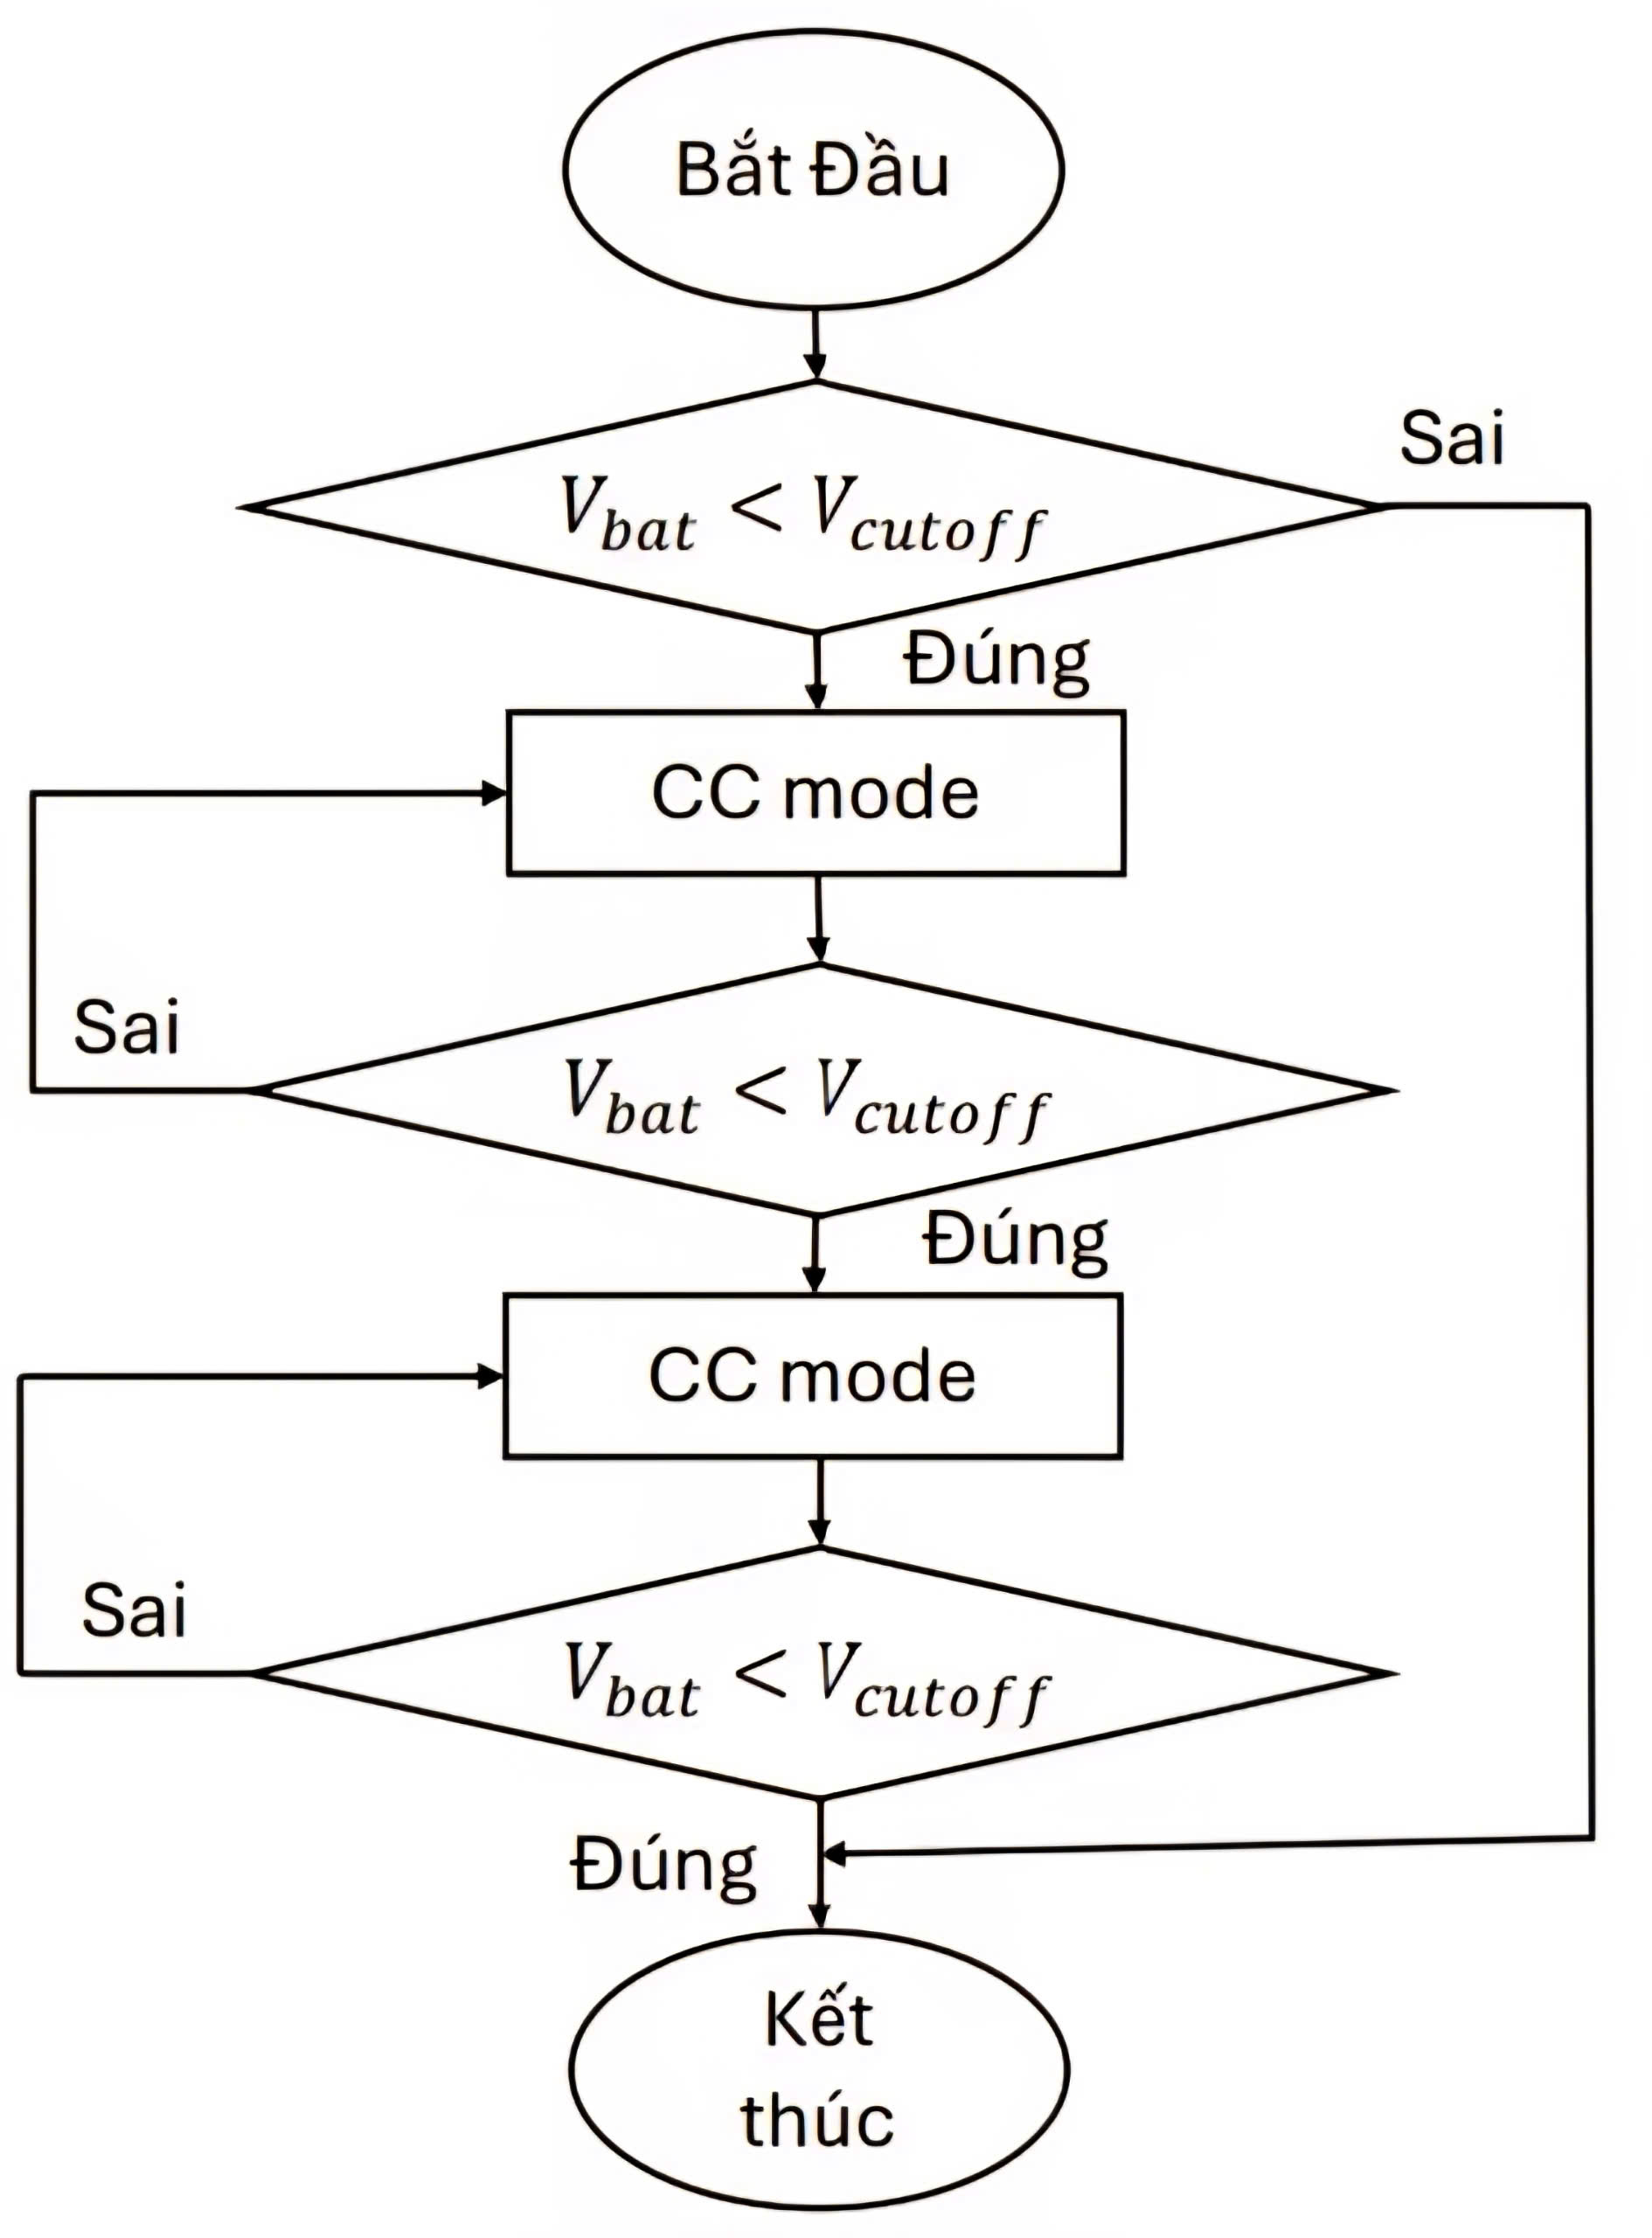
\includegraphics[width=0.6\textwidth]{media/image14.jpg}
        \caption{Lưu đồ thuật toán phương pháp CC-CV}
        \label{fig:cccv_flow}
    \end{figure}

    \begin{figure}[H]
        \centering
        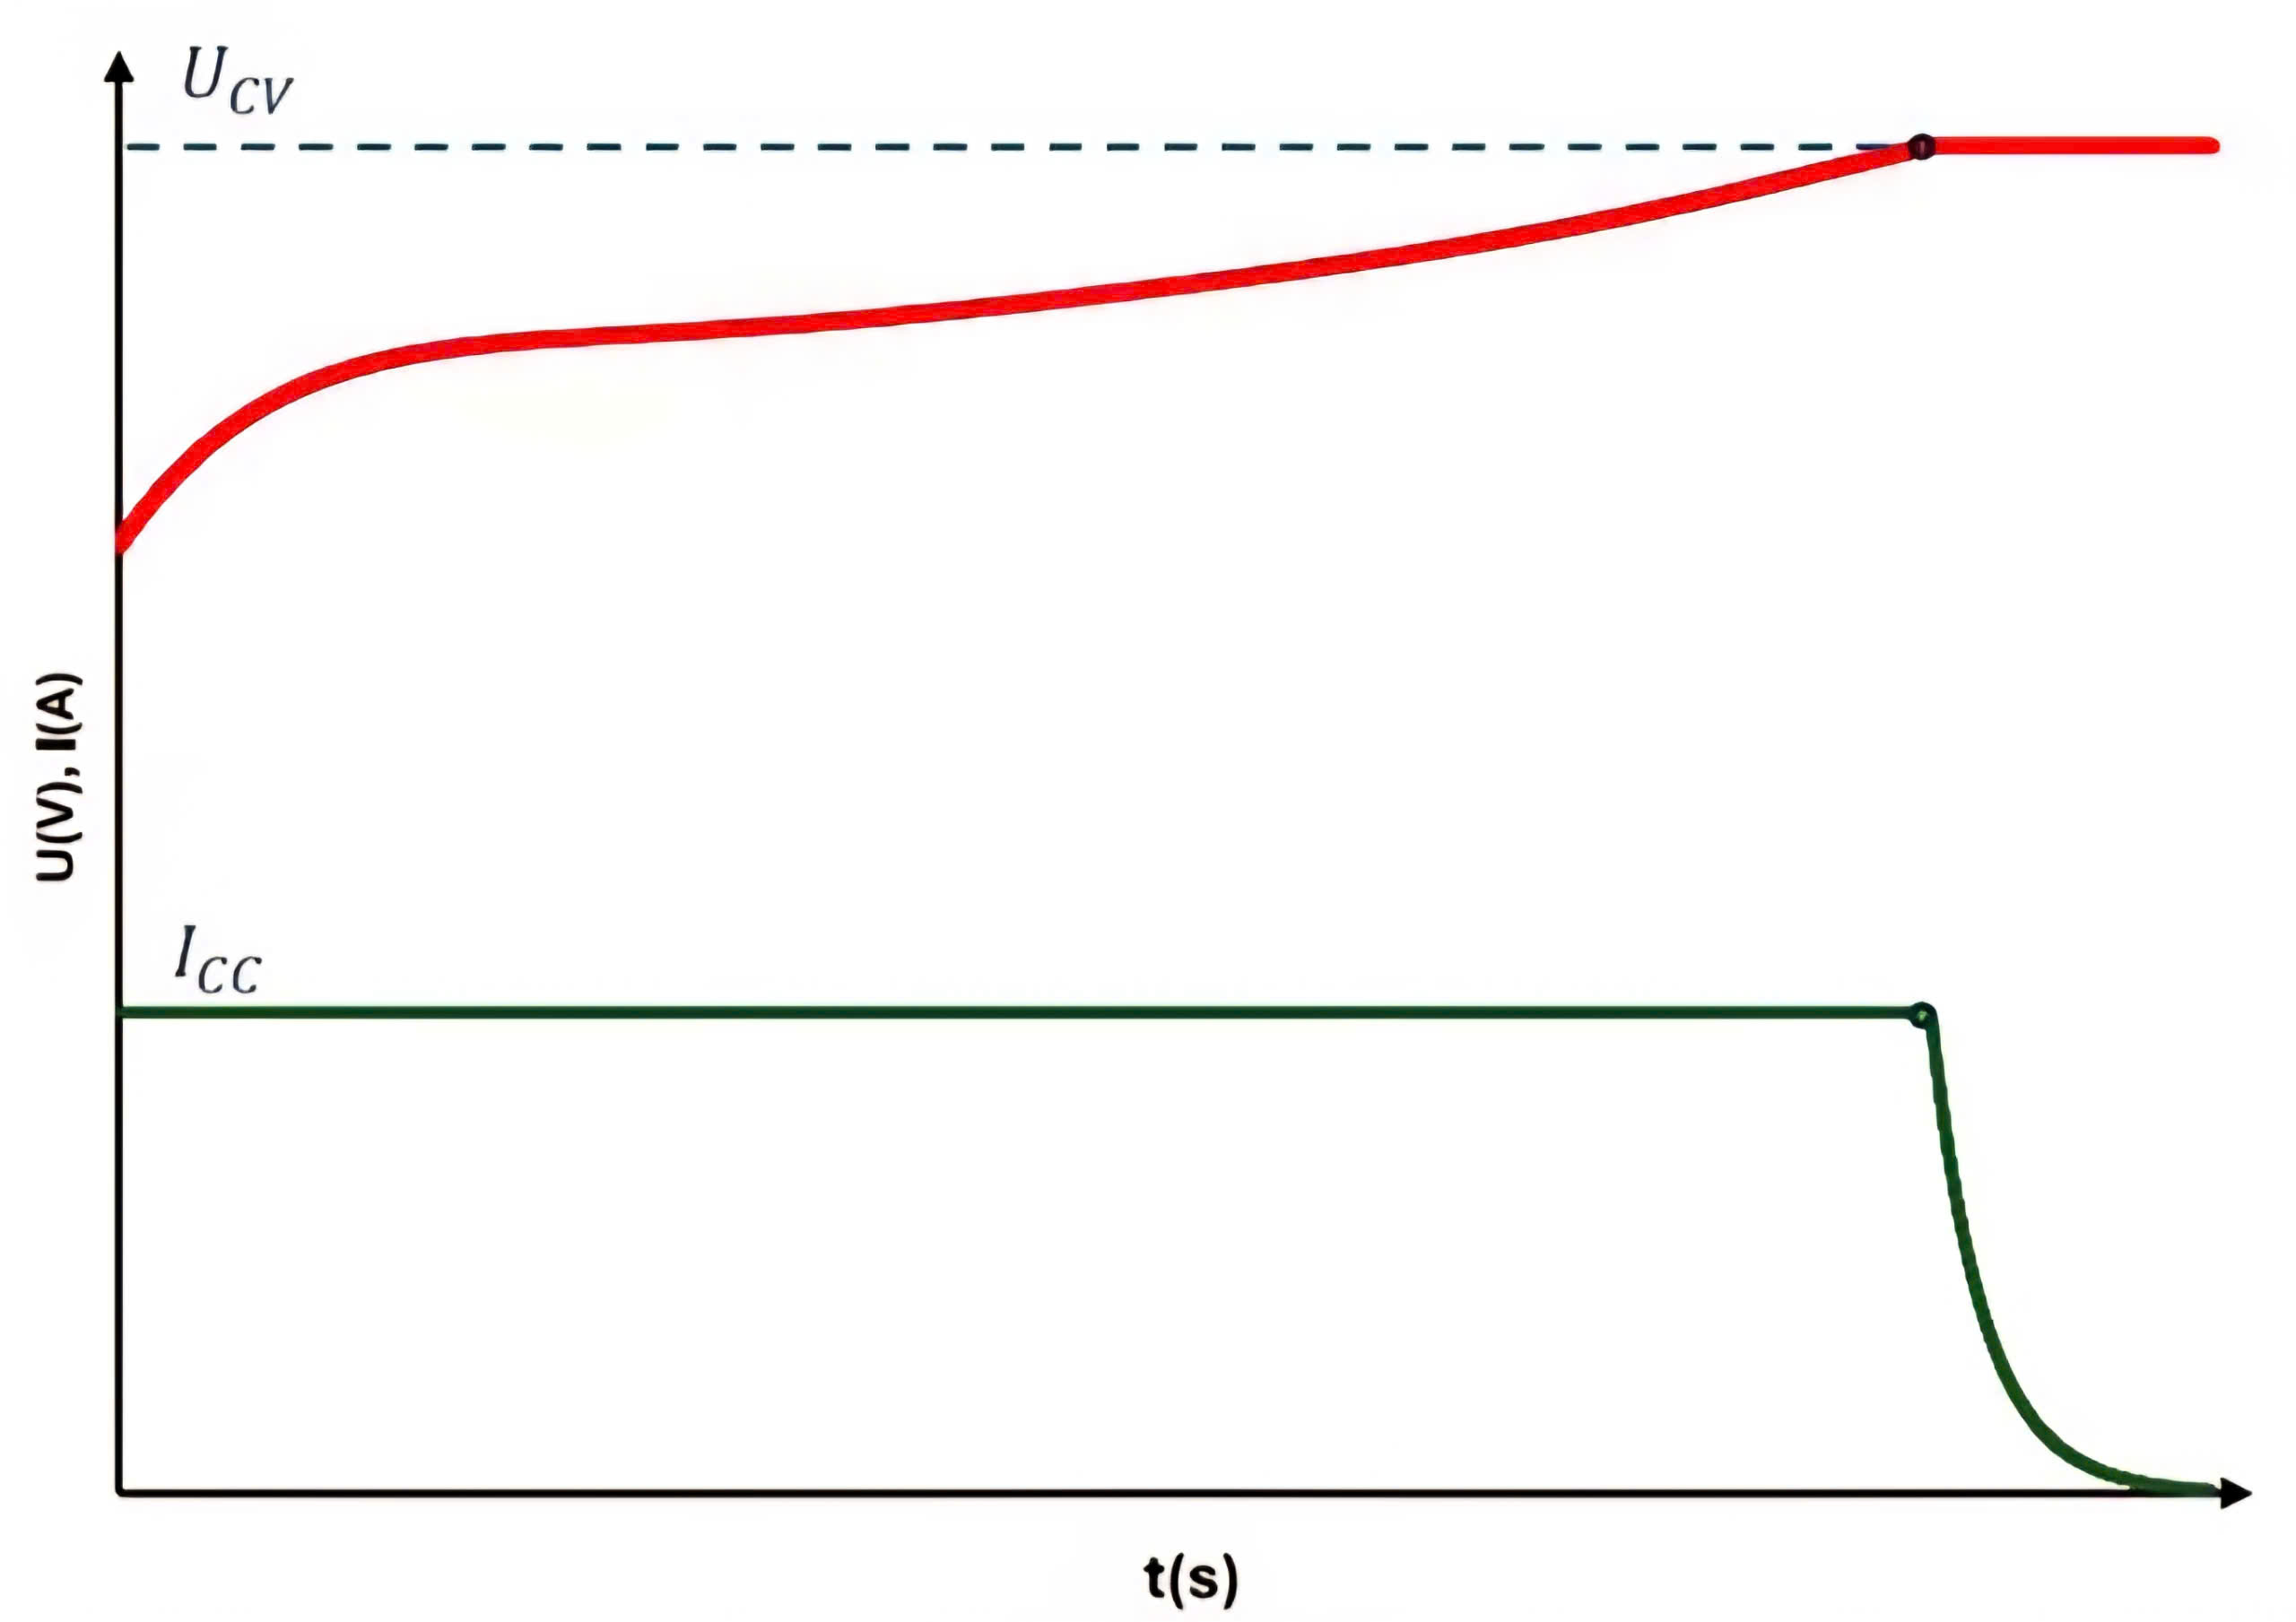
\includegraphics[width=0.8\textwidth]{media/image15.jpg}
        \caption{Đồ thị dòng, áp sạc phương pháp CC-CV}
        \label{fig:cccv_graph}
    \end{figure}

    Phương pháp sạc CC-CV là phương pháp được sinh ra để khắc phục nhược điểm của hai phương pháp CC và CV. Đối với phương pháp sạc CV, do điện áp trên pin thay đổi nhanh chóng từ $OCV_0$ lên điện áp ngưỡng nên dòng điện ban đầu vượt quá giới hạn sạc ảnh hưởng đến tuổi thọ của pin, không những vậy, dòng điện trung bình của phương pháp sạc CV bé, điều này cũng làm thời gian sạc của phương pháp CV lâu hơn. Đối với phương pháp sạc CC, dung lượng pin được sạc giảm xuống do có điện áp rơi trên nội trở của pin lớn. Phương pháp sạc CC-CV ban đầu cho tăng điện áp từ từ với dòng sạc ổn định để giải quyết nhược điểm của phương pháp CV và bù lượng dung lượng còn thiếu của phương pháp sạc CC bằng cách thêm giai đoạn CV vào sau, do trong chế độ CV dòng điện giảm dần nên điện áp rơi trên trở cũng giảm xuống.

    Phương pháp sạc CC-CV dù là phương pháp phổ biến và hiệu quả cho pin Lithium-ion, vẫn tồn tại một số nhược điểm đáng chú ý. Trước hết, thời gian sạc trong giai đoạn CV kéo dài do dòng sạc giảm dần từ mức ngưỡng xuống $I_{cutoff}$, khiến quá trình sạc không đáp ứng được nhu cầu sạc nhanh. Thứ hai, hiệu quả của phương pháp này phụ thuộc lớn vào việc lựa chọn thông số tối ưu như dòng sạc $I_{cc}$ và điện áp ngưỡng $U_{cutoff}$; nếu các thông số này không được tinh chỉnh chính xác, pin có thể bị lão hóa nhanh do nhiệt độ tăng hoặc thời gian sạc bị kéo dài không cần thiết. Cuối cùng, việc kết hợp hai giai đoạn CC và CV làm tăng độ phức tạp của bộ sạc và hệ thống quản lý pin (BMS), dẫn đến chi phí sản xuất cao hơn và yêu cầu phần cứng tiên tiến để đảm bảo chuyển đổi mượt mà giữa các giai đoạn. Những hạn chế này đặt ra thách thức trong việc phát triển các giao thức sạc nhanh và bền vững hơn cho xe điện trong tương lai.

    \subsubsection{Mô phỏng }
    Việc mô phỏng quá trình sạc CC-CV cho từng mô hình mạch điện tương đương của pin được thực hiện bằng phần mềm PSIM. Trong đó pin được sạc với dòng 1.1A, điện áp 4.2V và các thành phần nguồn áp, điện trở, tụ điện phụ thuộc vào SoC được xây dựng bằng các khối logic có trong phần mềm. Các Hình 5.3., Hình 5.4., và hình 5.5.. 
    \begin{figure}[H]
        \centering
        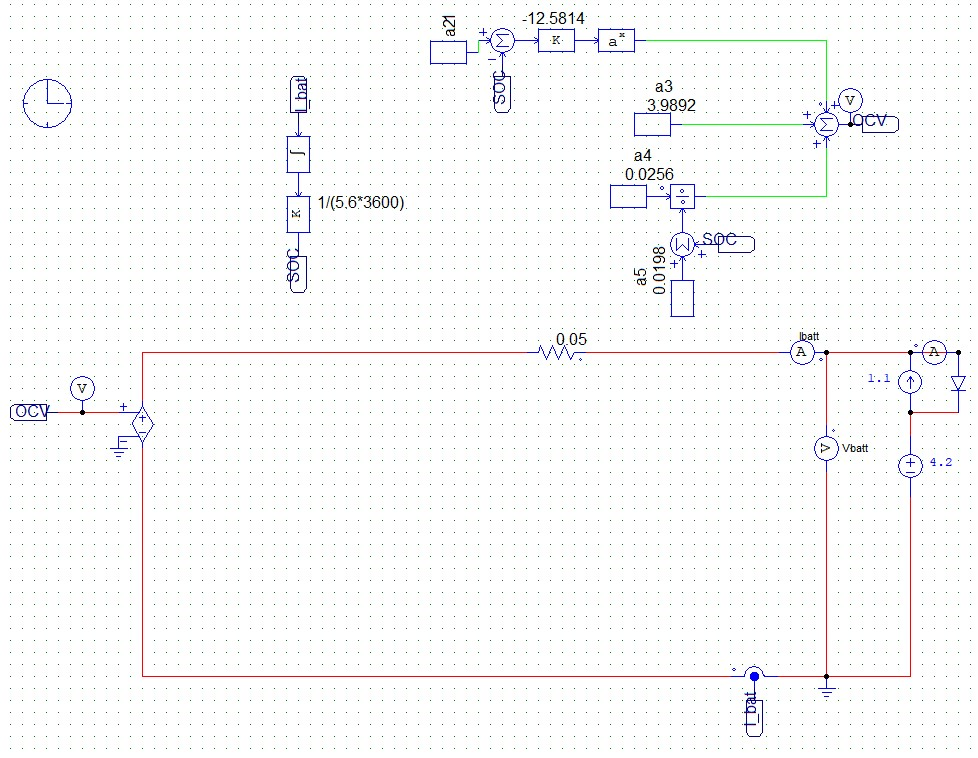
\includegraphics[width=0.5\textwidth]{media/mp-Rint.jpg}
        \caption{Mô phỏng sạc CC-CV cho mô hình Rint}
        \label{fig:cccv_graph}
    \end{figure}
    \begin{figure}[H]
        \centering
        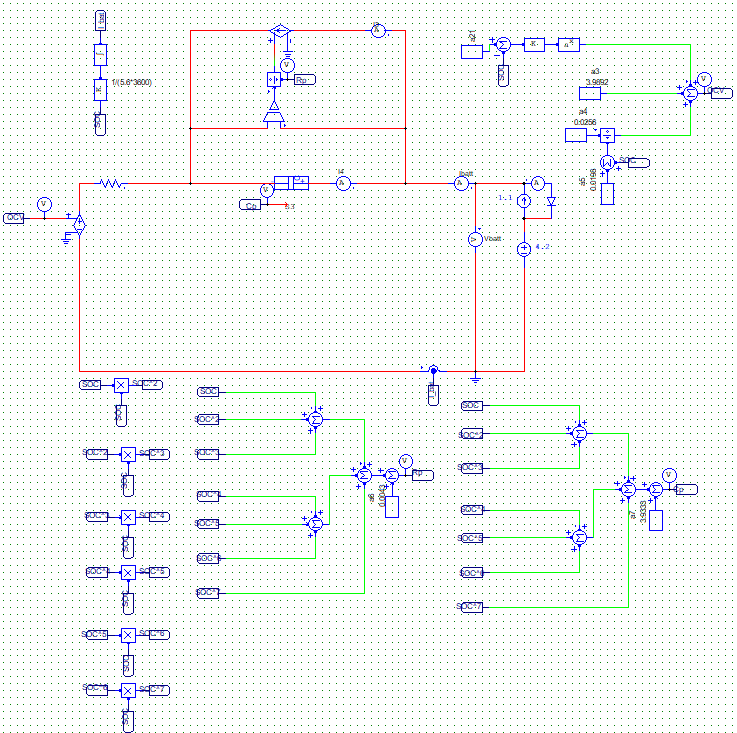
\includegraphics[width=0.8\textwidth]{media/mp-Thevenin.png}
        \caption{Mô phỏng sạc CC-CV cho mô hình Thevenin}
        \label{fig:cccv_graph}
    \end{figure}
    \begin{figure}[H]
        \centering
        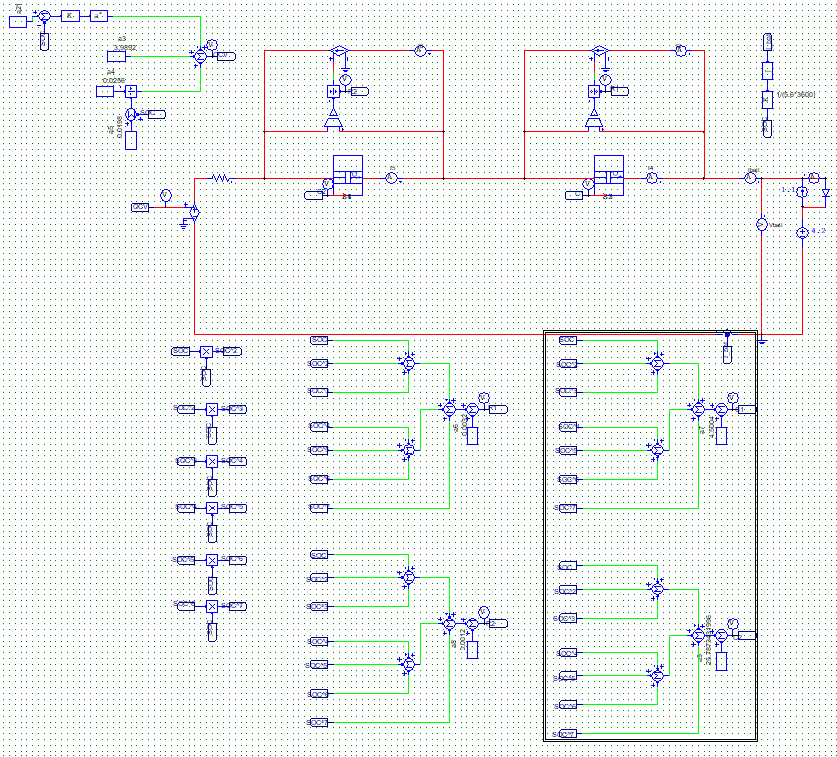
\includegraphics[width=0.8\textwidth]{media/mp-DP.png}
        \caption{Mô phỏng sạc CC-CV cho mô hình DP}
        \label{fig:cccv_graph}
    \end{figure}
    \subsection{Đồ thị đáp ứng điện áp của mô hình và thực nghiệm}
    Tính chính xác của mô hình pin được kiểm chứng bằng cách so sánh đồ thị của đáp ứng điện áp sạc CC-CV giữa mô hình và thực nghiệm. Hình \ref{fig:voltage_compare} cho thấy sự tương đồng về đường cong điện áp sạc của 3 mô hình (đường màu xanh) và thực nghiệm (đường nét đứt màu đỏ). Tuy nhiên, để so sánh chi tiết hơn về tính chính xác của 3 mô hình ta cần phải xét đến các sai số như RMSE, MPE và phương sai.

    \begin{figure}[H]
        \centering
        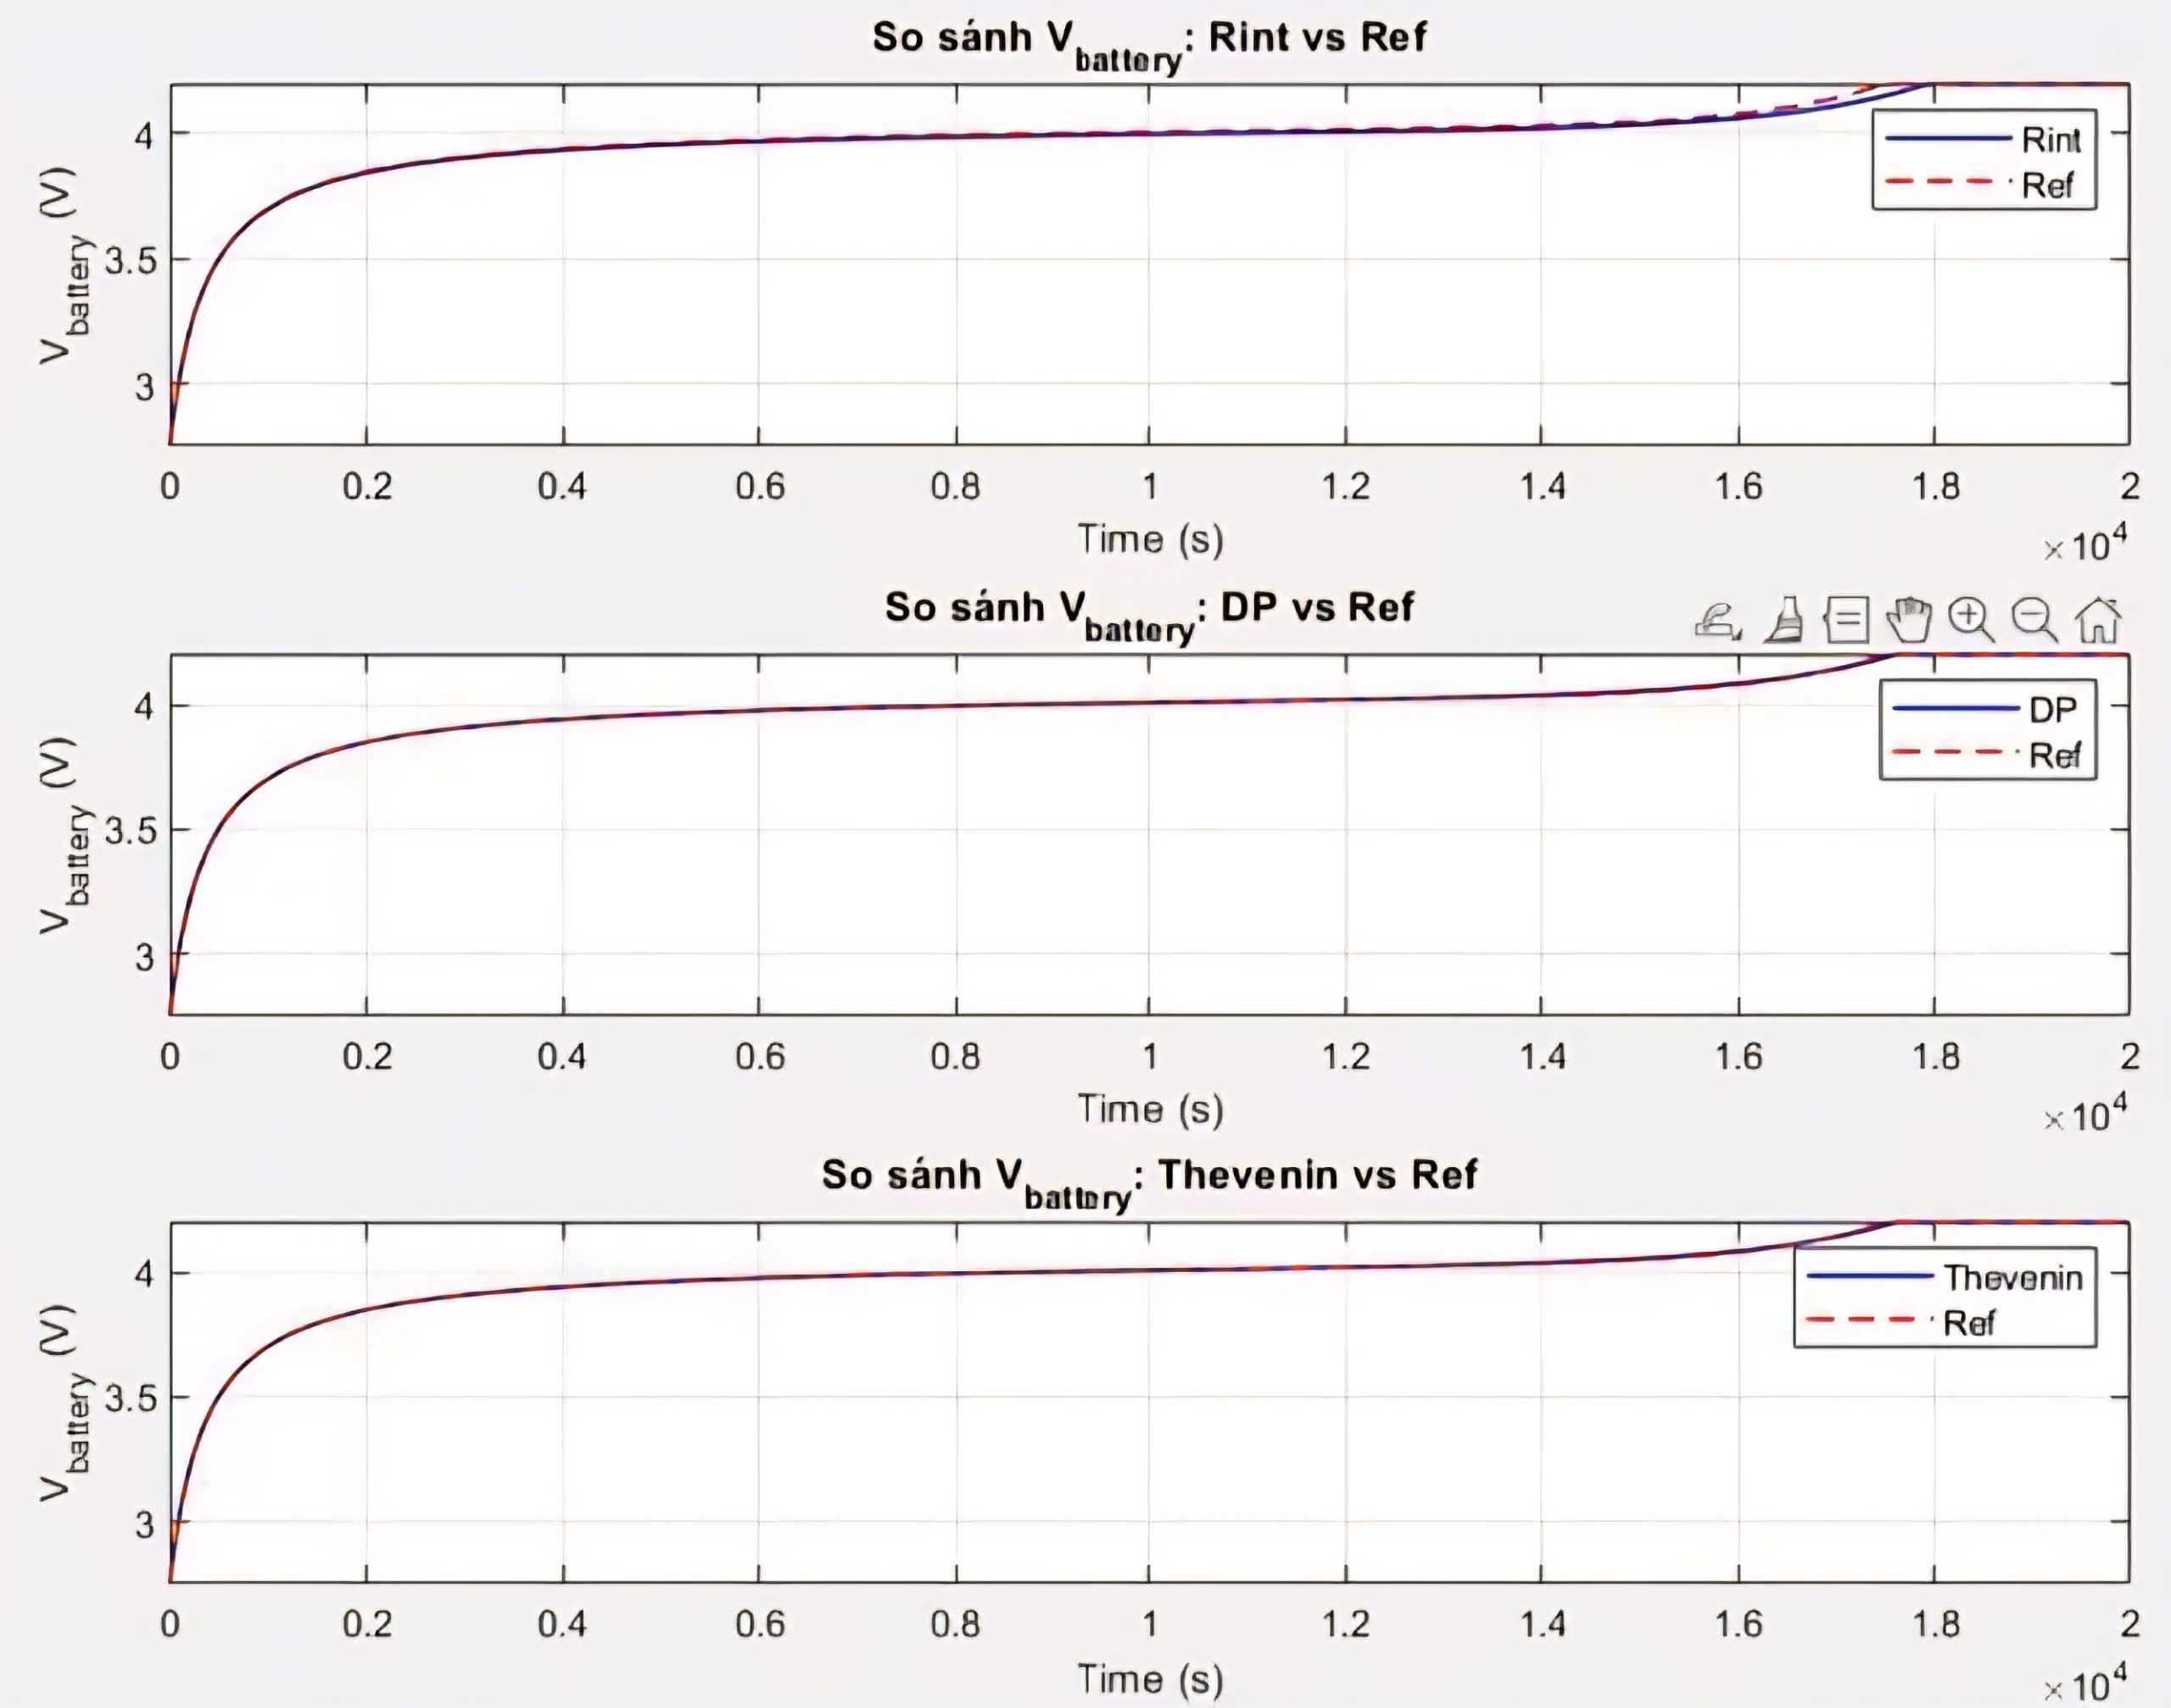
\includegraphics[width=0.8\textwidth]{media/image16.jpg}
        \caption{So sánh đồ thị điện áp sạc các mô hình với thực nghiệm}
        \label{fig:voltage_compare}
    \end{figure}

    \subsection{Sai số đáp ứng điện áp giữa mô hình và thực nghiệm}
    \subsubsection{Root Mean Square Error (RMSE)}
    RMSE phản ánh mức độ sai lệch trung bình của mô hình trên toàn bộ tập dữ liệu \cite{nemes2019}. Công thức tính RMSE được cho như sau:

\begin{equation}
RMSE = \sqrt{\frac{\sum_{i=1}^{N} (v_t - v_t')^2}{N}}
\end{equation}

Trong đó, \( v_t \) và \( v_t' \) lần lượt là điện áp thực nghiệm (V) và điện áp mô hình (V) tại thời điểm \( i \), \( N \) là số lượng điểm dữ liệu. Áp dụng công thức này để tính RMSE của đáp ứng điện áp giữa các mô hình thực nghiệm với \( N = 1000000 \), kết quả được trình bày trong Bảng 4.1.
\newpage
\begin{table}[h]
    \centering
    \begin{tabular}{|c|c|}
        \hline
        Mô hình & RMSE (V) \\
        \hline
        Rint & 0.012114 \\
        Thevenin & 0.002430 \\
        DP & 0.002419 \\
        \hline
    \end{tabular}
    \caption{RMSE của các mô hình}
    \label{tab:rmse}
\end{table}

\subsubsection{Maximum Percentage Error (MPE)}

MPE phản ánh trường hợp sai lệch lớn nhất của mô hình \cite{zhang2010}. Công thức tính MPE được biểu diễn như sau:

\begin{equation}
MPE = \max\left(\left|\frac{v_t - v_t'}{v_t}\right|\right) \times 100\%
\end{equation}

Trong đó, \( v_t \) và \( v_t' \) lần lượt là điện áp thực nghiệm (V) và điện áp mô hình (V) tại thời điểm \( i \). Áp dụng công thức này để tính MPE của đáp ứng điện áp giữa các mô hình thực nghiệm với 1000000 điểm dữ liệu, kết quả được trình bày trong Bảng 4.2.

\begin{table}[h]
    \centering
    \begin{tabular}{|c|c|}
        \hline
        Mô hình & MPE (\%) \\
        \hline
        Rint & 1.170329 \\
        Thevenin & 0.344401 \\
        DP & 0.342556 \\
        \hline
    \end{tabular}
    \caption{MPE của các mô hình}
    \label{tab:mpe}
\end{table}


\subsubsection{Phương sai (Variance)}

Phương sai đo mức độ dao động của sai số quanh giá trị trung bình \cite{he2011}. Công thức tính phương sai được cho như sau:

\begin{equation}
\text{Variance} = \frac{1}{N} \sum_{i=1}^{N} (v_i - \bar{v})^2
\end{equation}

Nếu phương sai cao, sai số bị phân tán, mô hình có thể dự đoán tốt ở một số thời điểm nhưng lại lệch nhiều ở những thời điểm khác, dẫn đến mô hình không ổn định và ảnh hưởng đến độ chính xác. Kết quả phương sai của các mô hình được trình bày trong Bảng 4.3.

\begin{table}[H]
    \centering
    \begin{tabular}{|c|c|}
        \hline
        \textbf{Model} & \textbf{Variance (\(V^2\))} \\
        \hline
        Rint     & \(5.78 \times 10^{-5}\) \\
        Thevenin & \(5.81 \times 10^{-6}\) \\
        DP       & \(5.75 \times 10^{-6}\) \\
        \hline
    \end{tabular}
    \caption{Phương sai của các mô hình}
    \label{tab:variance}
\end{table}


\subsection{Đánh giá và nhận xét}

Bảng 4.4 tổng hợp các giá trị sai số đáp ứng điện áp của các mô hình so với thực nghiệm. Kết quả cho thấy, như đã trình bày ở mục 1.4.3, mô hình DP đạt độ chính xác cao nhất, tiếp theo là mô hình Thevenin, và thấp nhất là mô hình Rint. Tuy nhiên, mô hình DP có độ phức tạp cao nhất do chứa hai nhánh RC song song, dẫn đến số lượng phương trình toán học đáng kể, làm tăng tài nguyên tính toán và thời gian xác định mô hình. Trong khi đó, mô hình Thevenin cân bằng tốt giữa độ chính xác và độ phức tạp, trở thành lựa chọn tối ưu.

\begin{table}[h]
    \centering
    \begin{tabular}{|c|c|c|c|}
        \hline
        Mô hình & RMSE (V)& MPE (\%) & Phương sai (c)\\
        \hline
        Rint & 0.045 & 2.50 & 0.0020 \\
        Thevenin & 0.030 & 1.80 & 0.0009 \\
        DP & 0.015 & 0.90 & 0.0004 \\
        \hline
    \end{tabular}
    \caption{Tổng hợp sai số các mô hình}
    \label{tab:summary}
\end{table}


    \section*{KẾT LUẬN}
    \phantomsection\addcontentsline{toc}{section}{\numberline{} KẾT LUẬN}
    Đồ án đã so sánh các mô hình Rint, Thevenin, và DP, trong đó Thevenin cân bằng tốt giữa độ chính xác và độ phức tạp. Các mô hình này được đánh giá dựa trên thí nghiệm HPPC và mô phỏng sạc CCCV, với các sai số RMSE, MPE và phương sai được sử dụng để so sánh độ chính xác. Kết quả cho thấy mô hình DP có độ chính xác cao nhất nhưng phức tạp, trong khi mô hình Rint đơn giản nhưng kém chính xác. Mô hình Thevenin là lựa chọn tối ưu cho các ứng dụng thực tế đòi hỏi cân bằng giữa hiệu suất và chi phí tính toán như xe điện.

    % TÀI LIỆU THAM KHẢO
    \phantomsection\addcontentsline{toc}{section}{\numberline{} TÀI LIỆU THAM KHẢO}
    \bibliographystyle{ieeetr}
    \bibliography{citation}
    \newpage

\end{document}
```